% QUANDO SCRIVI LA TESI RICORDA DI CAMBIARE IL COMPILATORE DELLA BIBLIOGRAFIA IN BIBER (PERCHE' IL PROGETTO DI INTERDISCIPLINARY PROJECT USA BIBTEX). SE TI DIMENTICHI COME CAMBIARLO E' IN OPZIONI > CONFIGURA TEX STUDIO >  COMPILA >  STRUMENTO PREDEFINITO PER LA BIBLIOGRAFIA O QUALCOSA DEL GENERE

\documentclass[a4paper, 12pt]{report}
\usepackage{template}
\usepackage{fancyvrb}
\usepackage{hyperref}
\usepackage{eso-pic}
\usepackage{graphicx}
\usepackage{amsmath}
\usepackage{booktabs}
\usepackage{array}
\usepackage{transparent} % per trasparenza
\DefineVerbatimEnvironment{MyVerbatim}{Verbatim}{baselinestretch=0.8}
\usepackage[backend=biber, style=apa,sorting=nyt, maxnames=2,minnames=1]{biblatex}
\DefineBibliographyStrings{english}{%
	andothers = {\mkbibemph{et\addabbrvspace al\adddot}}}
\addbibresource{Tesi2.bib}
\defbibheading{bibliography}{}
\usepackage[table]{xcolor}
\usepackage{tabularx}
\usepackage{listings}
\lstset{
	basicstyle=\ttfamily\small, % o \footnotesize, \scriptsize
	breaklines=true,
	aboveskip=2pt,
	belowskip=0pt
}

\begin{document}
\sloppy
\mytitlepage{BIOINFORMATICS FOR COMPUTATIONAL GENOMICS}{Genotyping By Sequencing (GBS) for population genetics and phylogenetic studies of non-model plants: the case of \textit{Campanula thyrsoides}, and others.}{Chiara Paleni, PhD}{Professor Carla Lambertini}{Flavia Leotta}{45866A}{2024/2025} 

% \clearpage
\newcommand\BackgroundPic{%
	\put(-0.13\paperwidth,-0.19\paperheight){%
		\parbox[b][\paperheight]{\paperwidth}{%
			\vfill
			\centering
			\transparent{0.20} % livello di trasparenza da 0 (invisibile) a 1 (opaco)
			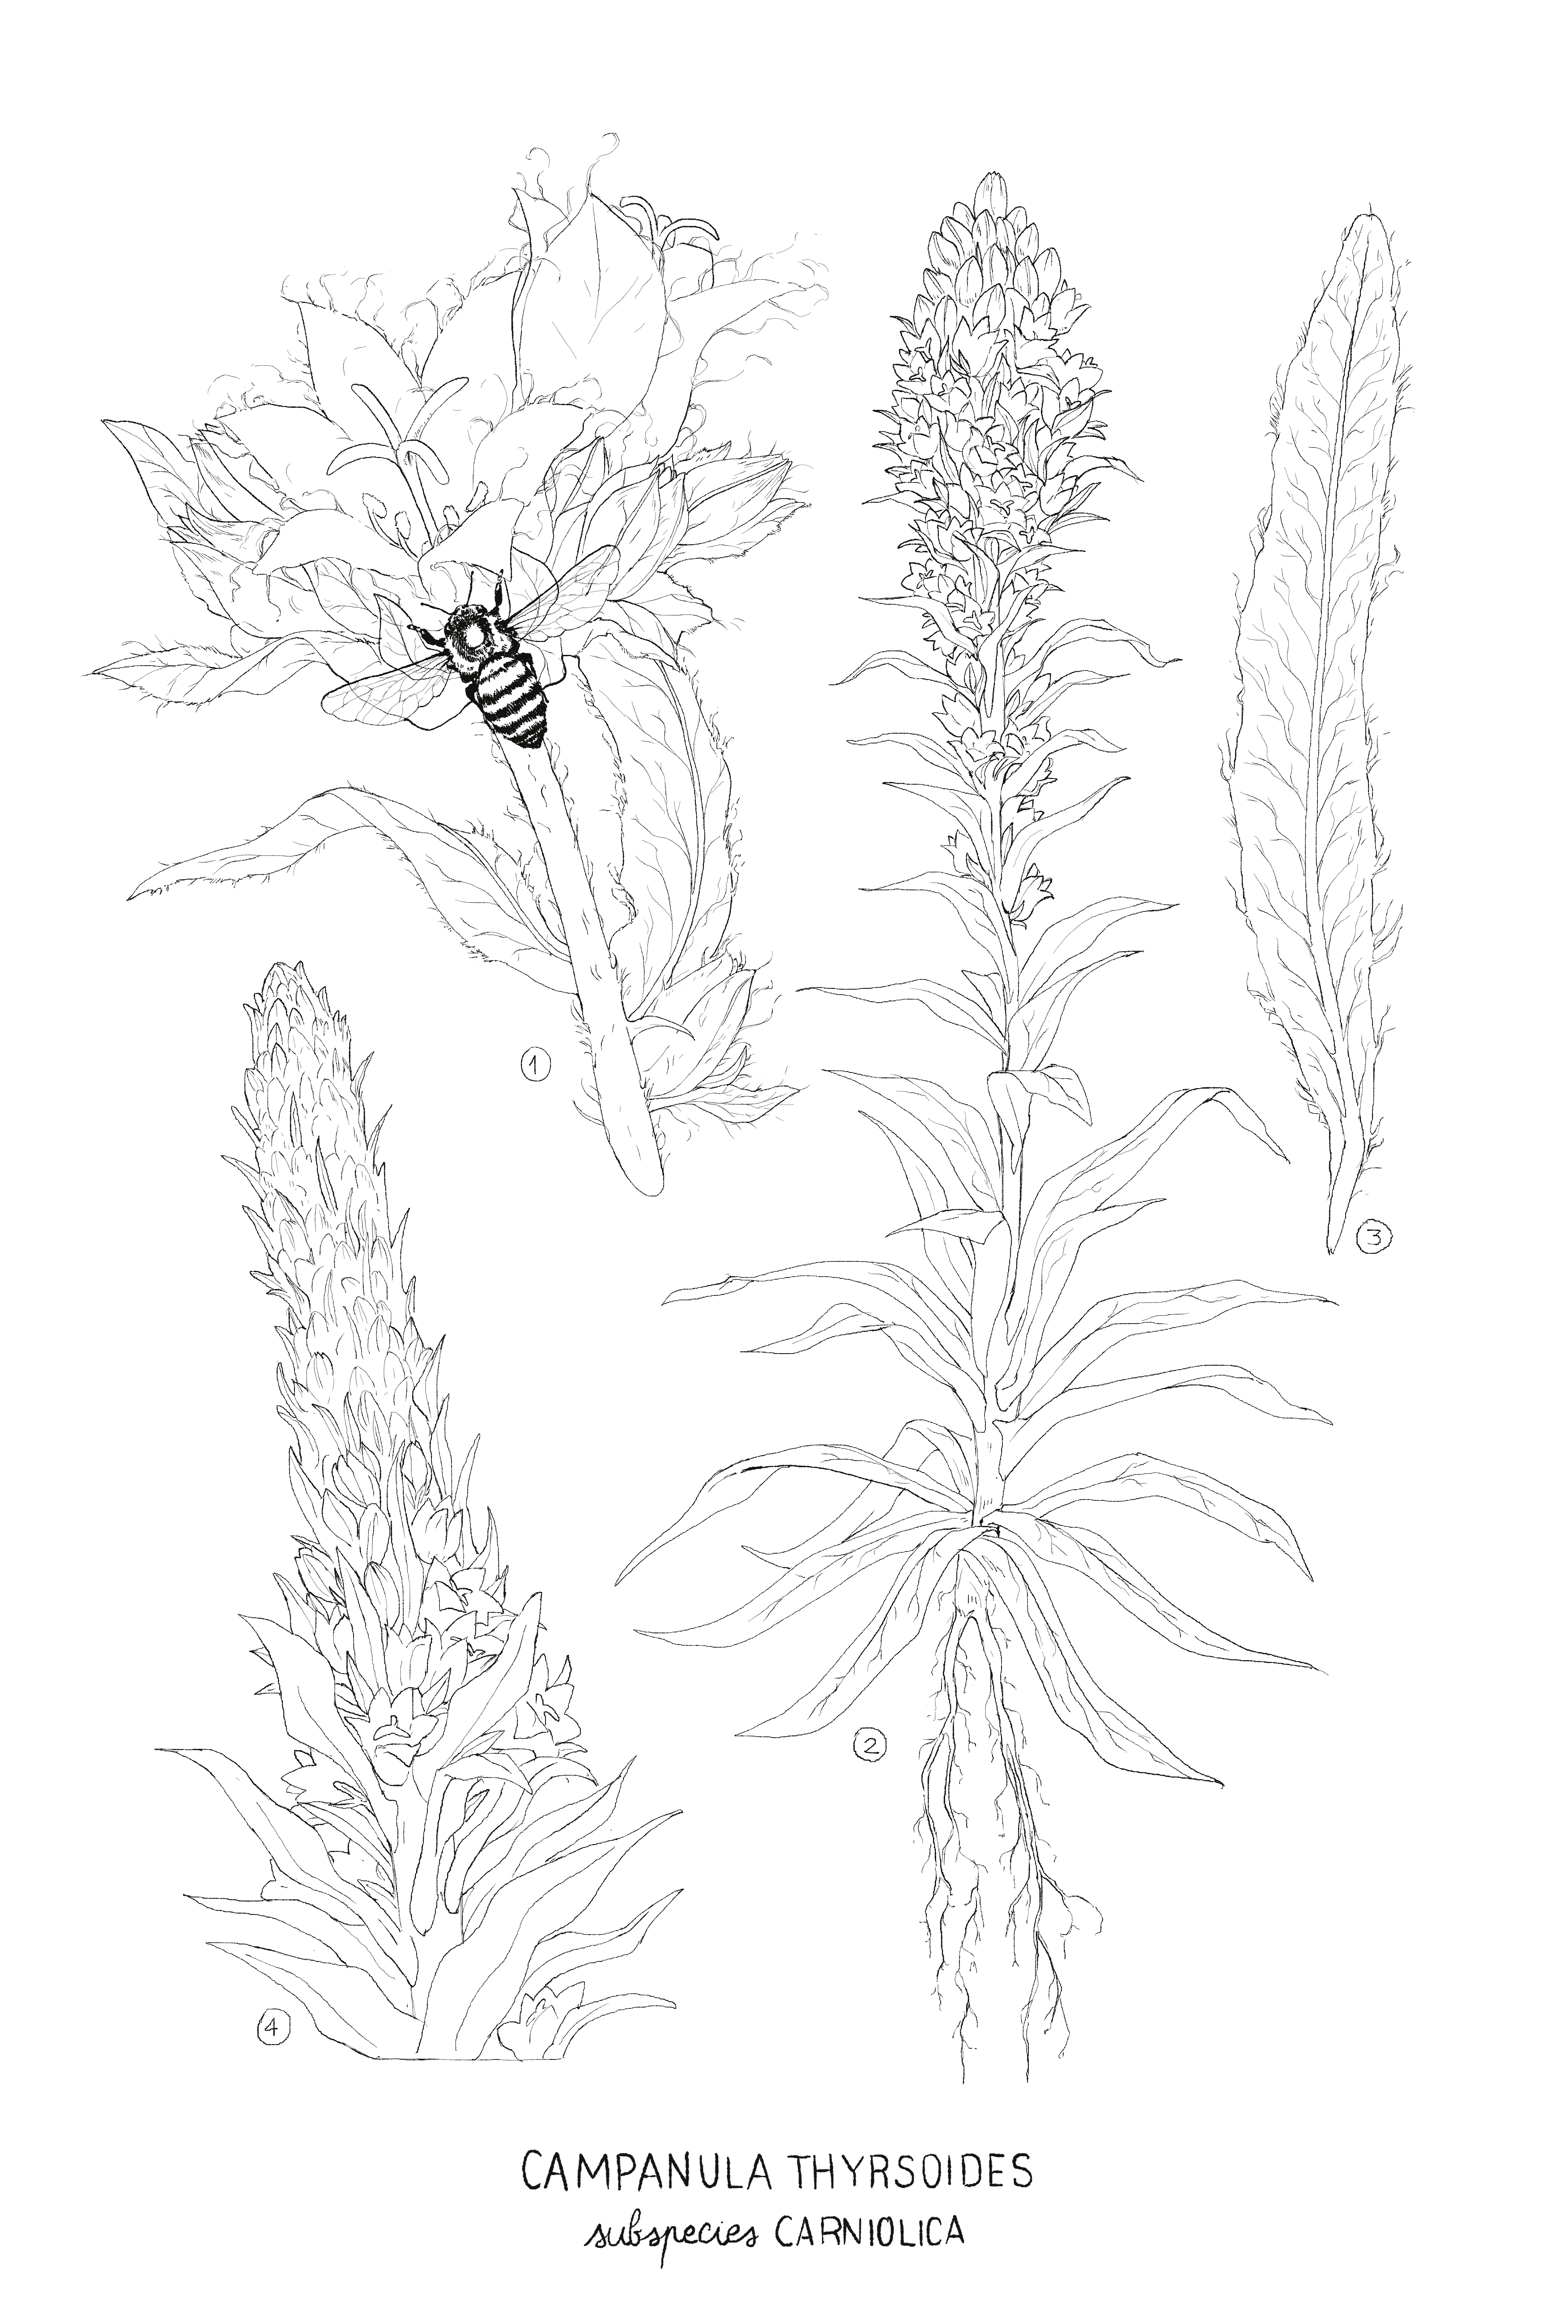
\includegraphics[width=1.3\paperwidth,height=1.3\paperheight,keepaspectratio]{Campanula_thyrsoides_botanic_illustration_bw.png}%
			\vfill
}}}

\AddToShipoutPicture*{\BackgroundPic}
\AddToShipoutPicture*{%
	\put(0.68\paperwidth,0.75\paperheight){%
		\parbox{0.25\paperwidth}{% larghezza del box di testo
			\raggedleft % allinea a destra dentro al box
			\textit{\small
				"May you keep going forward."
			}
		}%
	}%
}
\ClearShipoutPicture

\phantom{}
\pagestyle{empty}
\clearpage


% Abstract
\pagenumbering{roman} % Roman page numbering
\chapter*{Abstract}
This thesis aim is to showcase the use of Genotyping by Sequencing (a Rad-Seq method) for conservation-focused genomic analyses of non-model plants, through three different projects. The first one was a populations genetics study on endemic alpine flower \textit{Campanula thyrsoides} subspecies \textit{carniolica}, carried over 153 individuals spanning 9 populations of interest and 2 outgroup populations (subspecies \textit{thyrsoides}). For this goal SNPs were called using \texttt{Stacks}: \texttt{denovo\_map.pl} pipeline, which provided a matrix of 3896 polymorphic, non rare ($MAF > 0.005$) SNPs. The results showed a good genetic flow between populations with no inbreeding (all $F_{IS} < 0$) while retaining good separation between all populations (pairwise $F_{ST} > 0.10$, $p-value < 10e-16$), with the exception of 3 populations of the same geographical area (Veneto and Friuli-Venezia-Giulia in Italy, with pairwise $F_{ST} \leq 0.10$, $p-value < 10e-16$). PCA and Maximum-Likelihood tree also showed that it was possible to further distinguish samples in Italian, Slovenian and Austrian groups, highlighting a longitude gradient in their genetic information. Furthermore, a population collected in the Italian region of Lombardia, historically habitat of only the subspecies \textit{thyrsoides}, actually clustered with subsp. \textit{carniolica}, showing an increase in this subspecies' habitat. The second project was a phylogenetic study of landraces of \textit{Solanum tuberosum} (modern potato), performed using both GBS data from 12 putative Italian old landraces and 2 commercial cultivars of \textit{S. tuberosum} and WGS data from 4 wild and 4 cultivated Andean species. Using SolTub\_3.0 reference genome and classic tools for genome-based variant calling, we built PCA plots and maximum likelihood trees over 14945 polymorphic SNPs: the results show that while some of the putative Italian lines are indeed alike modern commercial cultivars (Desiree and Kennebec), others are probably the results of different, older evolutionary events. The samples provided by farms in Bossico (BG) and the variety Starleggia bianca from Campodolcino (SO) can be placed, temporally speaking, between wild species (i.e. \textit{S. brevicaule} and \textit{S. chacoense}) and the old, but still cultivated Andean species (i.e. \textit{S. stenotomum} and \textit{S. tuberosum} subsp. \textit{andigenum}). Shilpario, from the Botanical Garden of Bergamo (BG), seems to be born from an older divergence from \textit{S. tuberosum} than the modern cultivars; all the other Italian samples are, instead, close to commercial varieties. Red peel landraces are genetically very close to Desiree, Comasca and the varieties of Quarantina Genoves are more similar to the white-peel modern Kennebec and variety Bianca (SO) can, instead, be seen as an hybrid between the two commercial varieties. The third, and last, project, aims to use double digest RADseq data to explore populations structure of urban and natural populations of orchads \textit{Anacamptis pyramidalis} and \textit{Anacamptis berica}. Using a matrix of 13791 polymorphic, non rare SNPs, we explored the structure of  19 natural (61 samples) and 5 urban populations (29 samples), divided in two species (4 populations of \textit{A. berica} and 20 of \textit{A. pyramidalis}). There is no differentiation neither between populations nor between urban or natural varieties: the pipeline is able, though, to capture the distance between the two species.

% Table of Contents
\clearpage
\chapter*{Table of contents}
\tableofcontents
\clearpage

% Reapply the page style to ensure consistency
\pagestyle{fancy}
\pagenumbering{arabic} % Switch to Arabic numerals for the main content

% Introduction
\chapter{Introduction}
\section{Biodiversity conservation}
Many plant species populations are declining due to human activity  (\cite{suppleConservationBiodiversityGenomics2018}; \cite{yinPlantConservationAge2024}): overexplotation and habitat destruction threat diversity \parencite{penceDefiningExceptionalSpecies2022} and lead to fragmentation and isolation of populations, susceptible to decline and ultimately extinction (\cite{aguilarGeneticConsequencesHabitat2008}; \cite{iucn/sscGuidelinesUseEx2014}). Diversity can be assessed on different levels depending on species \parencite{habelBurdenGeneticDiversity2012}, but it is possible to recognize three main types: between species, between populations of the same species and between individuals of different populations \parencite{salgotraGeneticDiversityConservation2023}. All of these types of diversity concur together to form biodiversity of an ecosystem. The main causes of genetic diversity changes are mutation, gene flow and genetic drift \parencite{salgotraGeneticDiversityConservation2023}, but it can also be influenced by human intervention: while wild species suffer from habitat fragmentation (\cite{aguilarGeneticConsequencesHabitat2008}; \cite{habelBurdenGeneticDiversity2012}), crop plants are instead artificially selected for high yielding, which lowers their genetic diversity \parencite{salgotraGeneticDiversityConservation2023}. Under environmental changes, different populations might survive depending on the presence of favorable genetic characteristics; if, however, populations possess little or no genetic diversity, they could become more susceptible to this action, their individuals might experience loss of fitness \parencite{habelBurdenGeneticDiversity2012} and, in the worst cases, whole populations might fail to adapt \parencite{suppleConservationBiodiversityGenomics2018} and could not survive the stressful event \parencite{salgotraGeneticDiversityConservation2023}. Normally, biotic and abiotic stress aids natural selection, a process that drives evolution and speciation, but when this is caused by human activity, it becomes essential to limit its influence and apply strategies of both \textit{in situ} preservation and \textit{ex situ} conservation \parencite{iucn/sscGuidelinesUseEx2014}. The first term refers to the conservation of genetic resources in a natural habitat \parencite{vijayanGermplasmConservationMulberry2011}, while \textit{ex situ} conservation is carried on in research institutes, botanical gardens or, in general, away from the original habitat of the species, where individuals are maintained under artificial conditions \parencite{iucn/sscGuidelinesUseEx2014}. \textit{Ex-situ} conservation techniques often have a final \textit{in-situ} output \parencite{volisQuasiSituBridge2010}. For example, seed banking (drying at c.15\% relative humidity and then storing at 20°C), arguably the most used, low-cost and effective long-term \textit{ex situ} method  (\cite{volisQuasiSituBridge2010}; \cite{penceDefiningExceptionalSpecies2022}, \cite{salgotraGeneticDiversityConservation2023}) is often used to build collections of seeds as material for \textit{in-situ} recovery actions \parencite{volisQuasiSituBridge2010}. Seed banking, though, it is not feasible for a lot of species, for example those which seeds cannot survive freezing \parencite{penceDefiningExceptionalSpecies2022} or with a long germination time \parencite{volisQuasiSituBridge2010}. To bypass these limitations living horticulturally maintained collections can be used, which are able to maintain a viable population as a source of individuals for population restoration (\cite{volisQuasiSituBridge2010}; \cite{iucn/sscGuidelinesUseEx2014}; \cite{penceDefiningExceptionalSpecies2022}) but they are especially sensitive to genetic
erosion, artificial selection and infestation by pathogens \parencite{volisQuasiSituBridge2010}. \textit{In situ} conservation is the best way to conserve the entire genetic diversity of a plant species \parencite{whitlockConsequencesInsituStrategies2016}, thanks to random mating and recombination which are prone to select advantageous mutations: for example, open pollination, which wouldn't be possible in \textit{ex-situ} methods, allows for free exchange of different genotypes \parencite{salgotraGeneticDiversityConservation2023}. It offers healthy competition among members of the population and ensures a dynamic habitat which favors evolution \parencite{vijayanGermplasmConservationMulberry2011}, with no artificial selection (\cite{iucn/sscGuidelinesUseEx2014}; \cite{salgotraGeneticDiversityConservation2023}). The importance of \textit{in situ} preservation is stated by the IUCN itself, which stresses the need for a proper maintenance of diversity in the wild \parencite{whitlockConsequencesInsituStrategies2016} and suggests \textit{ex situ} conservation as part of a broader strategy and as a support for \textit{in situ} conservation \parencite{iucn/sscGuidelinesUseEx2014}. When \textit{in situ} preservation is impracticable due to invasive species and habitat degradation \parencite{hobanOptimalSamplingSeeds2014} a complementary \textit{ex-situ} approach \parencite{salgotraGeneticDiversityConservation2023} or proper management in parks and protected areas can help in overcoming these problems. Differently from \textit{ex situ} \parencite{iucn/sscGuidelinesUseEx2014}, though, IUCN does not provide specific guidance for \textit{in-situ} preservation, especially for wild species with low potential utility value (e.g. species not related to crop plants; \cite{whitlockConsequencesInsituStrategies2016}). Nevertheless, this kind of conservation requires areas to be protected from human activity \parencite{suppleConservationBiodiversityGenomics2018} and necessitates research and monitoring activities which are the focus of many research institutes in the world. Since genetic diversity is essential for survival of both crop plants \parencite{reddyReviewPotatoSolanum2018} and wild ones, its assessment should be taken as the first step towards conservation programs.

\section{The genomic era of conservation}
When traditional \textit{ex-situ} methods for genetic resources monitoring and conservation are not feasible, plant biotechnology provides tools to mitigate negative effects, especially on crop and model plants \parencite{yinPlantConservationAge2024} but also on rare, ornamental and medicinal species \parencite{salgotraGeneticDiversityConservation2023}. These applications include, but are not limited to genome editing \parencite{suppleConservationBiodiversityGenomics2018} and recombinant technologies \parencite{salgotraGeneticDiversityConservation2023}, proven advantageous in comparison to conventional mutagenesis methods for traits improvement, but also center of controversies due to their generation of transgenic plants, recognized as GMOs \parencite{yinPlantConservationAge2024}. Even genome editing approaches, though, need prior consultation from an interdisciplinary team, comprehending of biotechnologists, ecologists and bioinformaticians \parencite{yinPlantConservationAge2024}: the application of bioinformatics for biodiversity conservation has enhanced researches ability to intervene on the earlier steps of conservation plans. Genomics, transcriptomics and epigenomics techniques are often used in population genetics studies \parencite{yinPlantConservationAge2024}, and their findings have been more and more often used for conservation planning \parencite{habelBurdenGeneticDiversity2012} since they are able to minimize negative ecological effects \parencite{yinPlantConservationAge2024}. Genomic technologies can, in fact, estimate genetic variation \parencite{whitlockConsequencesInsituStrategies2016} and species' demographic history \parencite{yinPlantConservationAge2024} and, through next-generation sequencing (NGS), it is now possible to both identify at risk-populations and predict, with high resolution, consequences of any conservation action \parencite{suppleConservationBiodiversityGenomics2018} in model as well as non-model systems, guiding both researchers and institutions choices.

\subsection{Challenges with non-model plants}
Plant genetics relies on molecular markers to perform all kinds of studies, from breeding interventions to phylogenetic analyses \parencite{heGenotypingbysequencingGBSUltimate2014}. Although DNA-based techniques have been recognized for their high resolution in both wild rare plants and crop improvement programs \parencite{salgotraGeneticDiversityConservation2023}, non-model organisms often do not have an available reference genome for variant calling \parencite{suppleConservationBiodiversityGenomics2018}, especially for threatened, less abundant plants, which should be prioritized in conservation efforts due to their lower adaptability potential \parencite{yinPlantConservationAge2024}. \citeauthor{yinPlantConservationAge2024}, in \citeyear{yinPlantConservationAge2024}, have estimated that there are assemblies for only 0.37\% of the total number of species included currently in the IUCN Red List. Any type of genome-wide study requires 100s to millions of markers to generate sufficient information and coverage \parencite{heGenotypingbysequencingGBSUltimate2014}: while a reference genome can help genetic analyses by simplifying them, it is not essential \parencite{heGenotypingbysequencingGBSUltimate2014}. Even so, rare plants studies often struggle with obtaining funding for such a big scale approach and, on the other hand, crop plants have often tetra-ploid or even hexaploid (like oats; \cite{heGenotypingbysequencingGBSUltimate2014}) genomes which raise the complexity of such task. In the next paragraph, we introduce a technology that has proved useful in dealing with the limitations of these studies.

\subsection{Reduced representation techniques}
Many population genetics studies on non-model organisms employ different molecular markers techniques: in both animals and plants, researches have used techniques like amplified fragment length polymorphisms (AFLPs) \parencite{whitlockConsequencesInsituStrategies2016}, sequence tags (ESTs) \parencite{suppleConservationBiodiversityGenomics2018}, restriction fragment length polymorphisms (RFLPs) \parencite{heGenotypingbysequencingGBSUltimate2014}and, very often in plants, microsatellities (\cite{aegisdottirIsolatedPopulationsRare2009}; \cite{mandolinoMOLECULARFINGERPRINTINGTRADITIONAL2015}).On the other hand, SNPs arrays cover a much larger portion of the genome compared to microsatellites and are, for example, preferred in crop improvements programs \parencite{salgotraGeneticDiversityConservation2023}. SNP-based maker techniques allow for improved marker density \parencite{heGenotypingbysequencingGBSUltimate2014}and, using them on a whole-genome scale, leads to more accurate estimates of genetic diversity and population structure \parencite{suppleConservationBiodiversityGenomics2018}, necessary for conservation planning, specifically when selecting populations that are genetically distinct and diverse at the same time \parencite{yinPlantConservationAge2024}. To identify a suitable amount of SNPs for such studies, it is necessary to employ Next-generation or high-throughput sequencing (NGS) \parencite{sonahImprovedGenotypingSequencing2013}: all NGS strategies comprehend the same steps, where universal adapters are ligated to DNA fragments, which are in turn immobilized on a synthetic surface, iteratively cloned  (amplified) and sequenced using signal emission after the incorporation of each base \parencite{heGenotypingbysequencingGBSUltimate2014}. The quality of the data generated depends on the techniques (i.e. Illumina or Oxford Nanopore) and costs keeps decreasing (\cite{heGenotypingbysequencingGBSUltimate2014}; \cite{yinPlantConservationAge2024}). Unfortunately, most studies and projects focused on biodiversity conservation have limited resources \parencite{suppleConservationBiodiversityGenomics2018} for the number of samples that can be sequenced in their entirety. To tackle the economic difficulty of whole-genome sequencing, we employed RAD-seq (Restriction-Site Associated DNA Sequencing), an easy and quick approach that reduces genome complexity by restriction enzymes-based fragmentation  \parencite{elshireRobustSimpleGenotypingbySequencing2011}, avoiding repetitive regions of genomes \parencite{elshireRobustSimpleGenotypingbySequencing2011}.  It is particularly useful for genotyping when a reference genome is not available (\cite{elshireRobustSimpleGenotypingbySequencing2011}; \cite{heGenotypingbysequencingGBSUltimate2014}), thanks to its focus on informative portions of the genome with no need to know their exact sequence: for this reason it is commonly used for studies in ecological, evolutionary and conservation genomics of non-model organisms \parencite{andrewsHarnessingPowerRADseq2016}. Sequencing only some portions of the DNA (which may vary from a cut every 4,096 bp to every 65,536 bp, depending on the restriction enzyme used; \cite{andrewsHarnessingPowerRADseq2016}) limits the cost of a whole genome approach, while reaching the high resolution which microsatellites analysis often do not possess \parencite{suppleConservationBiodiversityGenomics2018}. GBS (Genotype by Sequencing) is an even more low cost RAD-Seq technique (\cite{elshireRobustSimpleGenotypingbySequencing2011};\cite{heGenotypingbysequencingGBSUltimate2014}; \cite{islamGeneticDiversityPopulation2021}) with enhanced resolution in comparison to the use of microsatellites \parencite{martinaConservationValorizationItalian2025} and has been used in makers-based studies in crop plants like maize \parencite{elshireRobustSimpleGenotypingbySequencing2011}, soybean \parencite{sonahImprovedGenotypingSequencing2013}, potato \parencite{martinaConservationValorizationItalian2025}, lettuce \parencite{heGenotypingbysequencingGBSUltimate2014}, olives \parencite{islamGeneticDiversityPopulation2021} and other types of plant species. It differs from the other protocols of RAD-seq because it is less complicated: it requires a single-well digestion and ligation which reduces sample handling and errors associated with it \parencite{heGenotypingbysequencingGBSUltimate2014} and, additionally, performs indirect size selection \parencite{elshireRobustSimpleGenotypingbySequencing2011}, lowering the amount of DNA needed \parencite{sonahImprovedGenotypingSequencing2013}. The low cost of this method it is not its only advantage: in this study, GBS was performed (i) using enzyme ApeKI which frequently cuts the genome, obtaining up to millions of genomic locations \parencite{elshireRobustSimpleGenotypingbySequencing2011} and (ii) with paired-end sequencing, which improves genotyping accuracy towards the end of the fragments  \parencite{andrewsHarnessingPowerRADseq2016}.

\section{Objective of the study}

\subsection{Main project: \textit{Campanula thyrsoides} subspecies \textit{carniolica} conservation}
This study aims to support National Park of Dolomiti Bellunesi (Veneto, Italy) in its goal of preserving a subspecies of an alpine flower present in its protected area, \textit{Campanula thyrsoides} subspecies \textit{carniolica}. Studies of \textit{C. thyrsoides} identify the species' distribution (\cite{aegisdottirIsolatedPopulationsRare2009}) on the Alpine mountains, with subspecies \textit{thyrsoides} found on the entirety of the Alps (Italy), the adjacent Jura Mountains (France and Switzerland) and north-eastern Austrian Alps (\cite{scheepensDifferentiationMorphologyFlowering2011}), while subspecies \textit{carniolica}'s habitat in Italy is limited to the north-eastern regions of Veneto and Friuli Venezia Giulia \parencite{fabiocontiAnnotatedChecklistItalian2005} and, outside of Italy, on the Dinaric Arc of the Balkan Peninsula \parencite{kussBiologicalFloraCentral2007}.  Small and isolated populations suffering from genetic drift and/or inbreeding are usually a sign of an endangered species \parencite{volisQuasiSituBridge2010}: following this definition, \textit{C. thyrsoides} is currently not part of the Italian IUCN red list of endangered species \parencite{grazianorossiListaRossaFlora2020} since hystorically speaking its populations had been rare but locally abundant \parencite{aegisdottirIsolatedPopulationsRare2009}. The subspecies \textit{carniolica} is, instead, present with a "Least Concern" label, but we would argue that not only literature information about it is very limited, but also its small ($<20$ individuals per locality, by personal observations) and isolated populations by which it is mostly composed of, should raise red flags. The necessity of maintaining a high population genetic diversity can be a strong burden for species with small and isolated populations \parencite{habelBurdenGeneticDiversity2012}: very rare plant species should rightfully have priority in conservation plans, but \textit{C. thyrsoides} may be more vulnerable to population loss due to local inbreeding caused by lack of connectivity. The goal of the collaboration between the National Park of Dolomiti Bellunesi, the University of Milan and the University of Pavia is to assess the status of the small \textit{Campanula thyrsoides} subspecies {carniolica} population of Serva mountain, located in the area of the National Park. We questioned: (i) whether this population, consisting of very few individuals, risked loss of genetic diversity because of isolation and inbreeding and (ii) which other population was closely-related enough to be uses for genetic rescue \parencite{suppleConservationBiodiversityGenomics2018}. 

\subsection{Secondary project 1: Reconstruction of \textit{Solanum tuberosum} landraces farming history} 
In this project we used GBS to reconstruct the farming history of \textit{Solanum tuberosum} L. (common potato) landraces of the region of Lombardia in Italy, comparing them with commercial cultivars and ancient/wild species of the same genus. Recent studies have analyzed Italian local landraces, but either Lombardia landraces were not the focus of them (\cite{martinaConservationValorizationItalian2025}; \cite{parriExploringHeatStress2025}) or the research question was not even their evolutionary history \parencite{parriExploringHeatStress2025}. This analysis is part of the project La Rava e la Fava, which is involved in the Rural Development Program (Progetto Sviluppo Rurale) financed by the Italian region of Lombardia and which focuses on the conservation and promotion of local crop plants landraces. The aim of the project is to morphologically and genetically assess at least 10 local landraces, and to use \textit{ex situ} methods to enhance conservation and to reintroduce these landraces to local farms. Moreover, preserving genetic diversity in the form of landraces and obsolete cultivars\footnote{Cultivars that have undergone selection in the XX century and which has been largely replaced by modern, comercial cultivars \parencite{veginiPatateTradizionaliLocali2022}.}, serve as a source of alleles for developing new varieties \parencite{reddyReviewPotatoSolanum2018}: in fact, the program is particularly interested in minor local cultivars, defined as such because less produced than their commercial variant. This projects effort counters the expansion of the monocolture cropping system for \textit{S. tuberosum}, a technique that replaced local landraces of many crop varieties since the 20th century \parencite{salgotraGeneticDiversityConservation2023}. In this thesis we aim to study several local landraces, for example the obsolete cultivar \parencite{veginiPatateTradizionaliLocali2022} of Bossico (BG), which is strongly associated with the area and more resistant to the weather and yet less cultivated than commercial varieties\footnote{More information about the specifics of the project and each variety description, can be found in BSc graduate Giulia Ballarotti's bachelor thesis in Natural Sciences \parencite{ballarottiSolanumTuberosumNel2025}.}. This study isn't focused on populations genetics; instead, its aim is to determine if landraces of \textit{Solanum tuberosum} of hypothesized local origin are closer to more ancient (i.e. Andean) or wild species or if they are actually genetically more similar to commercial ones. To answer this research question we exploited samples from the seed bank of University of Pavia, collected in collaboration with public institutions (Botanical garden of Bergamo) and several farms. 

\subsection{Secondary project 2: Urban and natural populations of \textit{Anacamptis pyramidalis} and \textit{Anacamptis berica}, Orchidaceae}
This analysis is part of a more detailed project carried on by PhD candidate Lisa Scramoncin of the University of Ferrara, financed by PNRR. The objective is, again, a population genetics study, this time involving urban and natural samples of \textit{Anacamptis pytamidalis} and its putative subspecies \textit{Anacamptis berica}, of the family Orchidaceae.



\clearpage
\chapter{Materials and Methods} \label{Materials and Methods}
\section{\textit{Campanula thyrsoides}}
\textit{Campanula thyrsoides} is a monocarpic, diploid ($2n = 34$;  \cite{aegisdottirIsolatedPopulationsRare2009}), yellow-flowering bell flower occurring in the European Alps \parencite{scheepensDifferentiationMorphologyFlowering2011} found on carbonate-bearing soils \parencite{aegisdottirIsolatedPopulationsRare2009}. This species is long-lived with a mean flowering age of 10 years (minimum of 3 to a maximum of 16 years; \cite{freiHighGeneticDifferentiation2012}). It possesses a gametophytic self-incompatible system, common in the genus \parencite{aegisdottirNoInbreedingDepression2007}: this means that flowers can be pollinated from plants of the same seed family (half-siblings) but the plant's own anthers wither before its stigma becomes receptive, so the temporal separation of maturation makes self-breeding close to impossible. It divides in two subspecies: \textit{thyrsoides} (the most common \parencite{kussSpatialGeneticStructure2011} and strongly adapted; \cite{scheepensDifferentiationMorphologyFlowering2011}) and \textit{carniolica} which are both morphologically (Fig. \ref{fig:fiori}) and geographically distinct \parencite{scheepensDifferentiationMorphologyFlowering2011}. The two subspecies differ mainly with respect to inflorescence height and spike density \parencite{kussSpatialGeneticStructure2011} but they also show a different time and mode of flowering: subspecies \textit{thyrsoides} flowers from top to bottom of the stem, in July and August while \textit{carniolica} from bottom to top, in the first half of August, so they partly overlap \parencite{scheepensDifferentiationMorphologyFlowering2011}. The mismatch is probably caused by the different altitude at which they can be found: subspecies \textit{thyrsoides} is predominantly present between 1,600 to 2,200 m a.s.l., while \textit{carniolica} occurs at submontane to montane elevations (400–1,800 m a.s.l.; \cite{scheepensDifferentiationMorphologyFlowering2011}): this, combined with reproductive isolation \parencite{coyneSpeciation2004}, is a key driver of subpopulations differentiation and, ultimately, of speciation. The species' pollinators are predominantly bumblebees and other Hymenoptera, and the seeds are dispersed by wind \parencite{aegisdottirIsolatedPopulationsRare2009}, with subspecies \textit{carniolica} having farther seed dispersal due to its taller inflorescence height \parencite{scheepensDifferentiationMorphologyFlowering2011}. Suitable habitats in the Alps are shrinking as a consequence of abandonment or overgrazing \parencite{freiHighGeneticDifferentiation2012}: moreover, \textit{C. thyrsoides}' self incompatibility system which is rather uncommon in Alpine plants with fragmented populations \parencite{aegisdottirNoInbreedingDepression2007}, make the species even more susceptible to the increasing isolation between groups of individuals. In Germany, the subspecies \textit{thyrsoides} is protected at the national, in Austria and Switzerland at regional level \parencite{kussSpatialGeneticStructure2011}: no information about conservation of subspecies \textit{carniolica} is available, aside from its belonging to the “Least Concern” cathegory in the IUCN red list of endangered species \parencite{grazianorossiListaRossaFlora2020}.

\begin{figure}[h!]
	\centering
	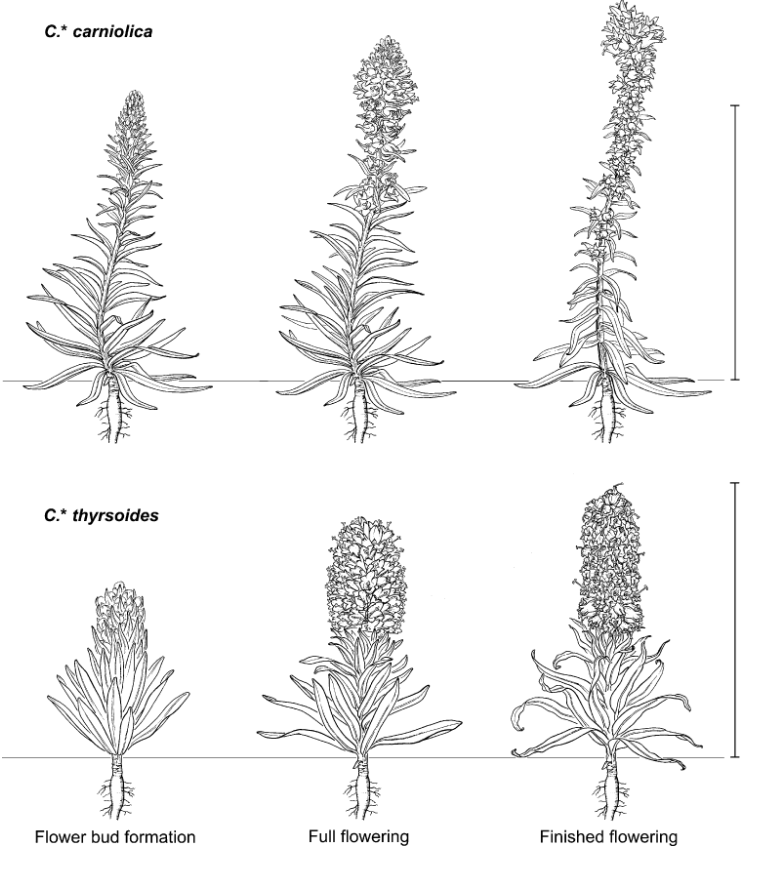
\includegraphics[width=0.7\linewidth]{due_specie.png}
	\caption{\justifying{\footnotesize \textit{\textbf{Morphological difference between \textit{carniolica} and \textit{thyrsoides}.} \footnotesize{The difference between the two subspecies can be mainly attributed to inflorescence height: \textit{carniolica} is usually taller (top). Other differences, as lower Specific leaf area and higher leaf thickness can be attributed to \textit{carniolica} adaptation to drought in the submediterranean climate. Drawing by Atelier Guido K\"{o}hler, Basel. \parencite{scheepensDifferentiationMorphologyFlowering2011}}}}}
	\label{fig:fiori}
\end{figure}

While prior research that had been conducted on the genome size of other European diploid species of  \textit{Campanula} with the same number of chromosomes (\textit{C. garganica, C. latifolia, C. medium, C. portenschlagiana, C. poscharskyana} and \textit{C. pyramidalis}; \cite{zonneveldDNAWeightsNucleus2019}) reported an average DNA weight of $3 pg$, \textit{C. thyrsoides} subsp. \textit{carniolica} shows a bigger genome (N = 13, 2C = 4.944 ± 0.021 pg; \cite{fainelliTaxonomyPlantNursery2025}). DNA weight can be roughly converted to the number of base pairs, where $1 pg = 978 Mbp$ \parencite{dolezelLetterEditor2003} so we could assume \textit{C. thyrsoides} subsp. \textit{carniolica} having genome roughly $4835.2 Mb = 4.83 Gb$ long.

\subsection{Sampling and conservation}\label{sec:SamplesPreparation}
153 fully grown individuals of \textit{Campanula thyrsoides} subsp.  \textit{carniolica} were sampled, collecting 3-4 leaves from each plant between July and August 2022 from 9 locations spanning the North of Italy, South of Austria and West of Slovenia, while the outgrup formed by individuals of \textit{Campanula thyrsoides} subspecies \textit{thyrsoides} were sampled from 2 populations in Italy and France (Figure \ref{fig:map}). 
\begin{figure}[h!]
  \centering
  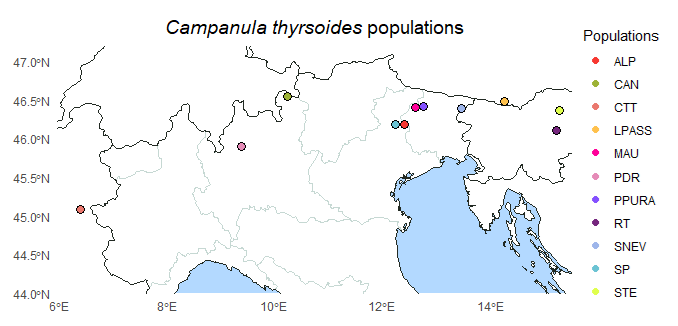
\includegraphics[width=1\textwidth]{map_pol.png}
  \caption{\justifying{\footnotesize \textit{\textbf{Map of sampled populations.} \footnotesize{Populations location over the political map of Italy, France, Slovenia and Austria.}}}}
  \label{fig:map}
\end{figure}
In table \ref{tab:tab1} are reported more information about the location, coordinates and number of samples gathered for each population. A minimum of 15 different individuals sampled per population was attempted, but some populations (i.e. CAN and MAU) weren't big enough. The leaves were stored in bags full of silica to dry, and stored at room temperature (i.e. between 20°C and 25°C) until DNA extraction was performed in 2024.
\begin{table}[h!]
    \centering
    \caption{\textit{Populations' sampling information.}}
    \label{tab:tab1}
    \resizebox{\textwidth}{!}{
    \begin{tabular}{>{\centering\arraybackslash}p{1.5cm} |
                    >{\centering\arraybackslash}p{3cm} |
                    >{\centering\arraybackslash}p{3.5cm} |
                    >{\centering\arraybackslash}p{3cm} |
                    >{\centering\arraybackslash}p{2cm} |
                    >{\centering\arraybackslash}p{2.5cm} |
                    >{\centering\arraybackslash}p{2cm} |
                    >{\centering\arraybackslash}p{1.5cm} |
                    >{\centering\arraybackslash}p{1cm}}

        \toprule
        \textbf{Pop} & \textbf{Locality} & \textbf{Taxon} & \textbf{Region} & \textbf{State} & \textbf{Coordinates} & \textbf{Altitude} & \textbf{Date} & \textbf{N} \\
        \midrule
        CAN & Cancano-Valdidendro Lake & \textit{C. thyrsoides} subsp. thyrsoides & Lombardia & Italy & N 46.5444991 E 10.2547278 & 1960 m & 30/08/22 & 13 \\
        CTT & Col du Télégraph & \textit{C. thyrsoides} subsp. thyrsoides & Auvergne-Rhône-Alpes & France & N 45.0879 E 6.4327 & 2044 m & 30/07/24 & 3 \\
        ALP & Alpago & \textit{C. thyrsoides} subsp. carniolica & Veneto & Italy & N 46.192300 E 12.4156899 & 1140 m & 28/08/22 & 15\\
        MAU & Mauria pass & \textit{C. thyrsoides} subsp. carniolica & Veneto & Italy & N 46.4035951 E 12.6109512 & 860 m & 28/08/22 & 11 \\
        PPURA & Pura pass & \textit{C. thyrsoides} subsp. carniolica & Friuli-Venezia Giulia & Italy & N 46.422130 E 12.752440 & 1320 m & 02/08/22 & 15 \\
        SNEV & Sella Nevea-Chiusaforte & \textit{C. thyrsoides} subsp. carniolica & Friuli-Venezia Giulia & Italy & N 46.3909564 E 13.469300 & 1115 m & 02/08/22 & 15\\  RT & Gračnica-Rimske Toplice & \textit{C. thyrsoides} subsp. carniolica & Savinja Statistical Region & Slovenia & N 46.1111551 E 15.225581 & 245 m & 01/08/22 & 16\\ 
        LPASS & Loiblpass & \textit{C. thyrsoides} subsp. carniolica & Carinzia & Austria & N 46.483864 E 14.261965 & 705 m & 02/08/22 & 16\\
        SP & Serva mountain & \textit{C. thyrsoides} subsp. carniolica & Veneto & Italy & N 46.191773 E 12.243491 & 1590 m & 03/08/22 & 19\\
        STE & Stenica-Vitanje & \textit{C. thyrsoides} subsp. carniolica & Slovenske Konjice & Slovenia & N 46.366841 E 15.281769 & 420 m & 01/08/22 & 15\\
        PDR & Pian dei Resinelli & \textit{C. thyrsoides} subsp. carniolica & Lombardia & Italy & N 45.906065 E 9.394220 & 1290 m & 28/07/22 & 15\\
        \bottomrule
    \end{tabular}
    }
    \caption*{\footnotesize{\textit{Information about populations' sampling, carried out in 2022.}}}
\end{table}
\subsection{Wet lab protocol}
\subsubsection{DNA extraction}
DNA extraction was performed in ((chiedere dove e quando sonpo state fatte le estrazioni)). A total of 153 samples' DNA was extracted following the SILEX: CTAB-Silica protocol illustrated in \autoref{chap:additionalmaterial}. After the extraction, the presence of DNA in each sample is checked by performing several runs on agarose gel 0.8\%: the percentage chosen reflects our expectation of working, at least on this step, with the samples' whole genome. The general rule states that the shorter the DNA fragments are, the higher the percentage of agarose concentration should be preferred, so, to avoid the samples not running properly, we opted for a low density gel. The electrophoresis set up was 90V for 45 minutes.

At each of the following steps, we checked on agarose gel for evidence of the presence of DNA: at this stage it is signalled by a clear band high enough to represent long fragments, which was found in 106 samples out of 153. An example of no strong DNA presence can be seen in Figure \ref{fig:gel}, which shows an 4 samples (in red, RT12, RT13, SP4AI15, SP4B16) that did not show a strong band on the gel: a similar approach will be used, but not thoroughly discussed, in the following sections.

\begin{figure}[h!]
  \centering
  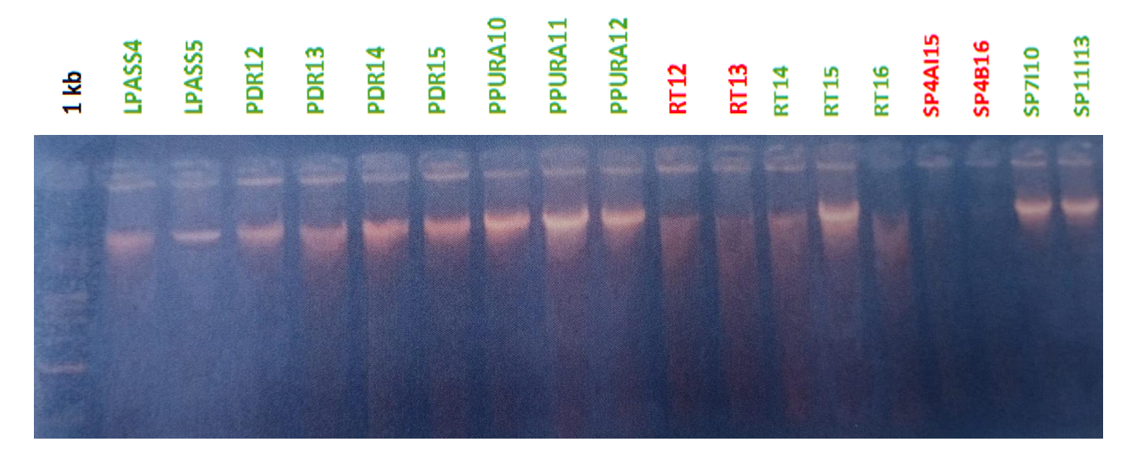
\includegraphics[width=1\textwidth]{gel.png}
  \caption{\justifying{\footnotesize \textit{\textbf{Electrophoresis gel of 18 samples.} \footnotesize{In green, the samples that show a strong band indicating DNA presence, while in red those samples that do not show DNA presence. In black, the ladder used as reference.}}}}
  \label{fig:gel}
\end{figure}

\subsubsection{Digestion}
After the assessment of the presence of DNA, the samples went through digestion which ensures that the DNA is fragmented in pieces of various length, but homogeneous in their distribution. We used a methylation-sensitive endonuclease, ApeKI, that does not cut the sites where cytosine is methylated or regions full of repetitive sequences \parencite{sonahImprovedGenotypingSequencing2013}, which is usually where DNA is silenced. By ensuring that those fragments aren't part of the sequences included in the study, we focused on highly indicative DNA sequences, while reducing cost. This is not the only advantage of the use of ApeKI: it also cuts DNA in precise restriction sites, leaving so called 'sticky ends' at the extremes of the fragments (Figure \ref{fig:apeK1}). The reads will contain a CWG sequence (where W is either an A or a T), which is useful when building proper adapters for the next steps.

\begin{figure}[h!]
  \centering
  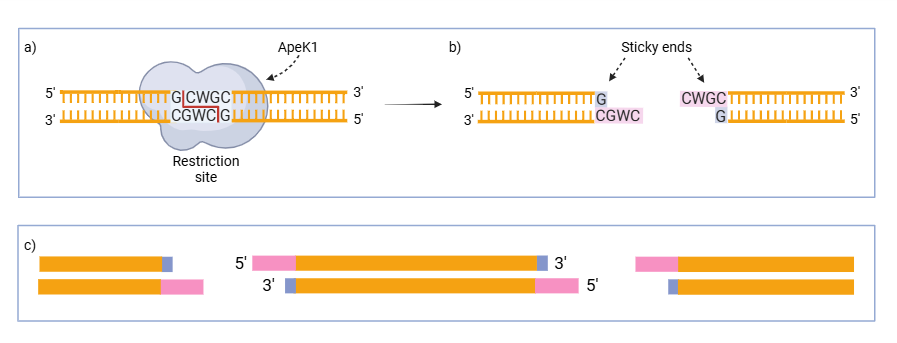
\includegraphics[width=1\textwidth]{ApeK1 restriction site.png}
  \caption{\justifying{\footnotesize \textit{\textbf{ApeKI restriction site and action.} \footnotesize{a) ApeKI restriction site CWG. b) Creation of sticky ends on DNA fragments. c) Several fragments of dsDNA. Created in  https://BioRender.com}}}}
  \label{fig:apeK1}
\end{figure}

To digest the same amount of DNA (50 ng) for each sample, the samples were diluted with $ddH_2O$ accordingly to their concentration, until desired volume ($44 \mu L$), to which $2 \mu L$ of ApeKI and $4 \mu L$ of NEB r3.1 10x buffer are added. More information about the protocols used for digestion and adapters preparation can be found in \autoref{chap:additionalmaterial}.

\textit{Campanula thyrsoides}, though, proved to be hard to digest, and the samples as tested on the agarose gels (between 1 and 1.5\%, run at 85V for 60 minutes) did not show an homogeneous smear typical of a complete digestion: this was probably due to the high content of latex in the leaves \parencite{kussBiologicalFloraCentral2007}. To improve digestion, we decided to test different variation of the traditional protocol, already used to digest tomatoes (\textit{Solanum lycopersicum}) in the same laboratory, that called for a 2 hours incubation time with reagents at 75°C. After using this protocol on a subset of samples (ALP1 to ALP11) , we tried three different possible solutions:
\vspace{-1.2em}
\begin{enumerate}
\setlength\itemsep{-0.3em}
    \item first we simply increased the incubation time to 4 hours;
    \item the second time we used a 4 hours incubation time, added an additional $2 \mu L$ of ApeKI and $4 \mu L$ of r3.1 10x buffer and left the samples incubate 8 hours overnight;
    \item the third, and last time, we left the sample to incubate for a total of 12 hours (original 4 hours, plus 8 overnight) at 75°C without adding additional reagents.
\end{enumerate}
We noticed that the homogeneity of the smear on agarose gel improved slightly when leaving the gel incubate overnight, but did not show any remarkable difference with the use of additional reagents. At this step, samples that did not show any nucleic acid material in the agarose gel were discarded from the library preparation: the whole population of Cancano (CAN) and 34 other individuals had to be scrapped - in Table \ref{tab:digestion} they are crossed out with a line.

\subsubsection{Ligation}\label{ligation}
During ligation, the reads of the samples that weren't discarded in the previous step, are ligated with adapters that can either be indexed or not, depending on the sequencing method employed. We used double indexed adapters, necessary for Illumina TruSeq combinatorial-dual DNA sequencing: in Figure \ref{fig:library} the barcodes (4 to 8 bp long) present only on the forward read are highlighted in blue, the indexes in sky blue and the Truseq adapters are shown in red/orange. Both the barcoded and common adapters are present in the same solution (called stock solution) produced during adapters preparation. More information about the preparation of the stock solution and the ligation protocol can be found on Additional Materials, \autoref{chap:additionalmaterial}. 

\begin{figure}[h!]
	\centering
	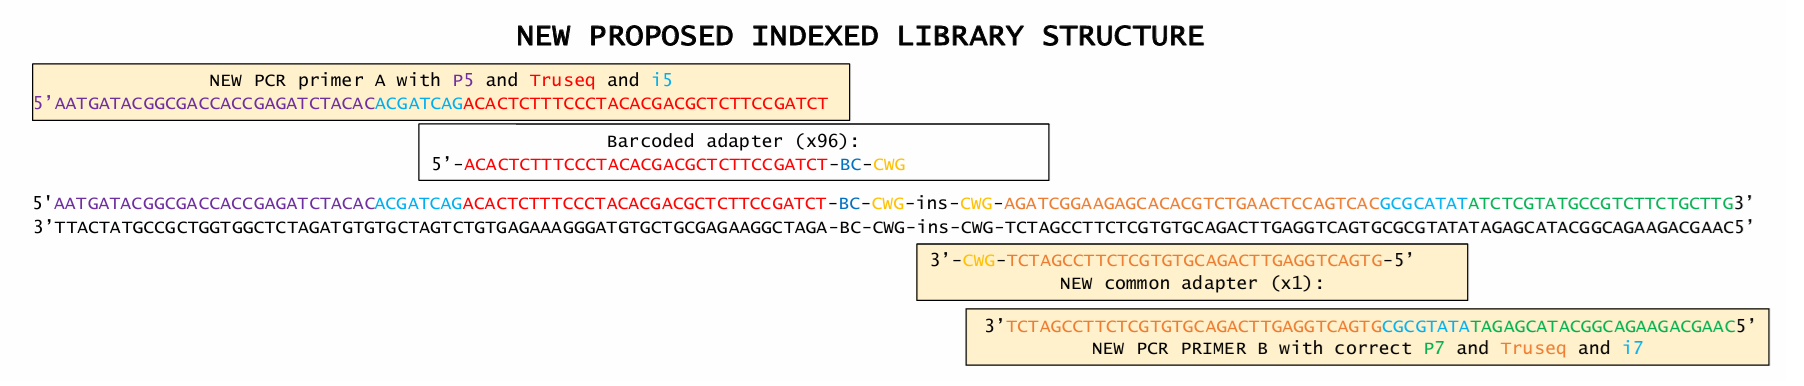
\includegraphics[width=1\linewidth]{library.png}
		\caption{\justifying{\footnotesize \textit{\textbf{Library structure.} \footnotesize{In blue the barcode (labelled as "BC") which univocally identifies each sample: the barcode is only ligated to the forward read and the complete list can be found in Table \ref{tab:barcodes}. In red and orange Truseq adapters (sequencing primers), and in light blue the i5 and i7 Illumina library indexes. In purple and green the P5 and P7 adapters, that facilitate clonal amplification and sequencing reactions. Lastly, in yellow, the restriction sites where ApeKI cuts the insert, here labelled as "ins".}}}}
	\label{fig:library}
\end{figure}

\subsubsection{Pooling and amplification}
After ligation fragments were amplified using Monarch PCR and cleaned using Monarch DNA cleanup kit to produce the sequencing library (the full protocol can be found in the Additional Materials chapter).  PCR amplification requires that forward P5 primer and reverse P7 primer (in Fig. \ref{fig:library} in purple) are also attached, respectively on the 5' and 3' end of the reads. After this step the library was quantified with Qubit station (we obtained a concentration of $60 \ ng/\mu L$) and the fragments size was checked with Tapestation. GBS protocols usually do not involve a direct size selection prior to PCR \parencite{elshireRobustSimpleGenotypingbySequencing2011} \parencite{sonahImprovedGenotypingSequencing2013}, libraries are only checked to ensure that the majority of the fragments are in the correct size range. With subset ALP1-ALP11 we followed the standard workflow, but with the second sequencing batch (from ALP12 to the end) we've noticed that fragments were showing peaks out of our target of 200-500 bp length. The one at around 25bp and the other at 1500bp are expected, since they are used by the Tapestation as reference, while our sample showed fragments between 500 to 1000 bp of length, which are not ideal (Figure \ref{fig:sizesel}, a). To improve our library before sending it to sequencing, we used Sera-Mag Select Size Selection kit from cytiva, employing Dual-Side size selection between 150 to 500 bp, with an average size of 250 bp: this paid off, and Tapestation showed only one peak between 200 and 500 bp of length  (Figure \ref{fig:sizesel}, b). Size selection's protocol is reported in the appropriate section in Additional Materials.

\begin{figure}[h!]
	\centering
	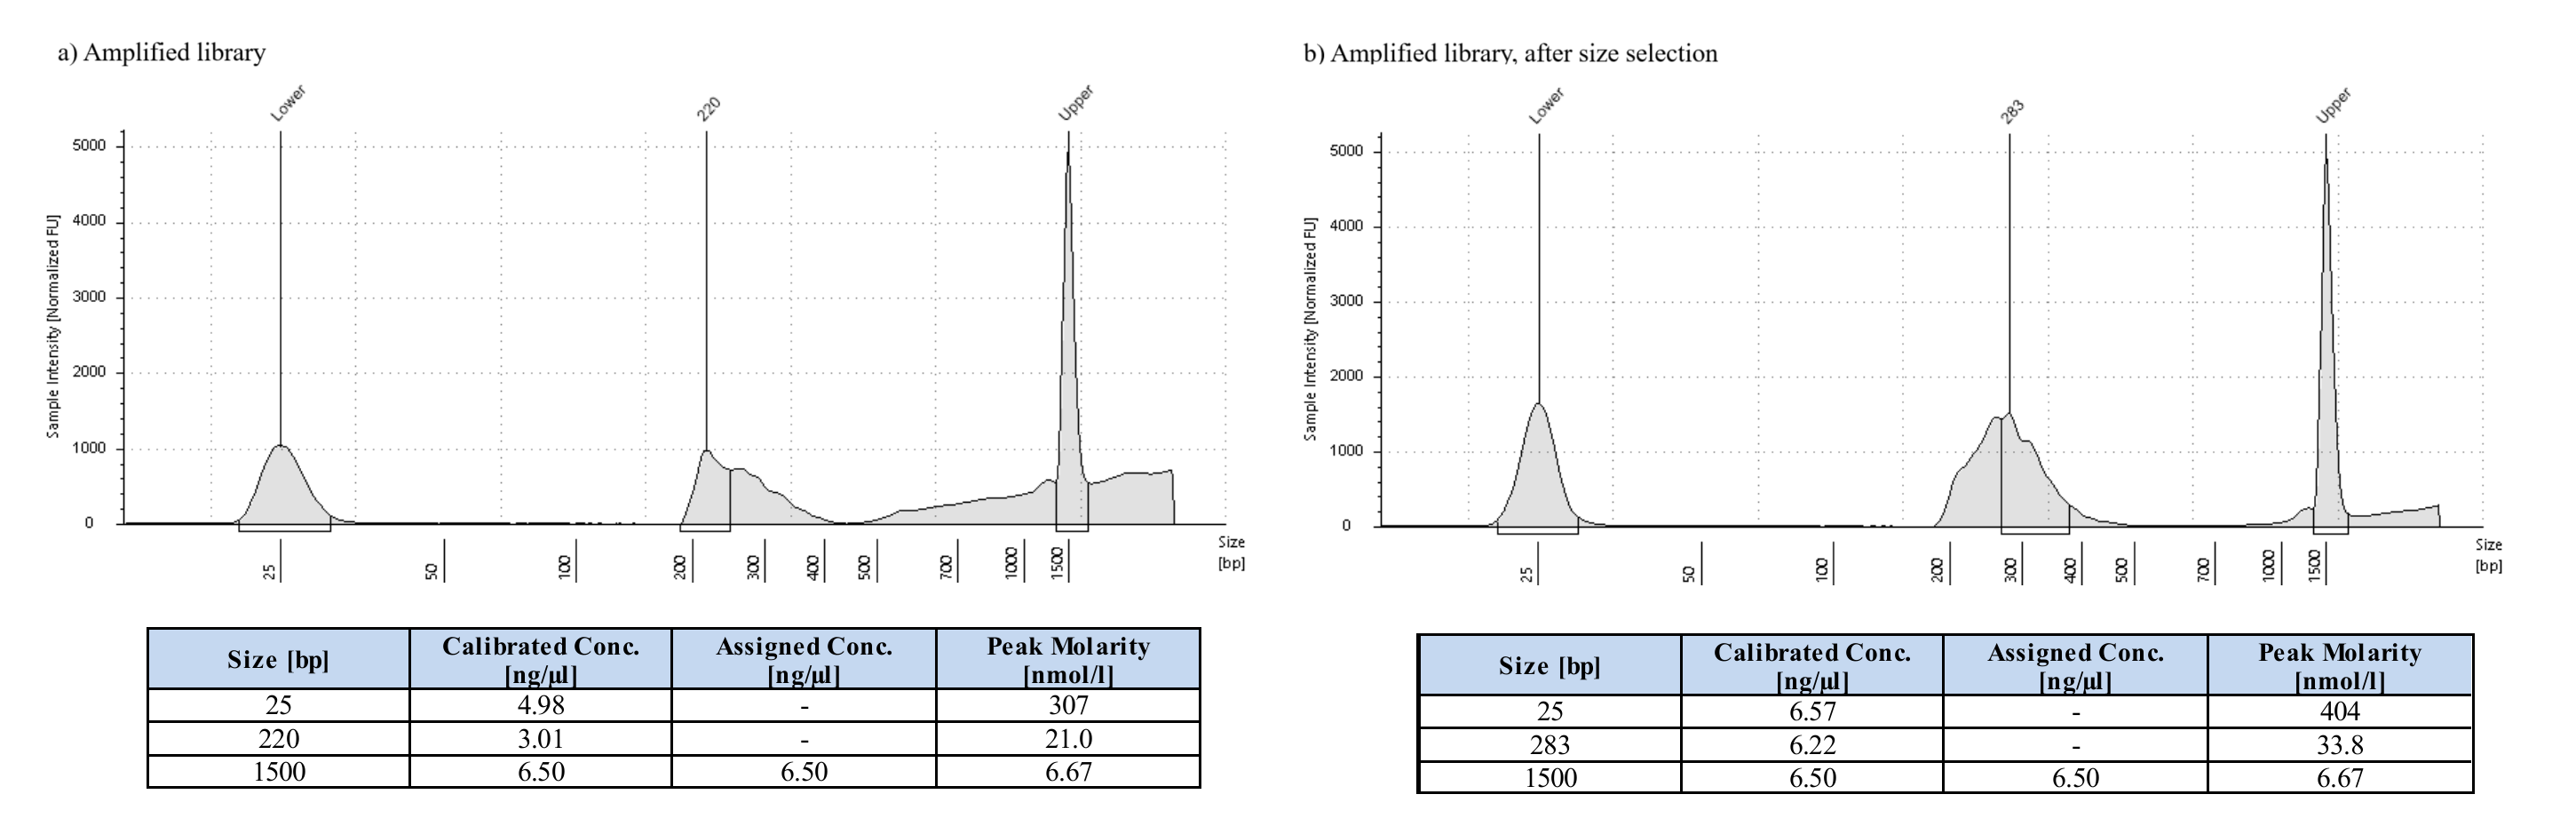
\includegraphics[width=1.03\linewidth]{before_vs_after_sizesel.png}
	\caption{\justifying{\footnotesize \textit{\textbf{Library before and after size selection.} \footnotesize{Reads length distribution in the library before (a) and after (b) size selection: on the y axis the sample intensity, and on the x axis the fragments length in base pairs. A table with peaks' concentration and molarity information is also added on the bottom of each plot.}}}}
	\label{fig:sizesel}
\end{figure}

\subsection{DNA sequencing}
 Initially, a subset of 10 samples (ALP1-ALP11) were sent to GENEWIZ from Azenta Life Sciences (Leipzig, Germany) for sequencing in January 2025, then the remaining 96 were sent in April 2025: standard Illumina TruSeq combinatorial-dual DNA sequencing was used for both sequencing batches and sequences' data was received in \texttt{.fastq} format shortly after submission.
 
\subsection{The bioinformatics pipeline}

All the projects mentioned in this thesis followed the same pipeline (Figure \ref{fig:pipeline}), which was built on the objective of the main project, namely the reconstruction of \textit{Campanula thyrsoides} subspecies \textit{carniolica} populations' structure. The secondary projects differ from it by just the choice of starting and/or ending step, as well as some of the parameters used. These discrepancies are thoroughly explained in each project's section.

\begin{figure}[h!]
	\centering
	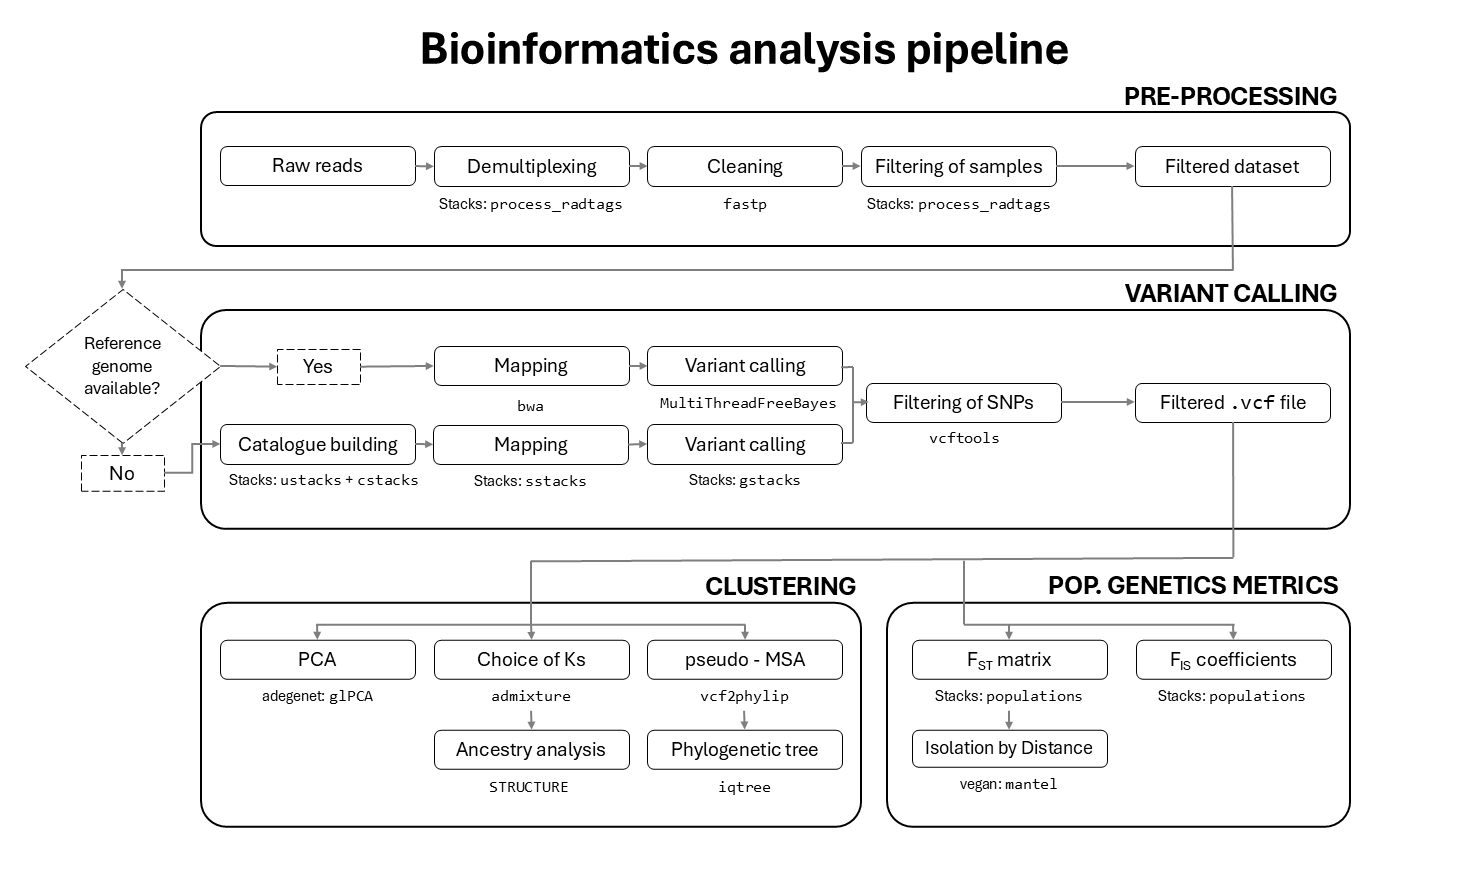
\includegraphics[width=1\textwidth]{pipeline.png}
	\caption{\justifying{\footnotesize \textit{\textbf{Bioinformatics analysis' pipeline.} \footnotesize{Full pipeline followed in all the projects, except for a few adjustments in parameters chosen. The function used at each step is shown undereneath it, as well as the software or R library it belongs to, if the name differs.}}}}
	\label{fig:pipeline}
\end{figure}

\subsection{Pre-processing}
Individuals from ALP1 to ALP11 were sequenced in a different batch than the other samples. Considering the time that passed before receiving the second batch of data, samples ALP1 to ALP11 were used as a subset to test some of the tools employed in the pipeline, and underwent pre-processing separately from the second batch (ALP12 onward). 

\subsubsection{Demultiplexing and quality checks}
Demultiplexing, namely the process of separating the DNA sequences depending on the samples they come from, is based on the barcode attached to it during the ligation step (\autoref{ligation}).  For this step, a custom script was written (\texttt{01\_demultiplex.sh}) which runs the command \texttt{process\_radtags} from software Stacks (version: 2.68; \cite{catchenStacksBuildingGenotyping2011}) and collects all the unpaired sequences in one folder. It takes as input a compressed file in \texttt{fastq} format which contains all the sequences, the name of the restriction enzyme used (ApeKI) and finally a text file containing sample and barcode couples. This step not only separates the sequences but also removes the barcode from the forward read; the full list of samples accompanied by their barcodes (table \ref{tab:barcodes}) can be found in the Additional Materials chapter. 

\subsubsection{Trimming using fastq-mcf and fastp}
After separating them, all the sequences were cleaned, a loose term which encompasses several operations:
\vspace{-1.5em}
\begin{itemize}\setlength\itemsep{-0.2em}
	\item Eliminate the Illumina adapters contamination;
	\item Trim low quality scores sequences sections. Quality is denoted by Phred-score (q), calculated as \parencite{ewingBaseCallingAutomatedSequencer1998}:
	\begin{equation}
		q = -10 \cdot log_{10}(p) 
	\end{equation}
	where p is the estimated error probability for that base-call. Phred quality scores that are less
	than 30 are considered unreliable \parencite{oraweAccountingUncertaintyDNA2015};
	\item Trim poly-G tails. These artifacts of repeated, high-confidence Guanine bases appear on two-channel sequencing systems when the signal is too weak to be detected, and is erroneously recognized as a G in the base calling stage;
	\item Finally, after trimming, discard the sequences that are shorter than 50 base-pairs.
\end{itemize}
\vspace{-1.5em}
Two different softwares were tested on the ALP1-ALP11 subset to determine the most efficient tool; \texttt{fastq-mcf} (v1.05; \cite{aronestyEautils2011}) and \texttt{fastp} (v0.24.0; \cite{chenFastpUltrafastAllinone2018}). The performance was evaluated in terms of computational time, quality of cleaning and number of reads retained on average. Ultimately, the latter was chosen as the cleaning tool for the second batch of samples too and used in a custom script (\texttt{02\_trim\_fastp.sh}), which automatizes the process by iterating the command through all the samples. \texttt{fastp} also requires a \texttt{fasta} file which contains the Illumina adapters sequences to remove from within the reads: the list also included sequences of adapters containing the barcodes used during the demultiplexing step, as it was noticed that some reverse reads still contained them.

\subsection{Variant calling}\label{variant-calling}
Variant calling, which aims to identify single-nucleotide polymorphisms (SNPs) in the sample's DNA, is usually performed by aligning to a reference genome. To account for the fact that \textit{Campanula thyrsoides} lacks a reference genome for its nuclear DNA, the pipeline \texttt{denovo\_map.pl} from Stacks was employed: such tool is able to identify loci \textit{de novo} and calls genotypes using a maximum likelihood statistical model \parencite{catchenStacksBuildingGenotyping2011}.

\subsubsection{Stacks: denovo\_map.pl pipeline}
\texttt{denovo\_map.pl} is a modular pipeline that runs six different components of Stacks: in order, it calls \texttt{ustacks}, \texttt{cstacks}, \texttt{sstacks}, \texttt{tsv2bam}, \texttt{gstacks} and lastly \texttt{population} (Figure \ref{fig:pipeline_denovo}). The pipeline takes as input a dataset of demultiplexed and cleaned reads, a population map and the following parameters:
\vspace{-1.5em}
\begin{description}\setlength\itemsep{-0.2em}
	\item [m: ] in \texttt{ustacks}, the minimum number of reads to create a stack (default 3, figure \ref{fig:pipeline_denovo}, A to B);
	\item [M: ] in \texttt{ustacks}, the maximum distance, in nucleotides, allowed between stacks (default 2, figure \ref{fig:pipeline_denovo}, C to D);
	\item [n: ] in \texttt{cstacks}, the number of mismatches allowed between stacks of different individuals to be merged into one (default is set equal to \textbf{M}, figure \ref{fig:pipeline_denovo}, F).
\end{description}
\vspace{-1.5em}

\begin{figure}[h!]
	\centering
	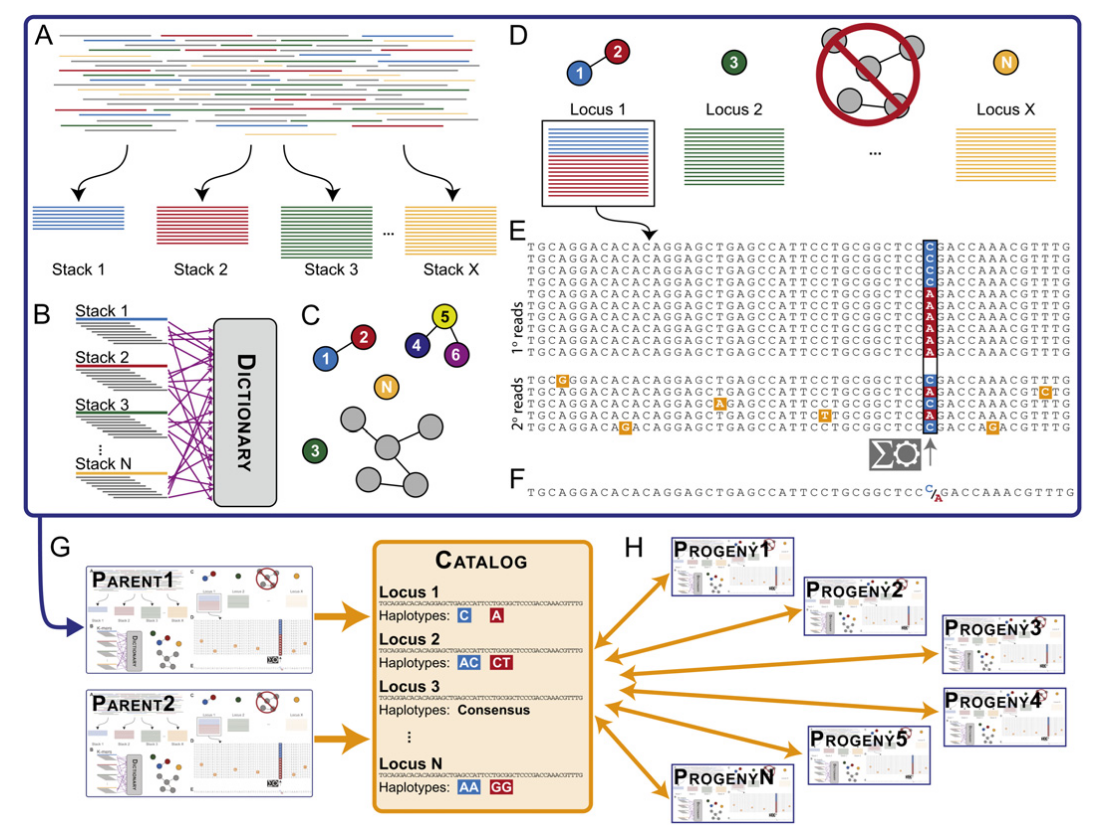
\includegraphics[width=0.7\textwidth]{denovo_pipeline.png}
	\caption{\justifying{\footnotesize \textit{\textbf{Stacks: \texttt{denovo\_map.pl} pipeline.} \footnotesize{Full view of the Stacks: \texttt{denovo\_map.pl} pipeline from Catchen \textit{et al.} (2011) \parencite{catchenStacksBuildingGenotyping2011}. It starts with (A) \texttt{ustacks}, which, for each individual, forms stacks of minimum $m$ reads that match exactly, (B) breaks down each stack into k-mers and stores them in a dictionary (C). Then matches secondary reads (D) based on a certain number $M$ of mismatches to increases stack depth. Each locus at each nucleotide position is checked for polymorphisms and a consensus sequence is called (E). (F) \texttt{cstacks} then loads all stacks into a Catalog to create a set of all possible loci, merging those that have at maximum $n$ mismatches between each other. (G) \texttt{sstacks} matches map cross progeny against the Catalog to determine the haplotypes at each locus in every individual in the cross. \texttt{populations}, at the end, computes genetic populations metrics based on the SNPs called and a population map provided.}}}}
	\label{fig:pipeline_denovo}
\end{figure}

The population map is a text file that associates each sample to its population of origin: it is used solely to optimize the number of polymorphic loci found in a certain percentage of the individuals of each population. This allows to discard uninformative loci from the final matrix. Other filtering methods that consider all samples dataset in its entirety are employed in the next steps.

\subsubsection{Monte Carlo and Taboo Search for hyperparameters' tuning}
To optimize the parameters for \texttt{denovo\_map.pl}, a variation of the r80 method \parencite{parisLostParameterSpace2017} was employed. In the classical r80 method, the parameters are selected depending on which ones maximize the number of polymorphic loci in at least 80\% of the individuals of the study, hence the name. The percentage could be changed depending on how strict the user of the pipeline wants to be (increase in percentage equals a stricter selection), but Paris \textit{et al.} (2017) found that 80\% was the optimal percentage for a good trade-off between quality and quantity of loci found. The change we introduced was that the performance of the parameters was evaluated not only on the number of polymorphic loci found but also on a minimum of mean coverage obtained over all the samples, and on the number of unique, independent SNPs (counting only one SNP for each locus to reduce the effect of linkage disequilibrium). 

To perform the search of the optimal parameters, performed on the ALP1-ALP11 subset, we first defined a search space for the parameters we wanted to test. The ranges of tested parameters were set, after an initial quick assessment of the proposed ones in Paris \textit{et al.} (2017), as 3 to 5 for m and 0 to 4 for both M and n. Then two custom scripts were prepared: \texttt{gen\_random\_pop.sh} which randomly generates a set of parameters from the ranges defined in the search space, checks if it was already explored (not present in a \texttt{log\_combinations.txt} file), calls the Stacks: \texttt{denovo\_map.pl} pipeline and then executes the second custom script \texttt{add\_to\_log.sh}. This last script extracts some information from the log file of the pipeline such as mean and standard deviation of read coverage, the number of total loci, the number of SNPs per locus and adds a FAIL flag to determine if that combination fails some minimum requirements. Only loci that were genotyped in at least 80\% of the samples were selected for further analysis ($r = 0.80$), minimizing missing data. Crucially, for this parameters search, the $r = 0.80$ flag was used as to apply the filter to the whole dataset, although in \texttt{Stacks:} \texttt{populations} SNPs are selected based on the percentage of missing data in each population. In our case, our subset ALP1-ALP11 is part of the same population, so the two filters overlap, but when tuning on a bigger dataset, we recommend using a temporary population map which places all samples in the same population, even if they actually belong to different populations. 

This parameters search can be seen as a Taboo restricted Monte Carlo search. A Monte Carlo method is essentially a technique that gathers information about a random object (in our case, the parameters' performance on the pipeline) by observing random realizations of it \parencite{kroeseWhyMonteCarlo2014}: we exploit this method by randomly generating parameters combination and testing them. During each iteration of a simple Taboo search, on the other hand, a subset of \textit{taboo moves} is created out of all the possible ones, and membership to this group is determined by a set of taboo conditions (i.e. a logical relationship; \cite{gloverTabuSearchPart1989}). In this case a combination enters the subset of taboo moves simply if it was already explored. Any algorithm usually stops after either a chosen number of iteration has elapsed in total or since the solution as explored: we decided to stop after $n = 45$ combinations were explored. Each combination $i$ is the evaluated with a custom-prepared scoring function, that assigns the following score ($s$):
\begin{equation}\label{eq:score}
	s_i = 
	\frac{
		\dfrac{\text{tot SNPs}_i}{\text{tot unique loci}_i}
	}{
		\displaystyle \max_{n} \left( \dfrac{\text{tot SNPs}_n}{\text{tot unique loci}_n} \right)
	}
	+
	\frac{
		CV_i
	}{
		\displaystyle \max_{n} \left( CV_n \right)
	}
	+
	FAIL_i
	-
	\frac{
		\text{tot unique loci}_i
	}{
		\displaystyle \max_{n} \left( \text{tot unique loci}_i \right)
	}
\end{equation}
\noindent \textbf{Where:}
\begin{equation}
	FAIL_i = f(x) =
	\begin{cases}
		5, & \text{if } \text{unique loci}_i < 2400 \text{ or } \mu_{\text{coverage}_i} < 10 \\
		0, & \text{otherwise}
	\end{cases}
\end{equation}
The best set of parameters has the minimum score $s$ out of all the explored ones. This equation ensures:
\vspace{-1.5em}
\begin{itemize}\setlength\itemsep{-0.2em}
	\item a \textbf{penalty} for each locus that contains more than one SNP (first term), which would mean that they are in linkage. This quantity is normalized over all the explored combinations to not skew the scores;
	\item a \textbf{penalty} for average coverage with a large standard deviation across samples (second term), normalized over all the explored combinations as well. To ensure that an higher average coverage would not be penalized by a predictably big, in absolute values, standard deviation, we did not penalize the standard deviation itself, but instead the coefficient of variation ($CV$). $CV$ for a combination $i$ is computed as:
	\begin{equation}
		CV_i = \frac{\sigma_{\text{coverage}_i}}{\mu_{\text{coverage}_i}}
	\end{equation}
	\item a \textbf{penalty}, which also meant an instant \textbf{fail} thanks to the sum of 5 points to the score, to those combinations which did not reach a minimum of average 10x coverage and/or did not find at least 2400 loci. This third term of the equation ensures that no values lower than these are accepted, because they would not be enough for a strong statistical analysis, since SNPs are filtered on the next steps and are only bound to decrease. These values can be changed on a case-by-case basis: the average coverage could be set higher for a stricter selection (we would not recommend a lower value) while the minimum number of loci found should be raised with the number of samples provided;
	\item finally, a \textbf{reward} to combinations that resulted in an higher number of loci (fourth term), normalized over all the combinations.
\end{itemize}
\vspace{-1.5em}
This edit in the r80 method ensures a stricter evaluation of parameters aimed at the optimization of different outputs of the pipeline: this aids the statistical strength of the next analyses, while retaining an overall simplicity in its application. 

\subsubsection{Filtering out SNPs}

After performing hyperparameters' tuning on the ALP1-ALP11 subset, we used \texttt{denovo\_map.pl} with parameters $m = 4$, $M = 1$ and $n = 1$ on the whole dataset. The output of this step was a standard \texttt{.vcf} file containing called SNPs and their positions, except for the fact that, since they were called on a catalog of stacks and not on a reference genome, the "chromosome" section showed sequentially increasing numbers according to the numerical ID of the stack. The file was later filtered using \texttt{vcftools} (v0.1.16; \cite{danecekVariantCallFormat2011}) with the following parameters:
\vspace{-1.5em}
\begin{itemize}\setlength\itemsep{-0.2em}
	\item \textbf{max-missing 0.9}: While the r80 filter in the \texttt{Stacks:} \texttt{denovo\_map.pl} ensures that SNPs are retained if present in at least 80\% of  each populations, \texttt{vcftools} instead filters out those with more than 10\% of missing data through the whole dataset. This ensures we retain only real polymorphic loci and not those whose information is only the presence or absence of the called SNP;
	\item \textbf{min-meanDP 5}: Includes only sites with average depth values (over the whole dataset) greater than 5, based on the "DP" tag in the \texttt{.vcf} file;
	\item \textbf{thin 1000}: retains only one SNP every 1000 base pairs, to ensure independence of SNPs, assumption on which we operate. The more genetic markers in a study, the more of them are required to be independent in order to assign an individual to a certain sample pool with known allele frequencies (a population genetics principle used already in forensic identification; \cite{visscherLimitsIndividualIdentification2009}). SNPs that assort independently are said to be unlinked, and have a recombination frequency of 50\%, and the higher the frequency of recombination between two markers, the further away they are situated on a chromosome \parencite{semagnPrinciplesRequirementsProspects}. There are two formulas that can be used to find the map distance $d$ in cM between two loci, depending on their recombination rate $R$: Haldane's (\ref{haldane}) and Kosambi's (\ref{kosambi}) \parencite{huehnRandomVariabilityMap2010}.
	\begin{equation}\label{haldane}
		d_H = 
		\begin{cases}
			-0.50 \cdot \ln \left( 1-2R \right), & \text{for } R < 0.50\\
			\infty, & \text{for } R = 0.50
		\end{cases}
	\end{equation}
	\begin{equation}\label{kosambi}
		d_K = 
		\begin{cases}
			0.25 \cdot \ln \left( \frac{1 + 2R}{1 - 2R} \right), & \text{for } R < 0.50\\
			\infty, & \text{for } R = 0.50
		\end{cases}
	\end{equation}
	
	In theory, these formulas could be used to assess a minimum distance between SNPs to have no linkage or a partial one. When two loci are located on the same chromosome they can never be truly unlinked, since these functions possess a vertical asymptote at $R = 0.5$ (Figure \ref{fig:haldane-kosambi}).
	 Only two loci located on different chromosomes are truly independent since they cannot physically recombine: their recombination rate is arbitrarily set to 50\% and their distance cannot be computed. We could consider independent those loci with a suppressed recombination rate ($R_i < average(R)$) \parencite{semagnPrinciplesRequirementsProspects}, but in order to compute that, a genome-wide genetic mapping of \textit{Campanula thyrsoides} would be needed. Since there is no reference genome available for this species, we could not compute the average recombination rate, nor we could assess the SNPs location on a chromosome: our only information is about the locus position on a certain stack. By requesting a minimum distance of 1000 bp between SNPs, we could filter out SNPs on the same stack: they are built using reads with a median length of 100 bp, so a distance of 1000 bp is enough to ensure picking one SNP per stack.
	 
	 \begin{figure}[h!]
	 	\centering
	 	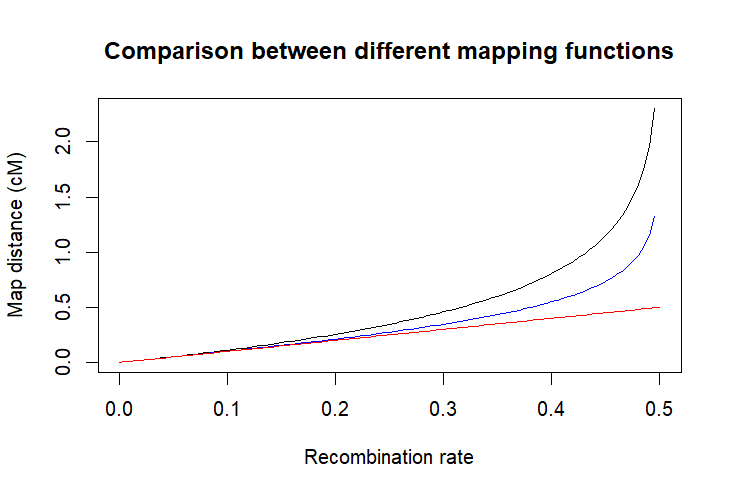
\includegraphics[width=0.7\textwidth]{haldane_kosambi.png}
	 	\caption{\justifying{\footnotesize \textit{\textbf{Comparison of Haldane’s and Kosambi’s mapping functions.} \footnotesize{The red line shows a linear relationship between map distance (in cM) and recombination rate ($R$), while the black and the blue one show how the map distance grows exponentially with the recombination rate following, respectively, Haldane's (\ref{haldane}) and Kosambi's (\ref{kosambi}) functions. Haldane's assumes there no interference, namely the effect of a crossover in one region on the likelihood of a crossover in another one \parencite{huehnRandomVariabilityMap2010}. there is no direct linear relationship between units of genetic distances in centimorgan (cM) and physical distances in kilobase pairs (kb), and depends solely on the organism in the study \parencite{semagnPrinciplesRequirementsProspects}.}}}}
	 	\label{fig:haldane-kosambi}
	 \end{figure}
	\item \textbf{maf 0.005}: Include only sites with a Minor Allele Frequency greater than 0.005. It is defined as the number of times an allele appears over all individuals at that site, divided by the total number of non-missing alleles. The minimum $maf$ we use as threshold is computed as:
	\begin{equation}\label{formula:maf}
		maf_{threshold} = \frac{1}{\text{number of alleles} \cdot \text{number of samples}} = \frac{1}{2 \cdot 103}
	\end{equation}
	This metric helps to distinguish between common and uncommon SNPs in a population: the loci with low MAF have limited heterozygosity and are thus less informative. MAFs lower than 0.5\% usually refers to SNPs that describe rare variants behind, for example, uncommon diseases \parencite{kanakaConceptsMeasuresDiversity2023} in a specific individual. Our study objective is a population-wide analysis, so SNPs that refer only to a variant in a single, or a small group of individuals can be discarded. Furthermore, most novel (initially rare) alleles arising through mutation are deleterious and could have negative impacts: this means that they should not be targets for conservation \parencite{whitlockConsequencesInsituStrategies2016}.
\end{itemize}
\vspace{-1.5em}

\subsection{Population genetics analyses}
After obtaining the genotype at each locus where a SNP is found, this information can be used for a series of analyses: metrics for a quantitative analysis of the genetical structure of the populations and different clustering methods to individuate their belonging to bigger groups or a subdivision in smaller subpopulations. We are going to talk about each method to perform these analyses in detail, reserving the results and discussion to the appropriate chapters.

\subsubsection{Metrics}
To determine the genetical structure of the populations in a quantitative way, the most common used metrics are those defined by Wright \parencite{wrightGeneticalStructurePopulations1949} as different fixation indexes. Assuming that the total putative original population is called $T$, each subpopulation deriving from its subdivision is referred as $S$ and is formed by individuals $I$, we can define:
\vspace{-1.5em}
\begin{description}
	\item[\textbf{$F_{IS}$}] - The inbreeding index that is most used in literature, called by Wright (1949), "current inbreeding coefficient". It can be computed as:
	\begin{equation}
		F_{IS} = 1 - \dfrac{H_{ob}}{H_{exp}} = 1 - P_{IS}
	\end{equation}
	where $H_{exp}$ is the expected heterozigosity within the same subpopulation assumed generated by random mating, $H_{ob}$ is the observed heterozigosity and $P_{IS}$ is the panmictic index associated to $F_{IS}$. This is the only index that can be estimated from frequency of data of a single population \parencite{weirEstimatingFStatisticsAnalysis1984} and ranges from -1 to 1, were -1 describes a population of individuals different from each other and 1 is associated to a population composed by fixed lines. We computed this value using R package \texttt{hierfstat};
	\item[\textbf{$F_{IT}$}] - This index is defined as the version of $F_{IS}$ which is computed for individuals relative to the total, and it is what Wright defines as, simply,  "inbreeding coefficient". A clearer definition of this is given by Weir and Cockerman in 1984 \parencite{weirEstimatingFStatisticsAnalysis1984}, as the correlation of genes within individuals of the full population. Differently from $F_{IS}$, $F_{IT}$ depends on the population's ($T$) size and history so it needs the information given by all the individuals ($I$) in the dataset \parencite{weirEstimatingFStatisticsAnalysis1984}. It is unaffected, though, by the number of alleles sampled, the number of individuals within subpopulations ($S$) and the number of subpopulations themselves. Similarly to $F_{IS}$, $F_{IT}$ ranges from -1 to 1 and its interpretation reflects the same as the former and it can also be associated with a panmictic index $P_{IT} = 1 - F_{IT}$ \parencite{wrightGeneticalStructurePopulations1949}.;
	\item[\textbf{$F_{ST}$}] - Defined by Wright (1949) as the "correlation of randomly drawn gametes from the same population, relative to the total population", it is calculated as:
	\begin{equation}\label{wright}
		F_{ST}^W = \dfrac{F_{IT}-F_{IS}}{1-F_{IS}} = \dfrac{P_{IT}}{P_{IS}}
	\end{equation}
	$F_{ST}$ is strictly positive, with values ranging from 0 to 1, where 0 quantifies a little difference between subpopulations and 1 a strong difference between them. However, Wright did not specify what is the total population, so different authors interpreted it in different manners. While for Nei (1973) it is the combination of the two population samples, for Cockerman (1969) and Weir and Hill \parencite{weirEstimatingFStatistics2002}, the total population is the most recent common ancestral population to the two subpopulations being considered. In synthesis, the former viewed $F_{ST}$ as a statistic from observed samples, which varies according to the number of sub populations observed \parencite{weirEstimatingFStatisticsAnalysis1984}, while the others as a parameter of the evolutionary process \parencite{bhatiaEstimatingInterpretingFST2013}. For this reason Weir and Cockerman (1984) define $F_{ST}$ also as "coancestry", and compute it as: 
	\begin{equation}\label{WC}
		F_{ST}^{WC} = 1- 
		\dfrac{
			2 
			\cdot
			\dfrac{n_1n_2}{n_1+n_2} 
			\cdot
			\dfrac{1}{n_1+n_2-2}
			\cdot
			[n_1p_1(1-p_1)+n_2p_2(1-p_2)]
		}
		{
		\dfrac{n_1n_2}{n_1+n_2}(p_1-p_2)^2
		+
		\left ( 2 \cdot 
		\frac{n_1n_2}{n_1+n_2}-1
		\right )
		\dfrac{1}{n_1+n_2-2}
		[n_1p_1(1-p_1)+n_2p_2(1-p_2)]
		}
	\end{equation} where $n_i$ is the population $i$ sample size and $p_i$ is its allele frequency. If the sample sizes are unequal, the estimate will depend upon the ratio of sample sizes: this makes $F_{ST}^{WC}$ not comparable across studies with different sample sizes. It is possible to correct this estimate considering the ratio of sample sizes, but another, more direct method, was proposed in 2002 by Weir and Hill \parencite{weirEstimatingFStatistics2002} which introduced population-specific estimates of $F_{ST}$ that is not influenced by the aforementioned limitation. Assuming $p_i^s$ allele frequency of the derived allele in population $i$ at SNP $s$ and $p_{anc}^s$ the allele frequency of the derived allele in the ancestral population at that SNP position, Weir and Hill define the following relationship between them:
	\begin{equation}
		\mathtt{E}[p_i^s | p_{anc}^s] = p_{anc}^s
	\end{equation} 
	for those SNPs that were already present in the ancestral population, and are not derived from a recent mutation. The variance present in the studied sample of the population $i$ is then used to calculate the population-specific $F_{ST}^i$ for a specific SNP $s$ as:
	\begin{equation}\label{WH}
		F_{ST}^{WH, i} =  \dfrac{Var(p_i^s | p_{anc}^s)}{p_{anc}^s(1-p_{anc}^s)}
	\end{equation}
	Estimates of $F_{ST}$ across multiple SNPs can be combined, but this can be done in two different ways: either first averaging the two components of equation \ref{WH} and then calculating the ratio ("ratio of averages" \parencite{bhatiaEstimatingInterpretingFST2013}), or averaging genome-wide the single SNP estimates ("average of ratios"). Different softwares use distinct approaches, although the first method will converge to the correct underlying value as the number of independent SNPs increases, so it is the most recommended \parencite{bhatiaEstimatingInterpretingFST2013}.
	For two populations, the quantity is simply an average of the two population-specific $F_{ST}$ values:
	\begin{equation}
		F_{ST}^{WH} = \dfrac{F_{ST}^1+F_{ST}^2}{2}
	\end{equation}
\end{description}
\vspace{-0.5em}
We reported here different equations because we analyzed this quantity pairwise over all the populations using different softwares: $F_{ST}$ estimates can vary substantially based on the choice of estimator, but different results can be used to better describe the populations history and relationship between them. The softwares that were used to analyze the data were:
\vspace{-1.5em}
\begin{itemize}\setlength\itemsep{-0.2em}
	\item \texttt{Stacks:} \texttt{populations} which computes SNPs $F_{ST}^{WC}$ (\ref{WC}), corrects it for a Fisher exact test p-value and computes an "average of ratios"; 
	\item \texttt{vcftools} which calculates both a normal and weighted $F_{ST}^{WC}$   \footnote{A weighted $F_{ST}^{WC}$ is akin to $F_{ST}^{WH}$.};
	\item R package \texttt{BEDASSLE} (v1.6.1; \cite{bradburdBEDASSLEQuantifiesEffects2024}) that measures $F_{ST}^{WH}$  (\ref{WH});
	\item R package \texttt{hierfstat} (v0.5.11; \cite{goudetHierfstatEstimationTests2024}) which computes SNPs $F_{ST}^{WC}$ , unweighted, and then performs an average of ratios exactly as \texttt{Stacks:} \texttt{populations}. Differently from \texttt{populations}, \texttt{hierfstat} does not correct the values with a statistical test, but supports bootstrapping even in the absence of a reference genome, so it is able to compute confidence intervals;
	\item R package \texttt{StAMPP} (v1.6.3; \cite{pembletonStAMPPPackageCalculation2013}) which can perform bootstrapping over weighted $F_{ST}^{WC}$ and additionally computes its confidence intervals and p-value associated to these values.
\end{itemize}
\vspace{-1.5em}

\subsubsection{Isolation by Distance (IBD)}
Isolation by distance refers to the phenomenon of restricted gene flow due to geographic distance: the goal to identify the geographical distance that makes two populations genetically distinct. Under IBD, random mating is more likely to occur between nearby sites than those more distantly located \parencite{loaizaReviewGeneticDiversity2012}. To test the relationship between genetic and geographical distance, the most common approach is the use of Mantel test, first proposed in 1967 \parencite{mantelDetectionDiseaseClustering1967}: it was originally created to test the temporal and spatial separations for $n(n-1)/2$ possible pairs that can be formed from $n$ observed cases of disease, but it can be applied to the pairwise $F_{ST}$ between populations, and their distance in meters. 

Mantel test's strength in comparison to the procedures that statisticians had developed until that time, is that its statistical power is improved by applying a reciprocal transform to the pairwise separations ($d_{ij}' = 1 / d_{ij}$) to increase the strength of the test on shorter distances. For the sake of simplicity, from now on, when using $d_{ij}$ we will refer to the already transformed distance. The observed association $Z_m$ is tested relative to its permutational variance \parencite{mantelDetectionDiseaseClustering1967}, which is the variance obtained by permutation and avoids strong assumptions. The test is given by:
\begin{equation}\label{mantel}
	Z_m = \sum^n_{i=1} \sum^n_{j=1} g_{ij} \times d_{ij}
\end{equation}
where $g_{ij}$ and $d_{ij}$ are, respectively, the genetic and geographic distances between populations $i$ and $j$, considering $n$ total populations. Then the $Z_{m}$ value is compared with a null distribution, which was originally proposed by Mantel as a standard normal deviate (SND):
\begin{equation}
	SND = \dfrac{Z_m}{var(Z_m)^{1/2}}
\end{equation}
The hypothesis under Mantel's test is simple: if there is a relationship between two matrices, the sum of the products of their elements will be high and randomizing rows and column will destroy this relationship. Values of $Z_m$ can be randomized and the p-value of the test can be computed as the probability of observing a $Z_m$ value higher than the one obtained by formula \ref{mantel} \parencite{diniz-filhoMantelTestPopulation2013}.

Mantel's test is usually applied using R package \texttt{vegan} (v2.7.1; \cite{oksanenVeganPackageCommunity2025}): this package also allows the user to choose the most appropriate correlation metric between Pearson's, Spearman's and Kendall's. When applying the Pearson correlation $r$, the standardized version of Mantel's test ($Z_N$) is actually computed as \parencite{diniz-filhoMantelTestPopulation2013}:
\begin{equation}
	Z_N = \dfrac{\sum^n_{i=1} \sum^n_{j=1} (g_{ij} - \bar{G}) \times (d_{ij} - \bar{D}) 
	}
	{var(G)^{1/2} \times var(D)^{1/2}
	}
\end{equation}
where $\bar{G}$ and $\bar{D}$ are the means of the genetic and distance matrices. Similarly to standardizing Mantel's test using Pearson's correlation coefficient, one could employ Spearman's coefficient:
\begin{equation}
	\rho = 1 - \dfrac{6 \sum^n_{i=1}(R_i - S_i)^2}{(n(n^2-1))}
\end{equation}
where $R_i$ represents the order of the values of G, while $S_i$ the order of the values of D, from smallest to the largest. A final metric that could be used is Kendall's $\tau$, which examines the relationship between all $n(n-1)/2$ possible comparisons between any pair of rank $(g_i, d_i)$ and $(g_j, d_j)$:
\begin{equation}
	\tau = \dfrac{(num_C - num_D)}{n(n-1)/2}
\end{equation}
where $num_C$ is the number of concordant pairs (how many larger ranks are below a certain rank) and $num_D$ is the number of discordand pairs (how many smaller ranks are below a certain rank). Each metric is recommended when its assumptions are valid (Table \ref{tab:correlation_metrics}): when the distribution of data is normal, a parametric coefficient like Pearson's is the most used, while Spearman's and Kendall's, being non-parametric, are more robust in many other cases \parencite{el-hashashComparisonPearsonSpearman2022}. Before applying any of these methods for IBD testing, we checked for normality, linearity and presence of outliers in our samples' data.

\begin{table}[h!]
	\centering
	\caption{\textit{\textbf{Comparison between correlation metrics.}}}
	\label{tab:correlation_metrics}
	\resizebox{0.6\textwidth}{!}{
		\begin{tabular}{>{\itshape}p{5cm}ccc}
			\toprule
			\textbf{Assumptions} & \multicolumn{3}{c}{\textbf{Correlation metrics}} \\
			\cmidrule(lr){2-4}
			& Pearson & Spearman & Kendal \\
			\midrule
			Bivariate normality & Yes & No  & No  \\
			Linearity           & Yes & Yes & No  \\
			Monotony           & Yes & Yes & Yes \\
			Sample size $N > 30$& Yes & No  & No  \\
			Absence of outliers & Yes & No  & No  \\
			\bottomrule
		\end{tabular}
	}
\end{table}


\subsubsection{Phylogenetic tree}
A phylogenetic tree, also known as a cladogram or evolutionary tree, is a graphical representation that illustrates the evolutionary and phylogenetic relationships between taxa based on their genetic features \parencite{zouCommonMethodsPhylogenetic2024}. The branching structure might resemble the output of a hierarchical clustering, but a phylogenetic tree's aim is different: by observing the different levels of hierarchy we can group ancestral lineages and all their descendants into clades, thus modeling evolutionary history between them and not just similarity. Trees can be unrooted or rooted: the latter have a root node from which the rest of the tree diverges, indicating an evolutionary direction.

We used two different methods when inferring a phylogenetic tree for the \textit{Campanula thyrsoides} samples in the study, and the same methodology was applied to the other projects:
\vspace{-1.5em}
\begin{description}\setlength\itemsep{-0.2em}
	\item [Neighbor joining, a distance-based method]: for this tree we used R package \texttt{poppr} (v2.9.7; \cite{kamvarPopprGeneticAnalysis2013}). The function implemented by this package automates the process of bootstrapping genetic data to create a dendrogram: bootstrapping is any test or metric that uses random sampling with replacement and falls under the broader class of resampling methods \parencite{ojhaChapter5Computational2022a}. It first builds a distance matrix between pairs of samples $j$ and $z$ based on the fraction of dissimilar SNPs: this is comparable to the computation of Hamming distance ($D_H(j,z)$) where SNPs information is treated as a string where the presence of a different SNP at locus $i$ increments the dissimilarity value by 1. The Hamming distance is thus calculated as:
	\begin{equation}
		D_H(j, z) = \sum^n_{i=1} 1(j_i \neq z_i)
	\end{equation} 
	Missing data is set it to the average allele frequency in the dataset. At each iteration, the matrix is updated by merging the two nodes with the smallest distance and a new node connecting these two clusters is created \parencite{zouCommonMethodsPhylogenetic2024}. Iterations are repeated until only one cluster remains, so this method produces only one tree;
	\item [Maximum likelihood, a character-based method]: for this method we used software \texttt{iqtree} (v2.4.0; \cite{minhIQTREE2New2020}), which generates a large number of hypothetical trees using as input a multiple sequence alignment (MSA) of the samples, and reconstructs the tree that is best explained by the data. To respect the requirement of MSA input, we converted the data from the \texttt{.vcf} file in a \texttt{.phylip} file using python script \texttt{vcf2phylip} (v2.0; \cite{ortizVcf2phylipV20Convert2019}), prior to running this command.
	
	A suitable evolutionary model (or sequence evolution model, SE; \cite{kalyaanamoorthyModelFinderFastModel2017}) is selected based on the sequence data being studied: it includes both a substitution model and a RHAS (rate heterogenerity across site) model, which might assume that either all sites evolved at the same rate or that it follows a probability distribution. The software we used (\texttt{iqtree}) accepts a flag (\texttt{-MFP}) which runs ModelFinder \parencite{kalyaanamoorthyModelFinderFastModel2017} and implements a greedy strategy that searches tree space for every model of SE considered and selects the one with the lowest error metric: we decided to use BIC value (Bayesian Information Criterior) as it successfully penalizes evolutionary models with a large amount of parameters that do not substantially improve performance. Lastly, we made sure to run ModelFinder including an ascertainment bias correction (+ASC) model which should be applied if the alignment does not contain constant sites (such as SNPs data; \cite{lewisLikelihoodApproachEstimating2001}): without it, the branch lengths could have been overestimated \parencite{wongIQTREE3Phylogenomic2025}. This method not only produces numerous trees by performing ultrafast bootstrap (UFBoot) approximation  (-bb 3000; \cite{minhUltrafastApproximationPhylogenetic2013}, \cite{hoangUFBoot2ImprovingUltrafast2018}), but based on them it can build a network of evolutionary relationships between samples: for the sake of simplicity of visualization and comparison, a consensus tree is usually chosen as the final output of such method, which represents the most common features or relationships among a set of trees. On this tree branches, bootstrap values indicate how many times, in percentages, the same branch is observed when repeating the generation of a phylogenetic tree on a resampled set of data. \parencite{ojhaChapter5Computational2022a}.
\end{description}
\vspace{-1.5em}

\subsubsection{Population structure}
To study the populations structure and to delve more in depth in the genetic ancestry shared by the samples, we used two different softwares for the estimation of individual ancestries from unlinked markers: \texttt{Admixture} (v1.3.0; \cite{alexanderFastModelbasedEstimation2009}) and \texttt{STRUCTURE} (v2.3.4; \cite{falushInferencePopulationStructure2003}). They use the same statistical model-based \parencite{alexanderAdmixture13Software2020} clustering method: the idea is that there exists a model of K populations, each characterized by its set of allele frequencies at every locus of the dataset provide \parencite{pritchardDocumentationStructureSoftware2010} and each individual is assigned to one population, or more than one if the genotype shows to be admixed. The base assumptions of both software is that, within populations, the loci are at Hardy-Weinberg equilibrium and linkage equilibrium: so the individuals are assigned to populations with a probability that increases the more these conditions are met. Additionally, \texttt{Admixture} assumes that samples are admixed, while, as we will discuss later in this section, \texttt{STRUCTURE} is more customizable.

One of the strengths of \texttt{Admixture} is its computational speed: it uses a fast optimization method which alternatively updates allele frequencies and ancestry fraction parameters. Each update is solved as a set of convex optimization problems, each with its own solution, and convergence is sped up by a quasi-Newton acceleration method, which stops when the log-likelihood increases by less than $\epsilon = 10^{-4}$ between iterations and outperforms, computationally speaking, EM and MCMC algorithms. The final parameters are then evaluated calculating a 5-fold cross validation error. It is calculated by estimating the genotype $g_{ij}$ at each locus using a Binomial Distribution, fitting a model using the first 4 folds and then averaging the squares of the deviance residuals $d(n_{ij}, \hat{\mu}_{ij})$ in the last fold:
\begin{equation}
	d(n_{ij}, \hat{\mu}_{ij}) = 
	n_{ij}\log\!\left(\frac{n_{ij}}{\hat{\mu}_{ij}}\right) +
	(2-n_{ij})\log\!\left(\frac{2-n_{ij}}{2-\hat{\mu}_{ij}}\right)
\end{equation}
where $\hat{\mu}_{ij}$ is the estimate of the observed genotype $n_{ij}$. The best $K$ is chosen as the one that produces the lowest cross validation error. \texttt{STRUCTURE}, instead, uses Bayes Theorem to obtain the posterior probability of the data, by combining the prior probability of each sample of being part of cluster K - arbitrarily initialized as equal for each - with a \textit{model evidence} (the compatibility of the observed data to the model) based on a certain ancestry model. Four models of ancestry are available:
\vspace{-1.5em}
\begin{itemize}\setlength\itemsep{-0.2em}
	\item one can assume \textbf{no admixture}, so individuals can only be sorted to one population;
	\item one can allow instead \textbf{admixture};
	\item a \textbf{linkage} model can be used to account for linked SNPs. This is not our case, since we applied filters in the upstream analysis to ensure picking SNPs as independent from each other as possible;
	\item lastly, the software can use information about \textbf{sampling locations}.
\end{itemize}
\vspace{-1.5em}
For our analysis, we used an admixture model which is often recommended as a starting point since, in real data, admixture is a common feature (\cite{pritchardDocumentationStructureSoftware2010}; \cite{suppleConservationBiodiversityGenomics2018}). The program starts from a random configuration, takes a series of steps through the parameter space (where each step depends only on the previous one) and stops when convergence is reached. This is a common Markov Chain Monte Carlo algorithm: the states of the chain at different points are correlated to each other, but by running the simulation for a long period of time the correlations becomes negligible. To account for this, two parameters need to be adjusted: the burnin length, which is the number of starting iterations skipped to minimize the effect of the random initialization point, and then the number of repetitions needed to get accurate parameter estimates. 

\texttt{Admixture} focuses on maximizing the likelihood of the data, and for this reason is usually much faster than the high-dimensional MCMC used by \texttt{STRUCTURE}  (\cite{alexanderFastModelbasedEstimation2009}; \cite{alexanderAdmixture13Software2020}), but the latter can reach more accurate ancestry estimates as parameters of the statistical model \parencite{stiftStructureMoreRobust2019}. Considering the two softwares weaknesses and strengths, we decided to run \texttt{Admixture} first on a larger range of parameter K, find the optimal K value that minimized the cross validation error, and then repeat the analysis on \texttt{STRUCTURE} over a smaller set of K values around the optimal one. \texttt{Admixture} was run over $K \in [2,30]$ and \texttt{STRUCTURE} over $K \in [1,20]$, repeating the analysis 5 times for each K, with $burnin = 20000$ and $numreps = 80000$: the same workflow for \texttt{STRUCTURE} was replicated both including and excluding the population of the outgroup CTT (subspecies \textit{thyrsoides}). The final optimal value of K for both datasets as estimated by \texttt{STRUCTURE} was chosen using both Evanno \parencite{evannoDetectingNumberClusters2005} and Puechmaille \parencite{puechmailleProgramStructureDoes2016} methods:
\vspace{-1.5em}
\begin{itemize} \setlength\itemsep{-0.2em}
	\item Evanno uses $\Delta K$, an \textit{ad hoc} measure related to the log-likelihood of the data. It is obtained first by calculating the mean difference between successive likelihood values ($L'(K) = L(K) - L(K-1)$), then computing the absolute value of the difference between successive values ($|L''(K)| = |L'(K+1) - L'(K)|$) and finally estimating $\Delta K$ as the mean (m) of the absolute values of $L''(K)$ averaged over 20 runs, divided by the standard deviation (s) of $L(K)$. To summarise the last step, it is calculated as such:
	\begin{equation}
		\Delta K = m(|L''(K)|) / s[L(K)]
	\end{equation} 
	The strength of this method is that it minimizes the numbers of clusters found while maintaining a good amount of information, by identifying the number of K groups corresponding to the uppermost hierarchical level in which the dataset can be divided into;
	\item Since it was noted that subpopulations with reduced sampling tended to be merged together \parencite{puechmailleProgramStructureDoes2016}, the more recent study from Puechmaille proposed four new supervised methods to detect the number of clusters. Although it is still less used (791 citations; ISI Web of Science database; 06/09/2025) than Evanno (which went from 4715 in 22/03/2015 to 18400 citations in 06/09/2025), it introduces the concept of spurious clusters to account for uneven sampling, like in the case of our data. This means that this method maximizes the number of "meaningful" clusters, by ignoring those represented just by a single or few individuals: a limitation of this method is that it utilizes prior sampling information, so its use is not always feasible. The four supervised methods function in slightly different ways. For a range of $K$ values $K = {1, 2, ..., k}$, and for each run $r_k$:
	\vspace{-0.5em}
	\begin{description}\setlength\itemsep{-0.2em}
		\item [MedMeaK (median of means):]the software calculates the normalized membership coefficient $m_k$ to cluster $k$, so that for each sample $i$, we have $\sum_{k = 1}^K m_k = 1$. A spurious cluster is defined as a cluster that never achieves a \textbf{mean} membership coefficient greater than a threshold value (which in our analysis we set to the default 0.5) in any sub-population of the dataset. This means that, using the prior information that sample $i$ belongs to subpopulation $p$, if:
		\begin{equation}
			\frac{1}{N_p} \sum^{N_p}_{i = 1, i \in p} m_{k_i} > 0.5
		\end{equation}
		then the subpopulation $p$ is clearly assigned to cluster $k$. If a cluster $k$ has no subpopulation clearly assigned to it, then it is considered spurious. For each run ($r_K$) of that value of parameter $K$, the number of real, non spurious clusters is counted, and the \textbf{median} of these values across all runs $r_K$ is computed as the \textbf{corrected} number of clusters for $K$;
		\item [MaxMeaK (maximum of means):]similarly as before, assigns subpopulation $p$ to a cluster depending on the \textbf{mean} coefficient of membership, but the corrected $K$ is calculates as the \textbf{maximum} number of non-spurious clusters over all the runs;
		\item [MedMedK (median of medians):]this method assigns a subpopulation if the \textbf{median} membership coefficient for cluster $k$ is over $0.5$, and, as MedMeaK, the corrected K is given by the \textbf{median} of real clusters across all the runs;
		\item [MaxMedK (maximum of medians):]an hybrid between MedMedK and MaxMeaK, it assigns subpopulations depending on the \textbf{median} membership coefficient, and returns the corrected K as the \textbf{maximum} number of clusters across runs.
	\end{description}
	\vspace{-0.5em}
	 After exploring the whole range of K values and having obtained the set of corrected number of clusters for each value of K, each method takes the \textbf{maximum} of these values as the final estimate of clusters. Since no estimator is universally the best, we computed all four estimators as suggested \parencite{puechmailleProgramStructureDoes2016} and compared their results, to exploit the differences between them and to better explain biological properties of the dataset.
\end{itemize}  

\newpage
\section{\textit{Solanum tuberosum} landraces}
The modern potato (Solanum tuberosum L.) is an annual species, belonging to family \textit{Solanaceae} which includes other important crop plants like tomato (\textit{S. lycopersicum}), eggplant (\textit{S. melongena}) and pepper (\textit{Capsicum annuum}). it is herbaceous with roots rich in fibers which produce, upon favorable climatic conditions (semi-humidity, 20°C - 25°C) \parencite{wangStudyCultivationSeedlings2022}, enlarged portions called tubers that are used as food source due to their high starch content \parencite{xuGenomeSequenceAnalysis2011}: its fruits, instead, are usually inedible due to poisonous alkaloids \parencite{reddyReviewPotatoSolanum2018}. It is mostly self-pollinated but when cross pollination occurs, it is mainly Entomophily by genus \textit{Bombus} \parencite{ackermanAbioticPollenPollination2000}. It was originally domesticated in the Andes between 8000 to 10000 years ago \parencite{kuiSolanumTuberosumPotato2022} probably in the vicinity of Lake Titicaca on the border of Peru and Bolivia \parencite{dejongImpactPotatoSociety2016}, introduced in Europe in the late 1500s \parencite{wangStudyCultivationSeedlings2022} and since then cultivated for food, alcoholic beverages \parencite{reddyReviewPotatoSolanum2018} and animal feed \parencite{wangStudyCultivationSeedlings2022}. Cultivars can be distinguished using morphological markers based on height, stem and flower color, grow habits etc., but these characteristics are susceptible to phenotypic plasticity and environmental fluctuations \parencite{reddyReviewPotatoSolanum2018}, so it is becoming more and more common to use molecular markers. 

 \begin{figure}[h!]
	\centering
	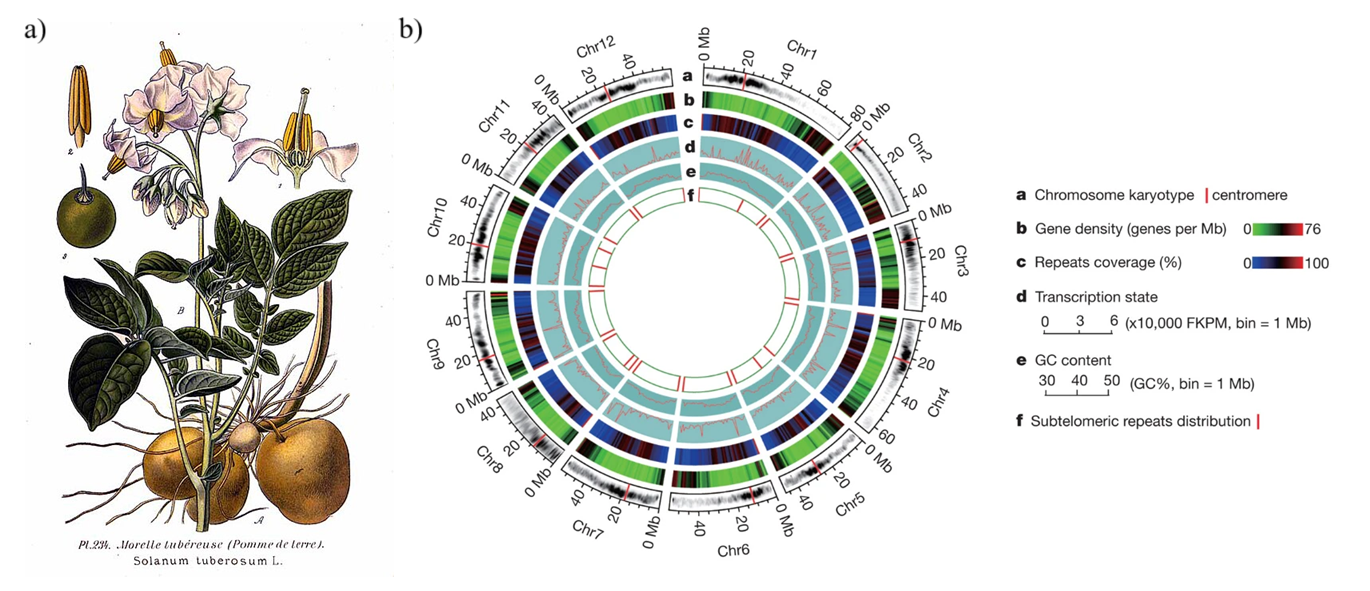
\includegraphics[width=1\textwidth]{potato.png}
	\caption{\justifying{\footnotesize \textit{\textbf{\textit{S. tuberosum} morphological and genetic characteristics.} \footnotesize{Morphology of \textit{S. tuberosum} (a) illustrated by Amédée Masclef  \parencite{masclefAtlasPlantesFrance1891}, and ideograms (b) of the 12 pseudo- chromosomes \parencite{xuGenomeSequenceAnalysis2011} that compose the assembly we used as reference.}}}}
	\label{fig:potato}
\end{figure}

The potato genome consists of 12 chromosomes (Figure \ref{fig:potato}, b) with an haploid length of approximately 840 Mb, but the majority of potato cultivars are autotetraploid (2n = 4x = 48) and, additionally, suffer from acute inbreeding depression \parencite{xuGenomeSequenceAnalysis2011}, due to their pedigree containing the same cultivars more than once in their ancestry \parencite{sunChromosomescaleHaplotyperesolvedGenome2022}. In fact, a recent study on the cultivar Otava showed that more or less 50\% of its genome is identical by descent (IBD), which results in 1.9 diverse allelic copies per gene \parencite{kuiSolanumTuberosumPotato2022}: the maximal allelic diversity in the potatoes is 4, so a value as low as 1.9 confirms a reduced genetic diversity shared by many of the modern cultivars of potatoes. This problem is exacerbated by the production method used almost globally: potatoes are usually propagated through the tubers - whole, a portion \parencite{reddyReviewPotatoSolanum2018} or through the buds \parencite{wangStudyCultivationSeedlings2022} - which means that individuals are cloned and not generated by crossing. This reduces costs and ensures that optimal characteristics (larger production per plant, less bitterness, bigger tubers...) are selected \parencite{wangStudyCultivationSeedlings2022}. Artificial selection can cause enrichment of specific genes: for example, in another study again on cultivar "Otava", it was shown that there was a positive correlation between selection-induced reduction of allelic diversity and enrichment of genes involved in photosynthesis, chlorophyll binding and translation \parencite{sunChromosomescaleHaplotyperesolvedGenome2022}. The inbreeding depression of \textit{S. tuberosum} raises concern because it decreases both breeding success \parencite{sunChromosomescaleHaplotyperesolvedGenome2022} and, more importantly, genetic diversity, which is essential for developing resistance to pathogens. Resistance to diseases is extremely important for crop plants: an example of this can be found in history, when in the 1840s blight disease attacked potatoes crops and caused the infamous Irish Potato Famine \parencite{wangStudyCultivationSeedlings2022}, which ultimately was the starting point of modern plant pathology.

\subsection{Sampling}
The samples used in this study can be divided in two categories: the modern landraces whose true origin was investigated as the research question, and the wild/ancient species used as group controls to answer it. The study involved a total of 12 local landraces of \textit{S. tuberosum}, 2 commercial cultivars (Desiree and Kennebec) of the same species, 4 wild and 4 ancient cultivated species of the same genus whose data was collected from the NCBI database (Table \ref{tab:solanum}). Classification of cultivated potatoes can change depending on their identification as species (as stated by the International Code of Botanical Nomenclature) or as as cultivar groups (International Code of Nomenclature of Cultivated Plants; \cite{huamanReclassificationLandracePopulations2002}): in this analysis, we followed ICBN classification as separated species \parencite{turlandInternationalCodeNomenclature2018}. 

\begin{table}[h!]
	\centering
	\caption{\textbf{List of commercial cultivars and local landraces of \textit{S. tuberosum} and wild/ancient species of genus \textit{Solanum}.}}
	\label{tab:solanum}
	\resizebox{\textwidth}{!}{
		\begin{tabular}{lll}
			\toprule
			\multicolumn{3}{c}{\textbf{ \textit{S. tuberosum} landraces}} \\
			\midrule
			\textbf{Species} & \textbf{Cultivar} & \textbf{Origin} \\
			\midrule
			\textit{S. tuberosum} & Kennebec & Commercial, USA \\
			\textit{S. tuberosum}  & Desiree & Commercial, Netherlands \\
			\textit{S. tuberosum}  & Bossico (BG) 1 & Teglio (SO) \\
			\textit{S. tuberosum} & Bossico (BG) 2 & Bossico (BG) \\
			\textit{S. tuberosum}  & Starleggia Rossa & Campodolcino (SO) \\
			\textit{S. tuberosum}  & Starleggia Bianca & Campodolcino (SO) \\
			\textit{S. tuberosum}  & Quarantina Genovese Bianca & Oltrepò (PV) \\
			\textit{S. tuberosum}  & Quarantina Genovese & Genova (GE) \\
			\textit{S. tuberosum}  & Comasca Biancona & Como (CO) \\
			\textit{S. tuberosum}  & Rossa & ``La Campagnola'' farm, Gordona (SO) \\
			\textit{S. tuberosum}  & Bianca & ``La Campagnola'' farm, Gordona (SO) \\
			\textit{S. tuberosum}  & Rossa Oltrepò, Romagnese & Ca' Novelli nel Romagnese (PV) \\
			\textit{S. tuberosum}  & Rossa Oltrepò di Pietragavina & Pietragravina (PV) \\
			\textit{S. tuberosum}  & Schilpario & Botanical garden of Bergamo (BG) \\
			\midrule
			\multicolumn{3}{c}{\textbf{Ancient cultivated species of genus \textit{Solanum}}} \\
			\midrule
			\textbf{Species} & \textbf{Accession Number} & \textbf{Origin} \\
			\midrule
			\textit{S. chaucha} & SRR10248511 & Andes \\
			\textit{S. phureja} & SRR10244439 & Bolivia, Peru, Venezuela, Colombia, Ecuador \\
			\textit{S. stenotomum} & SRR10244438 & Peru \\
			\textit{S. tuberosum} subsp. \textit{andigenum} & SRR10248514 & Andes \\
			\midrule
			\multicolumn{3}{c}{\textbf{Wild species of genus \textit{Solanum}}} \\
			\midrule
			\textbf{Species} & \textbf{Accession Number} & \textbf{Origin} \\
			\midrule
			\textit{S. microdontum} & SRR24976252 & Bolivia, Argentina \\
			\textit{S. vernei} & SRR24976381 & Bolivia, Argentina \\
			\textit{S. brevicaule} & SRR24976310 & Bolivia, Peru \\
			\textit{S. chacoense} & SRR24976359 & Bolivia, Peru, Argentina, Paraguay, Uruguay, Brazil \\
			\bottomrule
		\end{tabular}
	}
	\caption*{\footnotesize{\textit{List of commercial cultivars and local landraces of \textit{S. tuberosum} and wild/ancient species of genus \textit{Solanum}. The accession number associated with the wild/ancient species refers to specific runs on NCBI’s SRA database.}}}
\end{table}

The choice of which wild/ancient species to use in this analysis was influenced by: (i) other studies addressing being cultivated and evolutionary close to \textit{S. tuberosum} (i.e. \textit{S. phureja}, \cite{xuGenomeSequenceAnalysis2011}; \textit{S. stenotomum}, \cite{wangStudyCultivationSeedlings2022}; \textit{S. chauca}, \cite{huamanReclassificationLandracePopulations2002}), (ii) being wild (i.e. \textit{S. microdontum}, \cite{huamanReclassificationLandracePopulations2002}; \textit{S. vernei}, \cite{spoonerSystematicsDiversityGenetics2014}), prioritizing those (i.e. \textit{S. brevicaule} and \textit{S. chacoense}; \cite{huamanReclassificationLandracePopulations2002}) currently present in the wild were domestication started (Bolivia and Peru; \cite{dejongImpactPotatoSociety2016}), (iii) reads quality and sequences availability. Instead, data for landraces was obtained from living plants: seeds were provided by the seed bank of University of Pavia, after collection from its research institutes, public institutions and farms in the area. Samples were then grown at the University of Milan, and, after germination, their leaves were collected and stored at -80°C in the first half of 2024.

\subsection{Wet lab protocol}
DNA extraction was carried out in University of Milan following the same CTAB protocol employed for \textit{C. thyrsoides}, and then purified using Genomic DNA Clean \& Concentrator-10 kit by Zymo Research. Library preparation for GBS data was also performed in the same manner as described in the previous sections, using again restriction enzyme ApeKI to fragment the DNA, with a 2 hours incubation time at 75°C. As we previously mentioned, this was the classic protocol for digestion that was first employed in the laboratory to digest samples of \textit{S. lycopersicum} and that was modified to better fit \textit{C. thyrsoides} challenging digestion. \textit{S. tuberosum}, being part of the same genus as \textit{S. tlycopersicum}, did not need adjustments on incubation time. Ligation, Pooling and PCR amplification protocols were the same as described for \textit{C. thyrsoides}, minus the size-selection step which was skipped since it was not necessary for these samples. The 14 landraces' DNA libraries were sent to GENEWIZ from Azenta Life Sciences (Leipzig, Germany) for standard Illumina TruSeq combinatorial-dual DNA sequencing in the second half of 2024.

\subsection{Dry lab analyses}
Pre-processing of the data was performed by PhD Paleni Chiara for BSc graduate Giulia Ballarotti's thesis \parencite{ballarottiSolanumTuberosumNel2025} prior to our analysis, so the sequences' files were already de-multiplexed, trimmed and filtered at the beginning of this study. Nevertheless, the softwares and parameters used widely overlapped, with the only exception that cleaning was performed using software \texttt{fastq-mcf} (v1.05) with trimming of base-pairs based on the quality Phred score threshold of 30 ($-q \ 30$), minimum length after trimming of 50 bp ($-l \ 50$), disabling skew filtering ($-k \ 0$) and adding a window size set to 2 to further remove low quality bases ($-w \ 2$). The full list of commands used for these and the next steps can be found in the supporting file \texttt{Final\_report\_potatoes\_cultivars.html}, freely available in the \texttt{Github} repository associated with this thesis \texttt{flavialeotta\ master-thesis}.

\subsubsection{Variant calling with a reference genome}
The advantage of working with crops plants is that, more often than not, a reference genome is available: this is the case of \textit{S. tuberosum} for which an official reference genome can be found on NCBI, and which we used for variant calling. The chromosome-level genome assembly we used is file "Solanum\_tuberosum.SolTub\_3.0.dna.toplevel.fa" corresponding to GenBank assembly GCA\_000226075.1 (available in release-62 of Ensemble genomes at https://ftp.ensemblgenomes.ebi.ac.uk/pub/plants/release-62/fasta/solanum\_tuberosum/dna/), which, in turn, was built on scaffold-level assembly NCBI RefSeq GCF\_000226075.1 submitted by Beijing Genomics Institute in Shenzhen, China \parencite{xuGenomeSequenceAnalysis2011}. This sequence accession number corresponds to an homozygous diploid cultivar \textit{S. tuberosum} group Phureja strain DM1-3 516 R44\footnote{DM1-3 516 R44 is the result of chromosome doubling of a monoploid (1n = 1x = 12) derived by a heterozygous diploid (2n = 2x = 24) \textit{S. tuberosum} group Phureja clone (PI 225669; \cite{xuGenomeSequenceAnalysis2011}).}. Sequences files associated with other wild species of genus \textit{Solanum} were downloaded through their accession number (Tab. \ref{tab:solanum}) using SRA Toolkit. All samples, both landraces and wild/ancient species, were mapped on the same reference genome using a custom script \texttt{map\_bwa.sh} which recursively maps (\texttt{bwa mem}, v0.7.19; \cite{liAligningSequenceReads2013}) on the reference genome and then converts the generated \texttt{.bam} files in a \texttt{.sam} file, using \texttt{samtools} (v1.21; \cite{danecekTwelveYearsSAMtools2021}). After doing this for every sample, all \texttt{.sam} files are sorted  (\texttt{samtools}) and merged (\texttt{bamaddrg}\footnote{Version 9baba65f88228e55639689a3cea38dd150e6284f \parencite{garrisonEkgBamaddrg2025}.}). The resulting \texttt{.bam} file is indexed (\texttt{samtools}) and then converted in a \texttt{.bed} file using \texttt{bedtools} (v2.29.0; \cite{garrisonEkgBamaddrg2025}). To speed up the analysis, we employed \texttt{MultiThreadFreeBayes}(v0.1\footnote{From GenoToolBox \parencite{bombarelyGenoToolBoxBoxGenomics2020}. It depends on \texttt{freebayes} (v1.38; \cite{garrisonHaplotypebasedVariantDetection2012})}), a script that supports multithreading of the golden standard \texttt{freebayes}, and performed the final step of variant calling: we only kept SNPs called with a minimum base quality of 30 ($-m = 30$), minimum mapping quality of 30 ($-q = 30$), and lower and upper coverage limits of 10 and 1000 ($\text{--limit-coverage} = 100$, $\text{--min-coverage} = 10$). After some intermediate steps to prepare the input file, we filtered the \texttt{.vcf} using \texttt{vcftools} with the same parameters used for \textit{C. thyrsoides}, with the exception of minor allele frequency threshold being set to 0.023 (calculated using formula \ref{formula:maf} and $n = 22$ biallelic samples) and maximum missing data to 5\% ($\text{--max-missing} \ 0.95$). The latter is a slightly more stringent threshold than what was used with \textit{C. thyrsoides} ($\text{--max-missing} \ 0.90$) since working with a reference genome allows us to be stricter with the quality of called SNPs, without losing information. Additionally, for each sample, we obtained \texttt{.bed} files with the intervals of the regions covered by samples' reads, along with their coverage (\texttt{bedtools}). These files are intersected to find the shared sites between all of the samples and we stored the information found in a text file. Lastly, the generation of the phylogenetic tree followed the same workflow as \textit{C. thyrsoides}: the evolutionary model chosen by program \texttt{ModelFinder} was TVM+F+ASC+G4.

\newpage
\section{\textit{Anacamptis} spp.}
Orchids are one of the largest family, which accounts for about a tenth of flowering plants \parencite{yinPlantConservationAge2024}. A large percentage of them are regarded as threatened or endangered \parencite{yinPlantConservationAge2024}.

\subsubsection{\textit{Anacamptis pyramidalis}}
\subsubsection{\textit{Anacamptis berica}}

\subsection{Wet lab protocol}
Do I really need to go into details? I would just say that they used two restriction enzymes, but since the data was cleaned and filtered before being given to me, I did not have to apply this knowledge of any step.

\subsection{Dry lab analyses}
The data for \textit{Anacamptis pyramidalis} and \textit{Anacamptis berica} was provided by University of Vienna already filtered and cleaned, so the same pipeline was applied starting from the variant calling step (\autoref{variant-calling}). Hyperparameters optimization for \texttt{STACKS}: \texttt{denovo\_map.pl} pipeline wasn't needed, as the chosen parameters were previously assessed by PhD candidate Scamorcin Lisa, and selected as $m = 3, \ M = 4, \ n = 4$. All of the subsequent analyses were carried in the same way as previously discussed.



\clearpage
\chapter{Results}

\section{\textit{Campanula thyrsoides}}
\vspace{-1em}
Unfortunately, the whole CAN population consisting in the majority of the outgroup of \textit{Campanula thyrsoides} subsp. \textit{thyrsoides} had to be excluded from the library preparation step because the samples showed little to no DNA material after digestion (\autoref{Materials and Methods}). Nevertheless, the individuals from population CTT could still be used as the outgroup to which confront the individuals of the subspecies \textit{carniolica}. From the original 153, only 106 individuals across 10 populations were used to build the library and thus were sequenced, with a mean of 10.6 individuals per population (excluding CAN). Of this dataset, another 3 samples were excluded during the dry lab analysis, precisely on the filtering step: ALP11, LPASS5 and LPASS6 were excluded because they comprised of less than 1 million pairs of reads (ALP11 had 576927 pairs, LPASS5 934941 and LPASS6 only 25314). Such low value of reads would have reduced the mean coverage of their populations (ALP and LPASS), and moreover, considering the filters applied to the SNPs later in the analysis, would have led to the exclusion of informative loci because of an higher percentage of missingness across samples.

\subsection{Pipeline refinement}
\subsubsection{Improvement of trimming}
\vspace{-1em}
Using \texttt{fastp} instead of \texttt{fastq-mcf} resulted in a substantial improvement in performance. The wall-clock execution time decreased from around 30 minutes to more or less 4.5 minutes, corresponding to a speedup of approximately 7x and a reduction in runtime of ~85\%. The user CPU time reported by \texttt{fastp} was higher (62 minutes vs. 40 minutes for \texttt{fastq-mcf}), indicating that \texttt{fastp} is more CPU-intensive, due to parallelized operations. However, because this additional computation is efficiently distributed across cores, the overall elapsed time is cut to half (from slightly more than 1 minute to just 29 seconds), suggesting less overhead in I/O operations. The quality of the cleaning remained the same if not better with \texttt{fastp}, since this software is able to efficiently cut off the majority of the poly-G tails (Figure \ref{fig:fastp}) by sacrificing slightly the average length of reverse reads (from 83bp to 80bp) but still retaining the same amount of reads (i.e. 2.6 millions for ALP1) as \texttt{fastq-mcf} does. Length of reads might seem short, but it is common in GBS protocols \parencite{elshireRobustSimpleGenotypingbySequencing2011}.

\begin{figure}[h!]
	\centering
	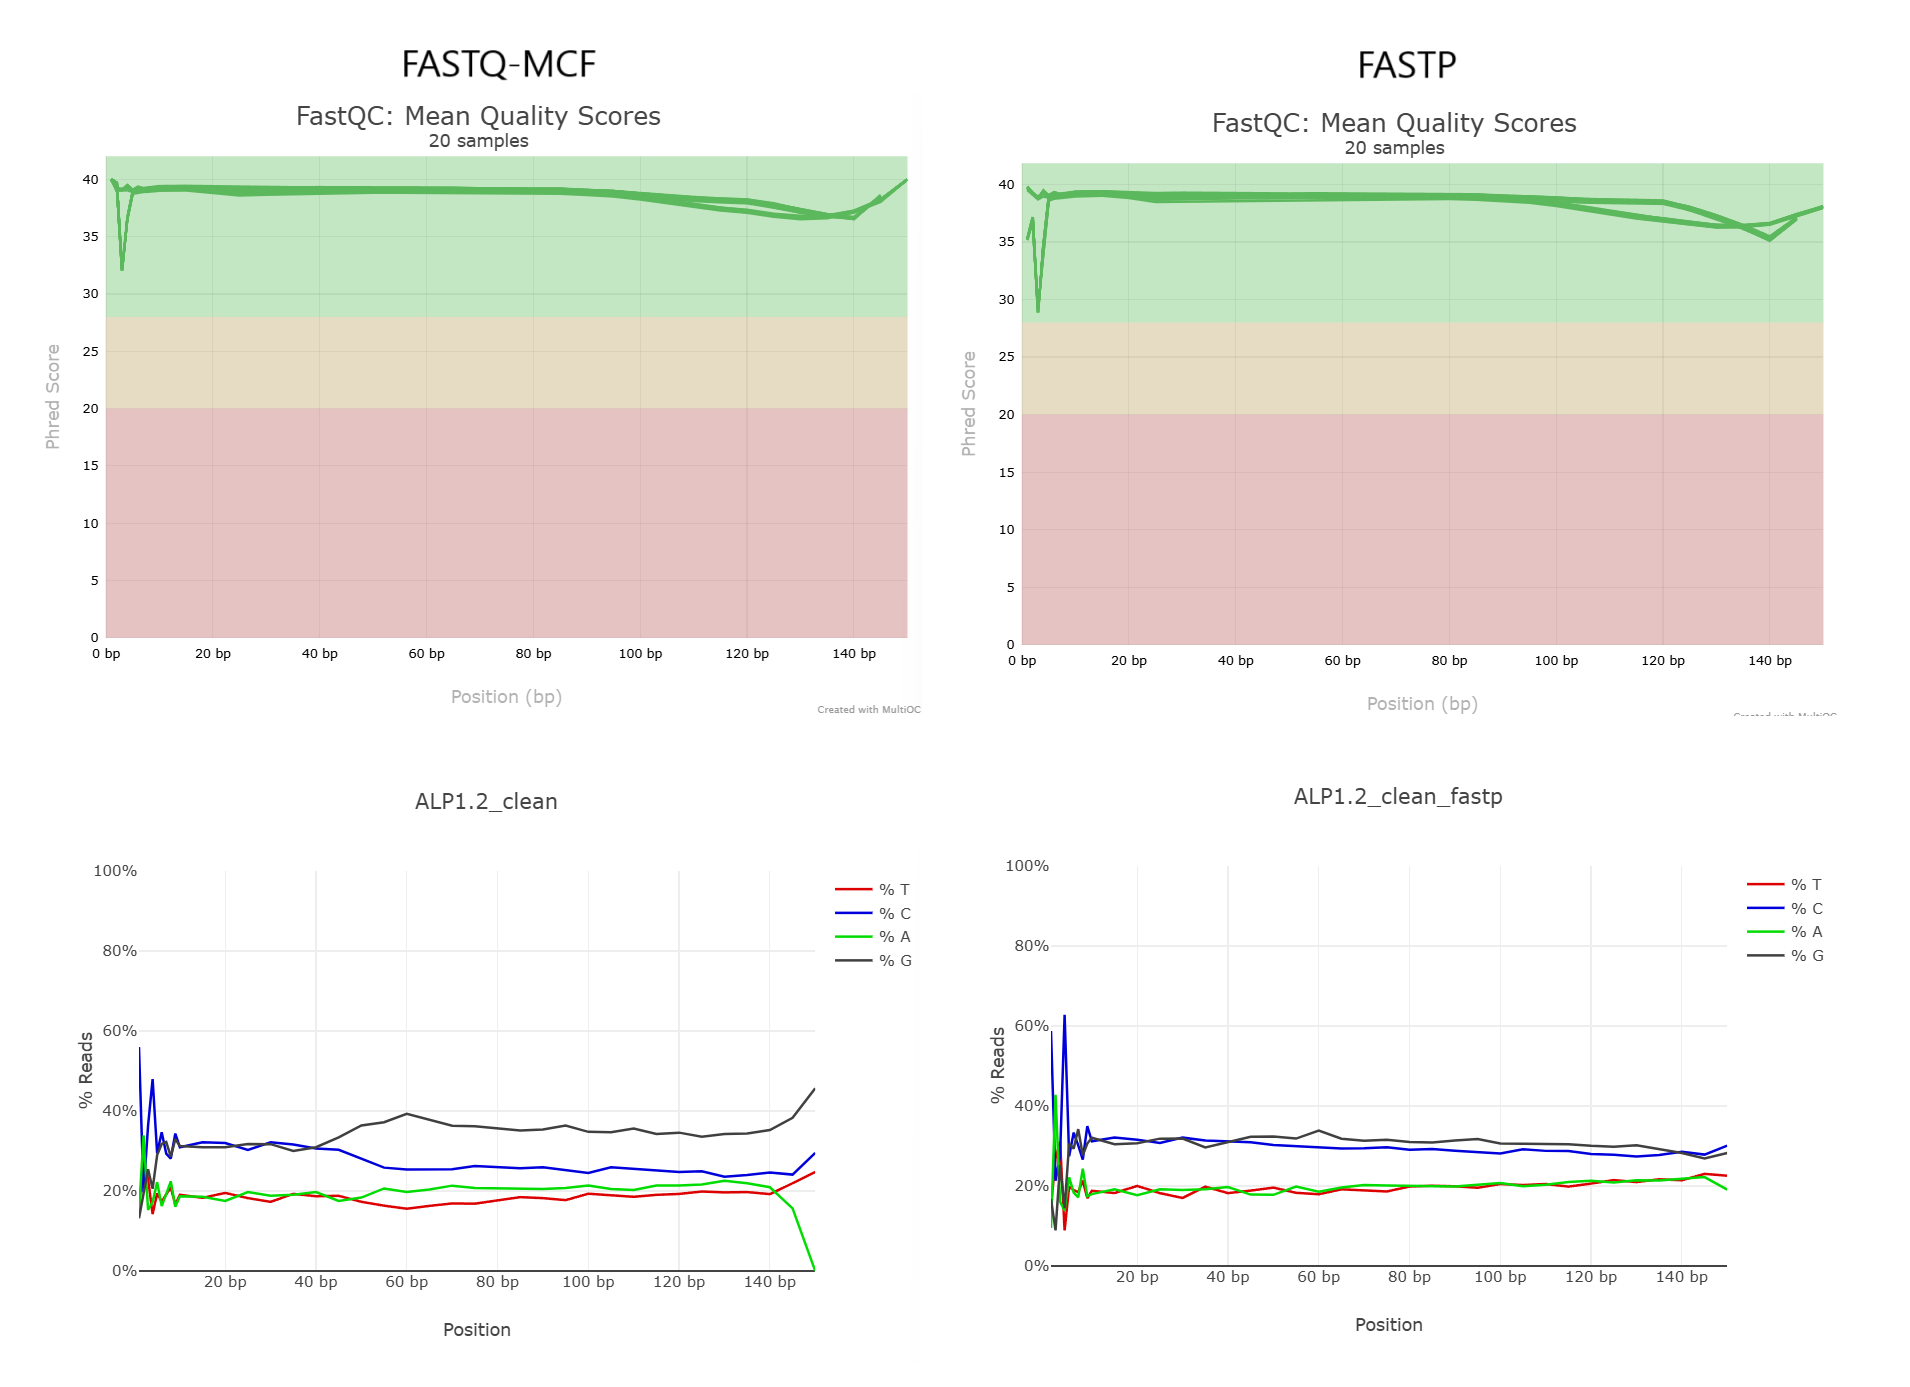
\includegraphics[width=0.8\linewidth]{fastqmcf_fastp_comparison.png}
	\caption{\justifying{\footnotesize \textit{\textbf{Comparison between cleaning tools} \footnotesize{When using the correct parameters, \texttt{fastp} maintains a good overall reads' quality (top) and trims poly-G tails better (bottom plot). Plots built using software \texttt{FastQC} (v0.11.5; \cite{andrewsFastQCQualityControl2010}) and \texttt{multiqc} (v1.27.1; \cite{ewelsMultiQCSummarizeAnalysis2016}).}}}}
	\label{fig:fastp}
\end{figure}

\subsubsection{Hyperparameters' tuning outcome}
\vspace{-1em}
When exploring the percentage of lost reads during the process of variant calling, we've noticed that the majority of the information is lost at the last step, meaning the \texttt{Stacks:} \texttt{denovo\_map.pl} pipeline implementation (Figure \ref{fig:lost reads}). This highlights the need to accurately tune this pipeline, as to maximize the amount and the quality of information we are able to gather from sequencing data.

\begin{figure}[h!]
	\centering
	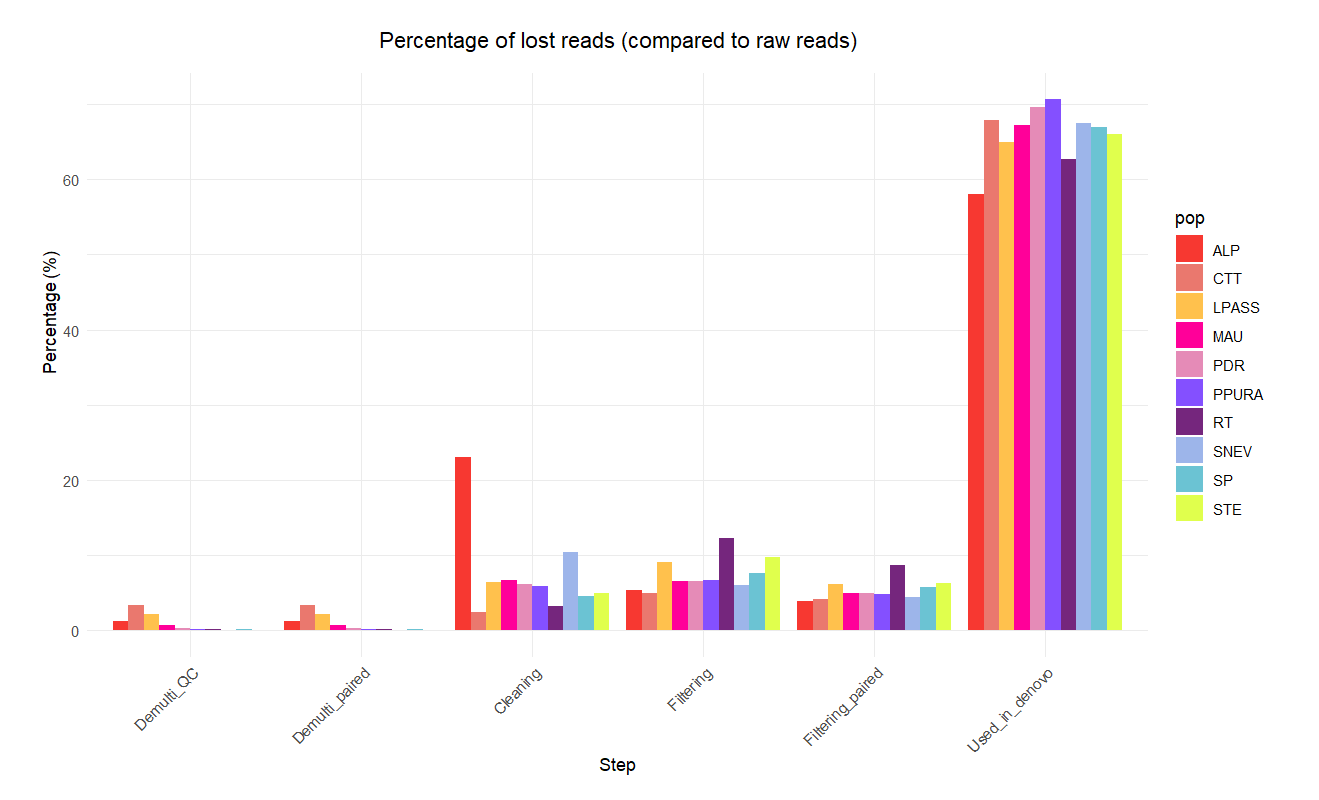
\includegraphics[width=0.9\linewidth]{Barplot_lost_reads.png}
	\caption{\justifying{\footnotesize \textit{\textbf{Lost reads at each step} \footnotesize{Barplot showing the percentage of discarded reads (in comparison to the amount of raw reads) at each step, from pre-processing to variant calling, grouped by population.}}}}
	\label{fig:lost reads}
\end{figure}
We tested a total of 46 combinations of parameters for \texttt{Stacks:} \texttt{denovo\_map.pl} on a subset of 9 samples from population ALP, and whose performance is reported in Table \ref{tab:denovo_parameters} in the Additional Materials chapter. The best combination out of them was $m = 4$, $M = 1$ and $n = 1$: interestingly enough, by using the score function \ref{eq:score} to assess their performance, the only combinations that passed the required conditions (an average coverage of 10x and at least 2400 called loci) always had $m = [4,5]$ (Fig. \ref{fig:denovo}), suggesting that this might be the most important parameter to tune.

\begin{figure}[h!]
	\centering
	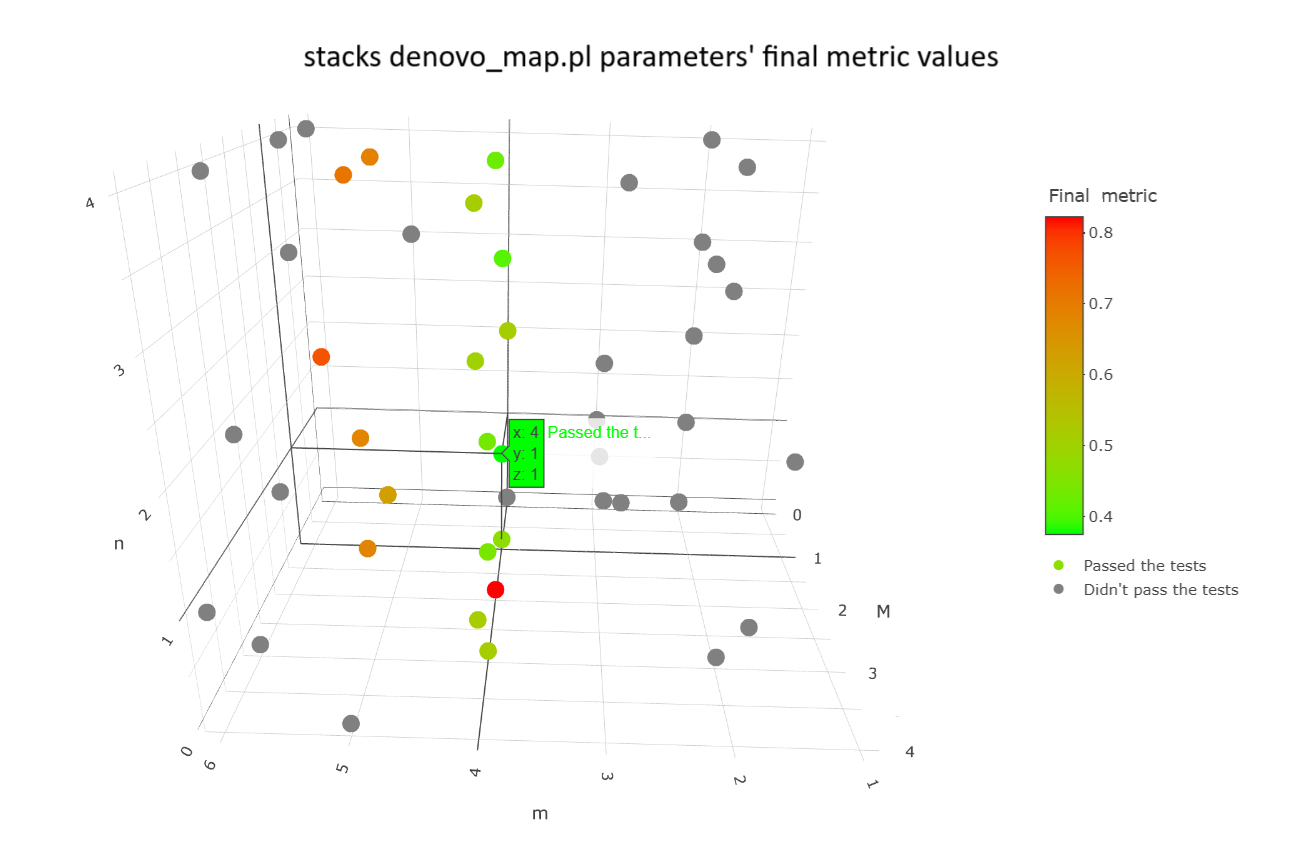
\includegraphics[width=0.7\linewidth]{denovo_map_metrics.png}
	\caption{\justifying{\footnotesize \textit{\textbf{Score function values plotted for 45 combinations} \footnotesize{3D plot of the combinations of \texttt{Stacks}: \texttt{denovo\_map.pl}'s parameters tested, colored by score function (Equation \ref{eq:score}) results. The best combination (m = 4, M = 1, n = 1) is highlighted.}}}}
	\label{fig:denovo}
\end{figure}

To assess how changing the parameters influenced our results, we built regression models to find the mathematical relationship between 'm', 'M' and 'n', and the metrics we were interested in. We used R package \texttt{stats} to build the following models:
\vspace{-1.5em}
\begin{itemize}\setlength\itemsep{-0.2em}
	\item For the \textbf{mean coverage ($\mu_{cov}$)} we found a significant linear relationship (p-value $< 2.2\text{e-}16$) that is able to well explain the variability of our data (for a 10-fold cross validation repeated 30 times, $R^2 = 0.9980 \pm 0.0017$):
	\begin{equation}
		\mu_{cov} = -0.93293+2.88617\cdot m+0.07947\cdot M
	\end{equation}
	with 'm' being very significative (p-value $< 2.2\text{e-}16$) and 'M' slightly less (p-value $= 0.00244$). The fact that 'n' is not significative at all is to be expected, since the coverage of samples is computed after the first step of the pipeline (\texttt{ustacks}) which uses only parameters 'm' and 'M'.
	\item The \textbf{standard deviation of the coverage $\sigma_{cov}$}, instead, depends only on the value of 'm', with p-value $< 2.2\text{e-}16$ and 10-fold cross validation (30 repetitions) $R^2 = 0.9149 \pm 0.1881$:
	\begin{equation}
		\sigma_{cov} = 0.32135+0.25138\cdot m
	\end{equation}
	The goal of parameter tuning is to find the correct parameters that result in an high coverage with a small standard deviation: unfortunately, increasing 'm' leads to higher values of both, so $m < 4 \vee m > 5$ both do not pass the requirement of minimum coverage.
	\item To summarize both quantities, we tried to build a model that describes the \textbf{coefficient of variation (CV)} as the ratio between standard deviation and mean of the coverage (p-value$=5.251\text{e-}08$, 10-fold cross validation $R^2 = 0.8205 \pm 0.2667$):
	\begin{equation}
		CV = 0.189629 - 0.044843 \cdot log(m)
	\end{equation}
	We found again that only the value of 'm' was significative, but the model was less robust than the previous ones so we decided to consider the two quantities separately;
	\item Building a model for the number of called SNPs and unique loci proved to be more complicated. When building a linear model using all parameters, we get a less robust model ($R^2 \sim 0.70$) than what was explored before with mean and standard deviation of coverage. Using only 'm' and increasing the complexity to the fourth polynomial would have raised the training $R^2$ up to almost 0.99, but it would have drastically reduced the test $R^2$ to levels as low as $0.59 \pm 0.33$ for SNPs and $0.52 \pm 0.34$ for unique loci, a textbook case of overfitting. The best model for the number of \textbf{SNPs} included all the parameters and was built to predict SNPs on a logarithmic scale. With p-value $= 6.061\text{e-}06$ and 10-fold cross validation (30 repetitions) $R^2 = 0.7603 \pm 0.2805$, the model is the following:
	\begin{equation}
		log(SNPs) = 9.08393 -0.3486 \cdot m + 0.19492 \cdot M + 0.19022 \cdot n
	\end{equation}
	\item Similarly as before, for the number of \textbf{unique loci} we obtained:
	\begin{equation}
		log(unique \ loci) = 8.98525 -0.36520 \cdot m + 0.13172 \cdot M + 0.13584 \cdot n
	\end{equation}
	with p-value $= 1.157\text{e-}05$ and 10-fold cross validation (30 repetitions) $R^2 = 0.7747 \pm 0.2645$.
\end{itemize}
\vspace{-1.5em}
We used these regression models to test their ability to predict how the metrics could change in any of the combinations we had not tried up to that moment. We used library \texttt{scikit} on Python which run these regression models on the whole search space discussed in the Materials and Methods chapters: the optimal solution found was $m = 4$, $M = 0$ and $n = 4$. We tried running these parameters since they had not been explored during training, and we show the comparison between  observed and predicted results in Table \ref{tab:pred_vs_obs}.

\begin{table}[ht]
	\centering
	\caption{\textbf{Observed and Predicted metrics for combination $m = 4$, $M = 0$ and $n = 4$.}}
	\label{tab:pred_vs_obs}
	\begin{tabularx}{\textwidth}{XXX}
		\hline
		\textbf{Metric} & \textbf{Observed} & \textbf{Predicted} \\
		\hline
		$\mu_{cov}$    & 10.8323 & 10.5964 \\
		$\sigma_{cov}$ & 1.42895 & 1.3248  \\
		CV             & 0.1319  & 0.1250  \\
		SNPs           & 5264    & 4618    \\
		Unique loci    & 3274    & 4055    \\
		\hline
	\end{tabularx}
	\caption*{\footnotesize{\textit{Comparison between the observed results when running \texttt{denovo\_map.pl} pipeline, and the ones predicted by the regression models.}}}
\end{table}
\vspace{-1em}
These values show that the models underestimate all results: undervaluing the mean coverage, SNPs and unique loci would have led this solution to be considered not ideal (big values of unique loci are a reward in the score function), but it also underestimated the penalty values, namely the standard deviation of the coverage (thus CV too) and the ratio of SNPs per locus. Underestimating the penalties, which are numerically more than the rewards and can easily outweigh them\footnote{In function \ref{eq:score} these quantities are all normalised, carrying the same weight $\in [0,1]$.} in the model, led to an overall better score for this combination of parameters, which in reality showed a worse combination than combination $m = 4, M = 1, n = 1$. We concluded that those models that include 'M' or 'n' (i.e. the ones for SNPs and unique loci) do not greatly improve the results from those that only included 'm', so while the optimal 'm' is easily identified, the ideal 'M' and 'n' might be more difficult to find. These regression models are of course specific to the subset we built them on and cannot be used in general to predict the parameters in other contexts: we suggest to test datasets case by case, prioritizing the choice of 'm' over both 'M' and 'n'.

\subsubsection{\textit{De novo} assembly}
\vspace{-1em}
In the pipeline \texttt{Stacks}: \texttt{denovo\_map.pl}, the first step \texttt{ustacks} builds loci \textit{de novo} in each sample: each individual has its own coverage, computed across its own loci. We obtained a mean coverage of $16.31 \pm 4.37$ ($median = 15.71$) over 103 samples across 10 populations: only one sample had less than 10x coverage (ALP6, having 8.94x) and only one sample had an outlier value (STE8, coverage = 41.09x; Figure \ref{fig:coverage}).

\begin{figure}[h!]
	\centering
	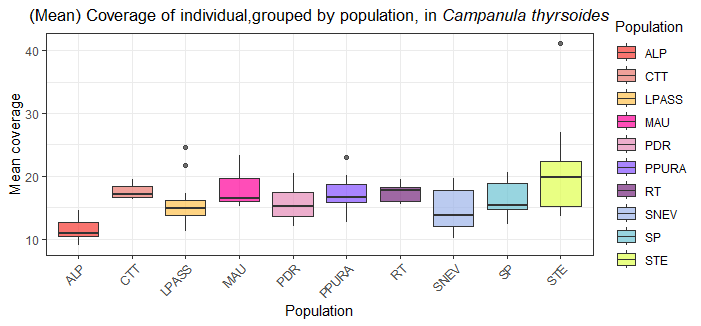
\includegraphics[width=0.8\linewidth]{meancov_populations.png}
	\caption{\justifying{\footnotesize \textit{\textbf{Coverage across samples} \footnotesize{Boxplots of coverage of samples of \textit{C. thyrsoides}, grouped by population.}}}}
	\label{fig:coverage}
\end{figure}

After building the loci catalogue using \texttt{cstacks} and mapping each samples through \texttt{sstacks} as described in the Materials and Methods section, the second to last step is running program \texttt{gstacks}. It was able to build consensus sequences for 4,313,775 loci by assembling paired-end contigs for 99.9\%\footnote{The remaining 0.1\% of reads didn't successfully form a paired-end contig.} of them: of these, 97.7\% overlapped (average overlapping region was 30.9 bp long). The average length of contigs was 103.1 bp. Then, out of ~398 million paired-end reads, aligned 99.9\% on the assembled contigs and performed SNP calling. Since we are in a \textit{de novo} setting SNPs can not be exactly located on chromosomes, so their position was defined over the aforementioned assembled contigs. The estimated mean insert size was 110.1 bp ($\pm$ 49.3 bp). In total, 4,307,333 loci were genotyped with an effective mean coverage of 21.1x $\pm$ 7.2x (ranging from 10.9x to 61.6x). These results prove the high quality of the \textit{de novo} assembly, with a large fraction of the assembled loci having sufficient read coverage and being successfully genotyped. This ensures that the downstream population genomic analyses are going to be as reliable as possible.

\subsubsection{Filtering}
\vspace{-1em}
We tested two different software and methods to filter out non informative and low-coverage SNPs: \texttt{population} and \texttt{vcftools}. When filtering through the \texttt{denovo\_map.pl} pipeline itself, we used command:
\begin{lstlisting}
	1) populations -r 0.80 -R 0.80 --write-random-snp --min-mac 2
\end{lstlisting}
\vspace{-1.2em}
which kept 9556 out of a possible 126379 Sites. Instead, when using \texttt{vcftools} we run:
\begin{lstlisting}
	1) populations -r 0.80
	2) vcftools--max-missing 0.9 --minDP 5 --min-meanDP 5 --thin 1000 --maf 0.005 
	3) populations --write-random-snp
\end{lstlisting}
\vspace{-1.2em}
which kept 3,896 out of a possible 126,379 Sites. To keep the comparison between the two methods simple, in the code above we only reported the filtering parameters and not those for input and generation of output files. While flags $-R \ 0.80$ in \texttt{populations} and $\text{--}max\text{-}missing \ 0.9$ in \texttt{vcftools} equally define a minimum percentage of individuals to process a locus, the rest have a slightly different effect, although they try to apply the same filtering principle. When trying to filter out rare SNPs, we applied $\text{--}min\text{--}mac 2$ in \texttt{populations} and $\text{--}maf 0.005$ in \texttt{vcftools}. The first is criterion sets a minimum minor allele count process a SNP (\textbf{absolute} value), while the second defines a threshold for minor allele frequencies (\textbf{relative} value). We've noticed that while filtering using \texttt{populations} retains more SNPs (9556 vs 3896), it also increases the amount of missing data (Fig. \ref{fig:filtering}, a), with the whole population of ALP having between 50 to 60\% of missing SNPs information.

\begin{figure}[h!]
	\centering
	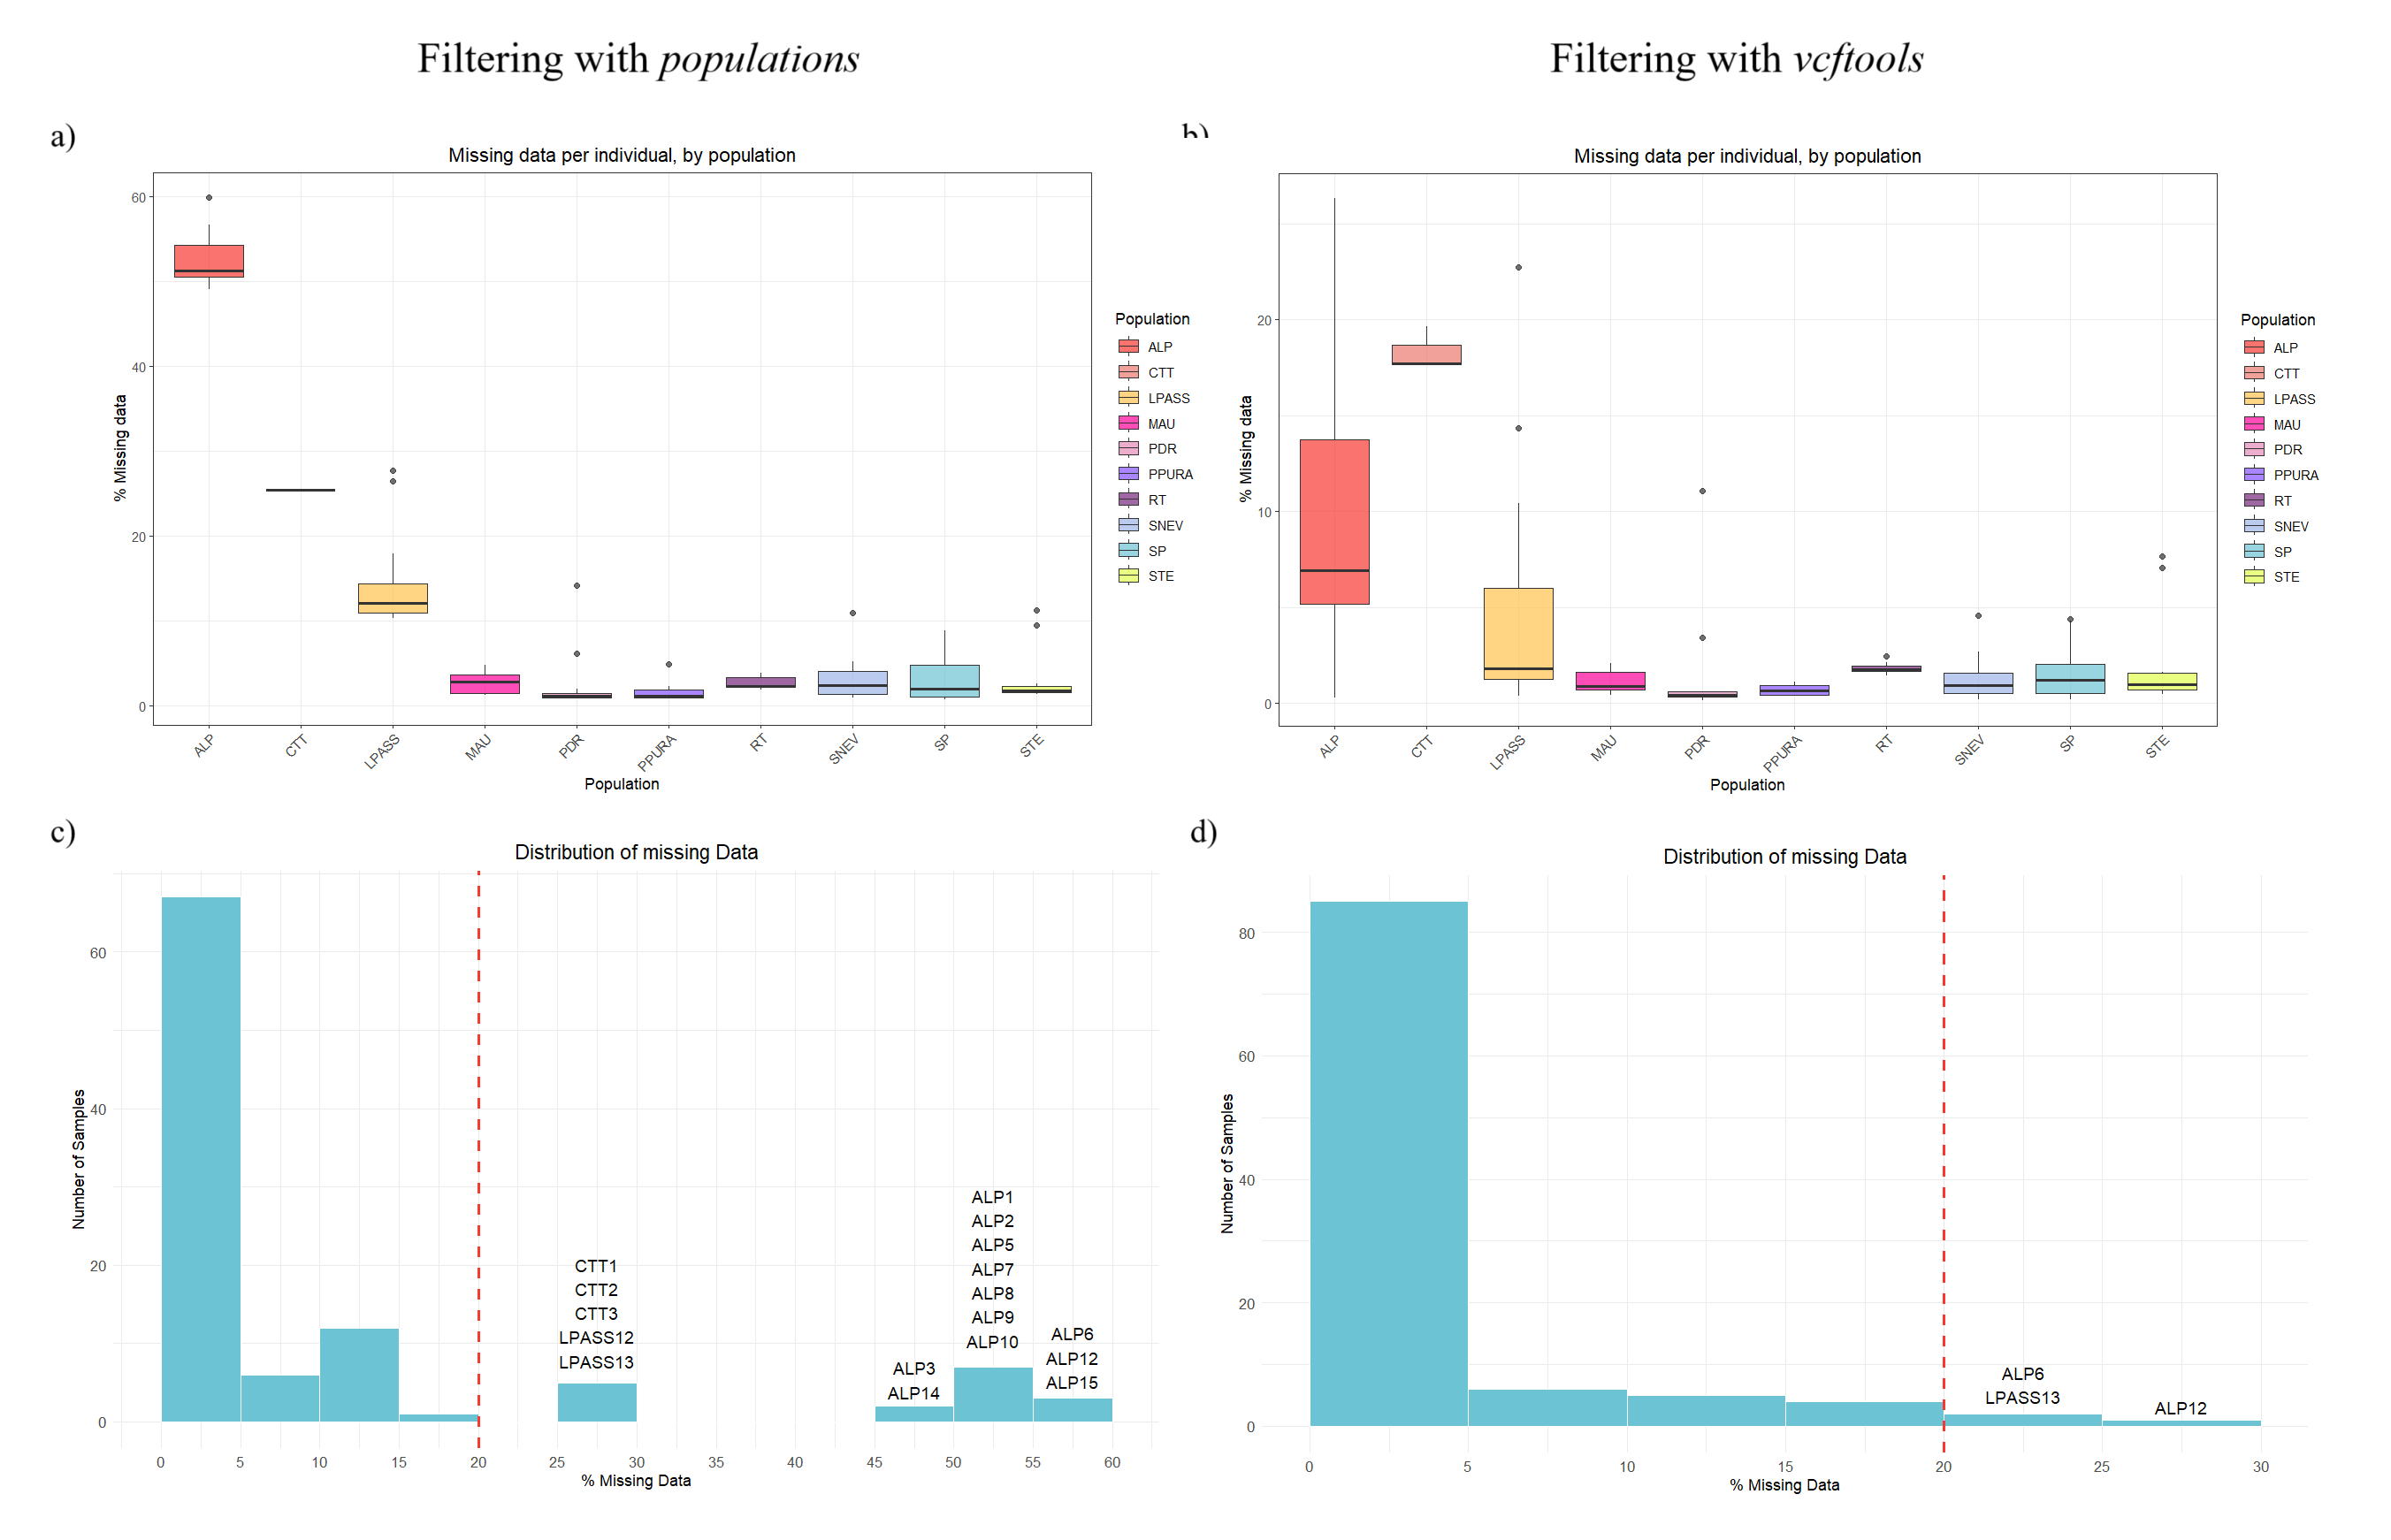
\includegraphics[width=0.9\linewidth]{filtering_methods.png}
	\caption{\justifying{\footnotesize \textit{\textbf{Comparison between filtering methods} \footnotesize{Boxplots (a, b) and barplots (c, d) of missing data in each individual. When filtering through \texttt{populations} (a, c), these plots are based on 9556 SNPs, when filtering through \texttt{vcftools} (b, d) it is based on 3896 SNPs.}}}}
	\label{fig:filtering}
\end{figure}

 This is not ideal, since the individuals from that population might cluster together just on the basis of missing the majority of the data, instead of real similarity between them. While populations of Alpago (ALP), Loiblpass (LPASS) and the outgroup \textit{thyrsoides} (CTT) are still missing more data than the others even when using \texttt{vcftools} (Fig. \ref{fig:filtering}, b), the distribution of the percentage of missing data drastically decreases. Not only that, but when setting a threshold of maximum 20\% of missing data to be considered in the next analysis, when filtering through \texttt{populations} 17 samples would not pass this condition  (Fig. \ref{fig:filtering}, c), while when using \texttt{vcftools}, only 3 samples would be excluded  (Fig. \ref{fig:filtering}, d). This is why we ultimately chose to filter SNPs using \texttt{vcftools}. 
 
\subsection{Dry lab analysis}
\subsubsection{Variant calling}
\vspace{-1em}
We filtered the file using \texttt{vcftools} and run software \texttt{populations} again to compute populations' statistics (Table \ref{tab:pop_stat}). Some loci in each population deviate from HWE: in literature they are often filtered out from the analysis, but, because the percentage is small (0\% to 5.1\%) and their presence is expected when there is overlapping of generations and very small population sizes \parencite{pearmanCommonlyUsedHardy2022}, we did not remove them from our dataset. The final array of SNPs comprehended 3896 polymorphic SNPs when including the outgroup CTT and 3558 when excluding it.

\begin{table}[ht]
	\centering
	\caption{\textbf{Populations' statistics}}
	\label{tab:pop_stat}
	\resizebox{\textwidth}{!}{%
		\begin{tabular}{lccccccc}
			\hline
			Population & $\pi$ & All sites & Variant & Polymorphic & Private alleles & Sites out HWE & \% out HWE \\
			\hline
			ALP   & 0.098848 & 3896 & 3896 & 1223 & 135 & 128 & 3.29\% \\
			CTT   & 0.076954 & 3211 & 3211 & 480  & 297 & 0   & 0.00\% \\
			LPASS & 0.103980 & 3896 & 3896 & 1206 & 183 & 106 & 2.72\% \\
			MAU   & 0.085217 & 3884 & 3884 & 859  & 49  & 91  & 2.34\% \\
			PDR   & 0.066905 & 3896 & 3896 & 750  & 107 & 127 & 3.26\% \\
			PPURA & 0.112200 & 3896 & 3896 & 1523 & 157 & 197 & 5.06\% \\
			RT    & 0.129100 & 3855 & 3855 & 1411 & 287 & 88  & 2.28\% \\
			SNEV  & 0.093674 & 3896 & 3896 & 1098 & 115 & 116 & 2.98\% \\
			SP    & 0.102140 & 3896 & 3896 & 1369 & 172 & 140 & 3.59\% \\
			STE   & 0.119470 & 3896 & 3896 & 1576 & 364 & 141 & 3.62\% \\
			\hline
		\end{tabular}%
	}
	\caption*{\footnotesize{\textit{All populations' statistics are calculated by \texttt{populations}. "$\pi$" is the average number of nucleotide differences per site; "All sites" is the total number of loci analyzed in that population;  "Variant" is the number of loci with at least one variant allele in the whole dataset; "Polymorphic" are loci variable within the population; "Sites out HWE" are variable sites that significantly deviate from Hardy-Weinberg equilibrium ($p<0.05$); "\% out HWE" is the percentage of sites out of HWE, calculated over variant loci.}}}
\end{table}

\subsubsection{Spatial separation}
The final set of 3896 polymorphic SNPs revealed a good separation of the populations: in Figure \ref{fig:PCA} we show plots of the first three principal components for datasets including (a, b, c) and excluding (d, e, f) the outgroup CTT (subspecies \textit{carniolica}). Almost all populations' clusters are well defined and separated: furthermore, in the top plots, CTT separates from the subspecies \textit{carniolica} along the third Principal Component (PC; 6.92\% of variance explained), which validates the choice of this population as the outgroup of the study. When excluding CTT, the first PC, which explains $12.55\%$ of the variance of the samples, captures a Longitude gradient from East to West, starting from the Slovenian-Austrian populations and ending with the population from Lombardia (Italy). The three populations from outside of Italy (LPASS, Austria, RT and STE, Slovenia) are better separated along PC3 when the outgroup is not included (Fig. \ref{fig:PCA}, e and f). All the populations of regions Veneto and Friuli (SP, MAU, PPURA, ALP) cluster together, with the exception of the population on the border of Italy and Slovenia (SNEV) which in the PCA plots is always located between the Austrian and Italian populations.

\begin{figure}[h!]
	\centering
	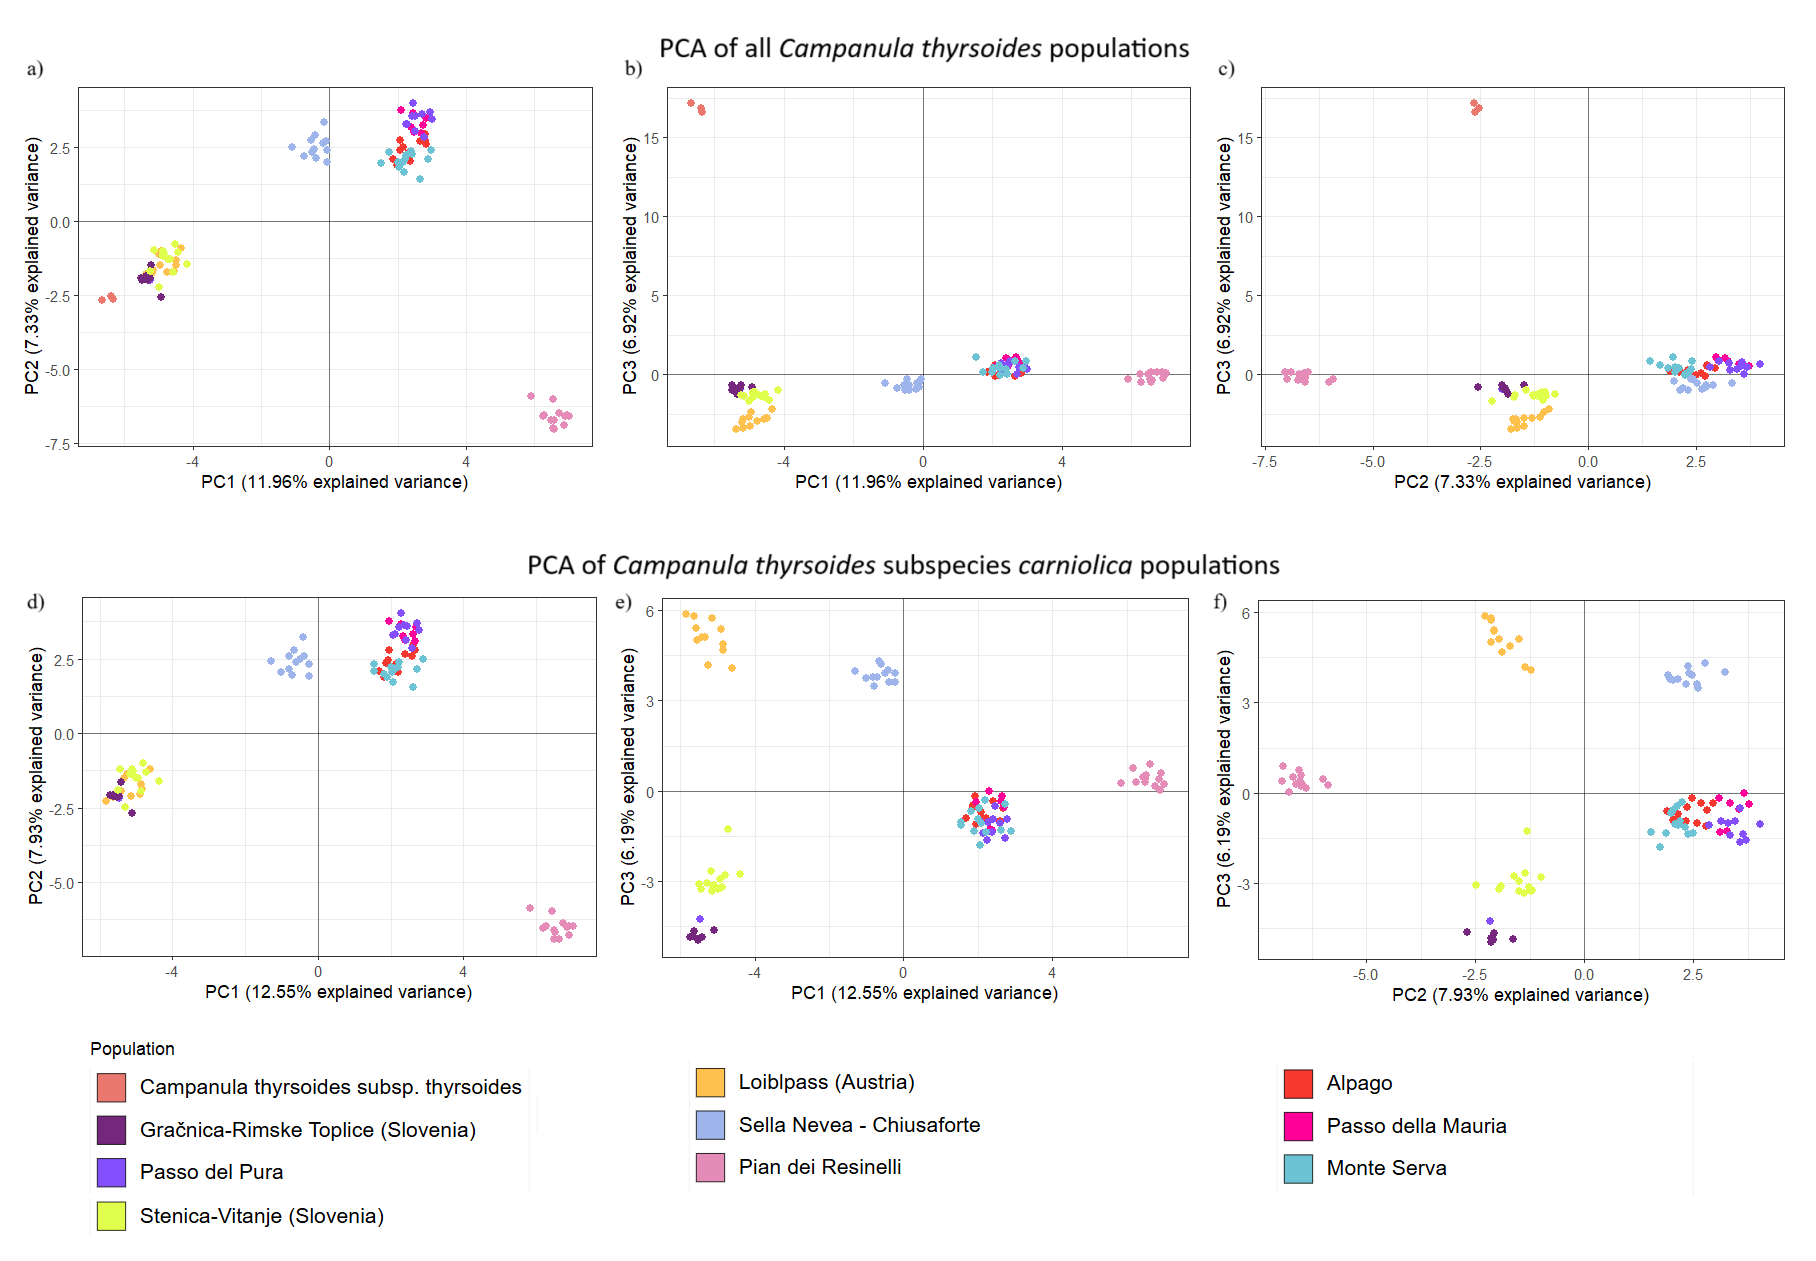
\includegraphics[width=1\linewidth]{PCA.png}
	\caption{\justifying{\footnotesize \textit{\textbf{PCA plots of \textit{Campanula thyrsoides} populations} \footnotesize{The PCA plots with all the populations (a, b, c) were built over 3896 polymorphic SNPs, while the plots portraying only populations of subspecies \textit{carniolica} (d, e and f) were based on 3558 SNPs.}}}}
	\label{fig:PCA}
\end{figure}

\subsubsection{Ancestry}
\vspace{-1em}
The ancestry shared by populations was assessed using phylogenetic trees and the programs \texttt{Admixture} and \texttt{STRUCTURE}. The consensus unrooted maximum likelihood phylogenetic tree (Fig. \ref{fig:unrooted}) effectively catches the big genetic distance of the outgroup CTT (subspecies \textit{thyrsoides}), whose clade separates from subspecies \textit{carniolica} with high support ($bootstrap = 100$) and was used to root the tree (Fig. \ref{fig:rooted}).  

\begin{figure}[h!]
	\centering
	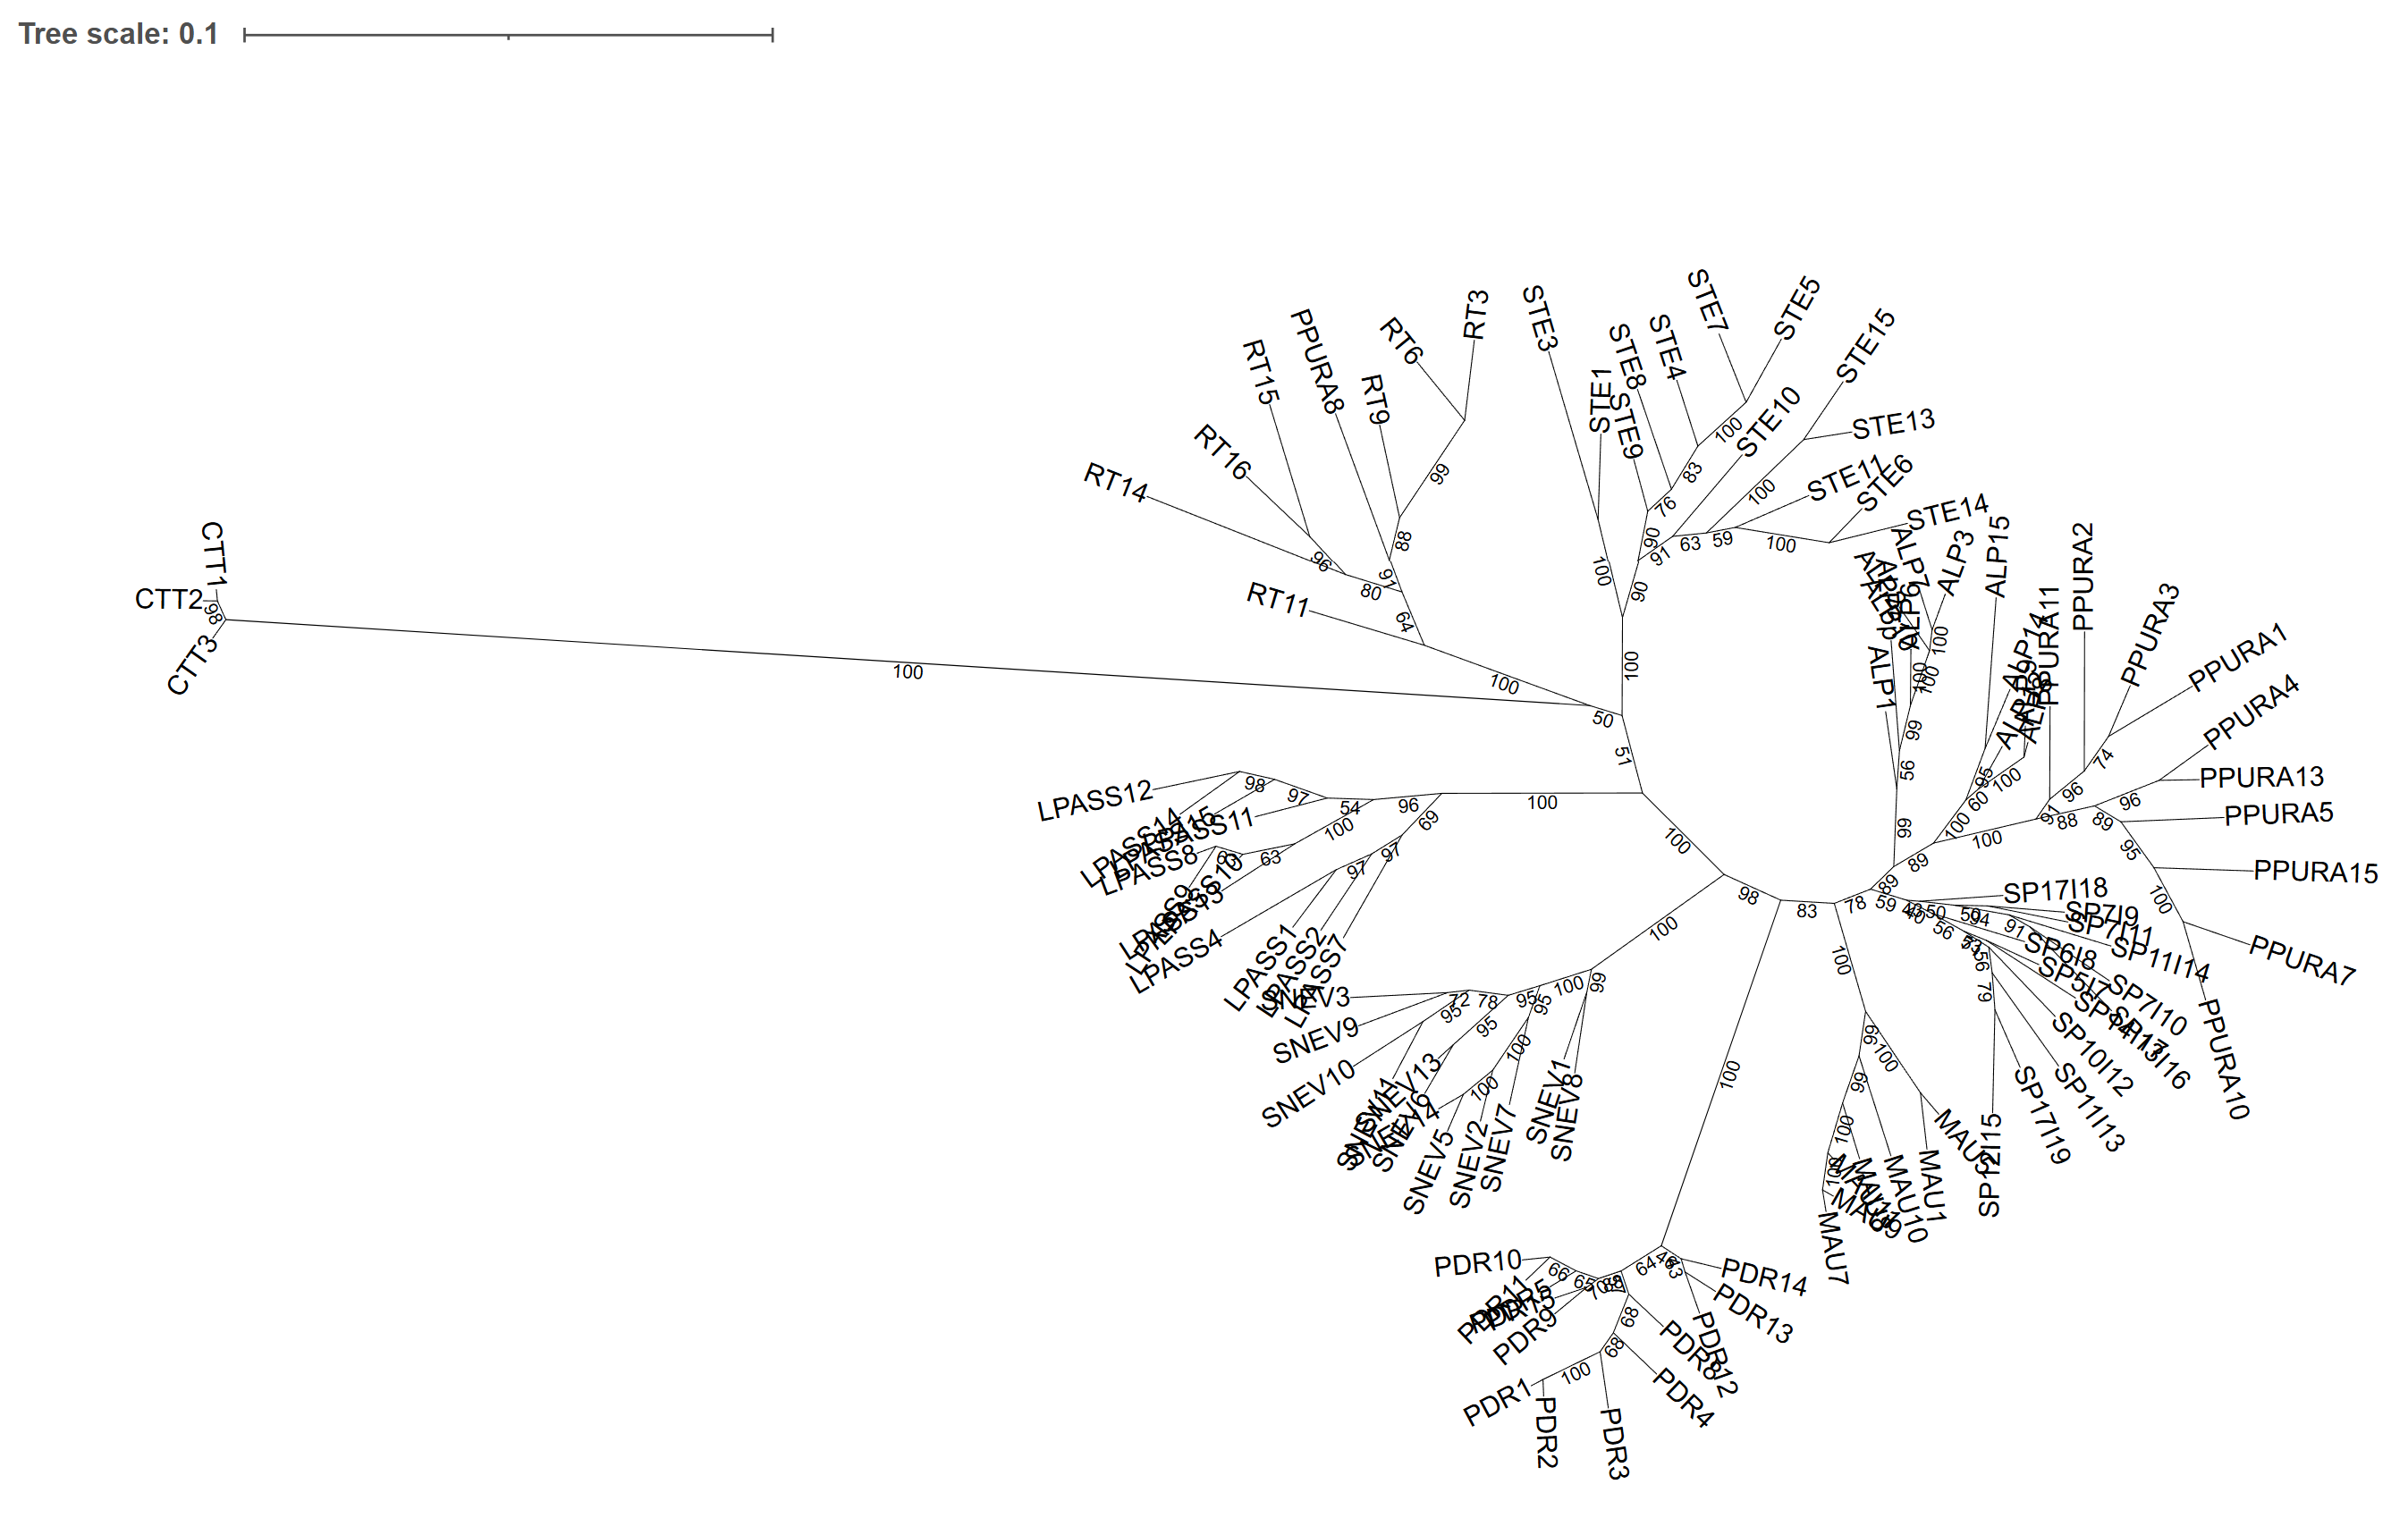
\includegraphics[width=0.85 \linewidth]{unrooted_campanula_qual.png}
	\caption{\justifying{\footnotesize \textit{\textbf{ML unrooted tree} \footnotesize{Consensus unrooted maximum likelihood phylogenetic trees constructed with \texttt{iqtree} and visualized with \texttt{iTOL} (v7; \cite{letunicInteractiveTreeLife2024}).}}}}
	\label{fig:unrooted}
\end{figure}

In the collapsed tree in Figure \ref{fig:rooted}, we can see that all populations clade bootstrap support is equal to $100$, with the exception of Monte Serva (SP) whose individuals group together with a weaker support (59) and Alpago (ALP) that instead forms two separated branches ($bootstrap = 99\text{-}100$). The separation between Slovenian populations and the others, is supported by weak boostrap values: for example, population RT separates with $boostrap = 50$ and STE with $boostrap = 51$. When the branch forms, though, both the Austrian population (LPASS) and the whole Italian clade (SNEV, PDR, MAU, SP, ALP, PPURA) diverge with perfect boostrap support ($bootstrap = 100$). It is interesting to notice, though, that the separation of RT and STE (Slovenia) together from the outgroup CTT is indeed evident (both $bootstrap = 100$): these observations confirm the clusters already appreciated in the PCA plots (Fig. \ref{fig:PCA}), where the Slovenian populations grouped together when CTT was involved (a, b, c) but separated well along PC3 when the outgroup was excluded (d, e, f). Coming back to the Italian populations, the tree highlights the difficulty in differentiating the populations from Veneto and Friuli Venezia Giulia, already noticed in the PCA: while in the PCA it is possible to separate SNEV when the outgroup is not involved (Fig. \ref{fig:PCA}, b versus e) this is not possible in the case of SP, ALP, PPURA and MAU. The phylogenetic tree is able to form different clades for each of them but the branches length is shorter in comparison to all the other populations, showing more vicinity between these samples.

\begin{figure}[h!]
	\centering
	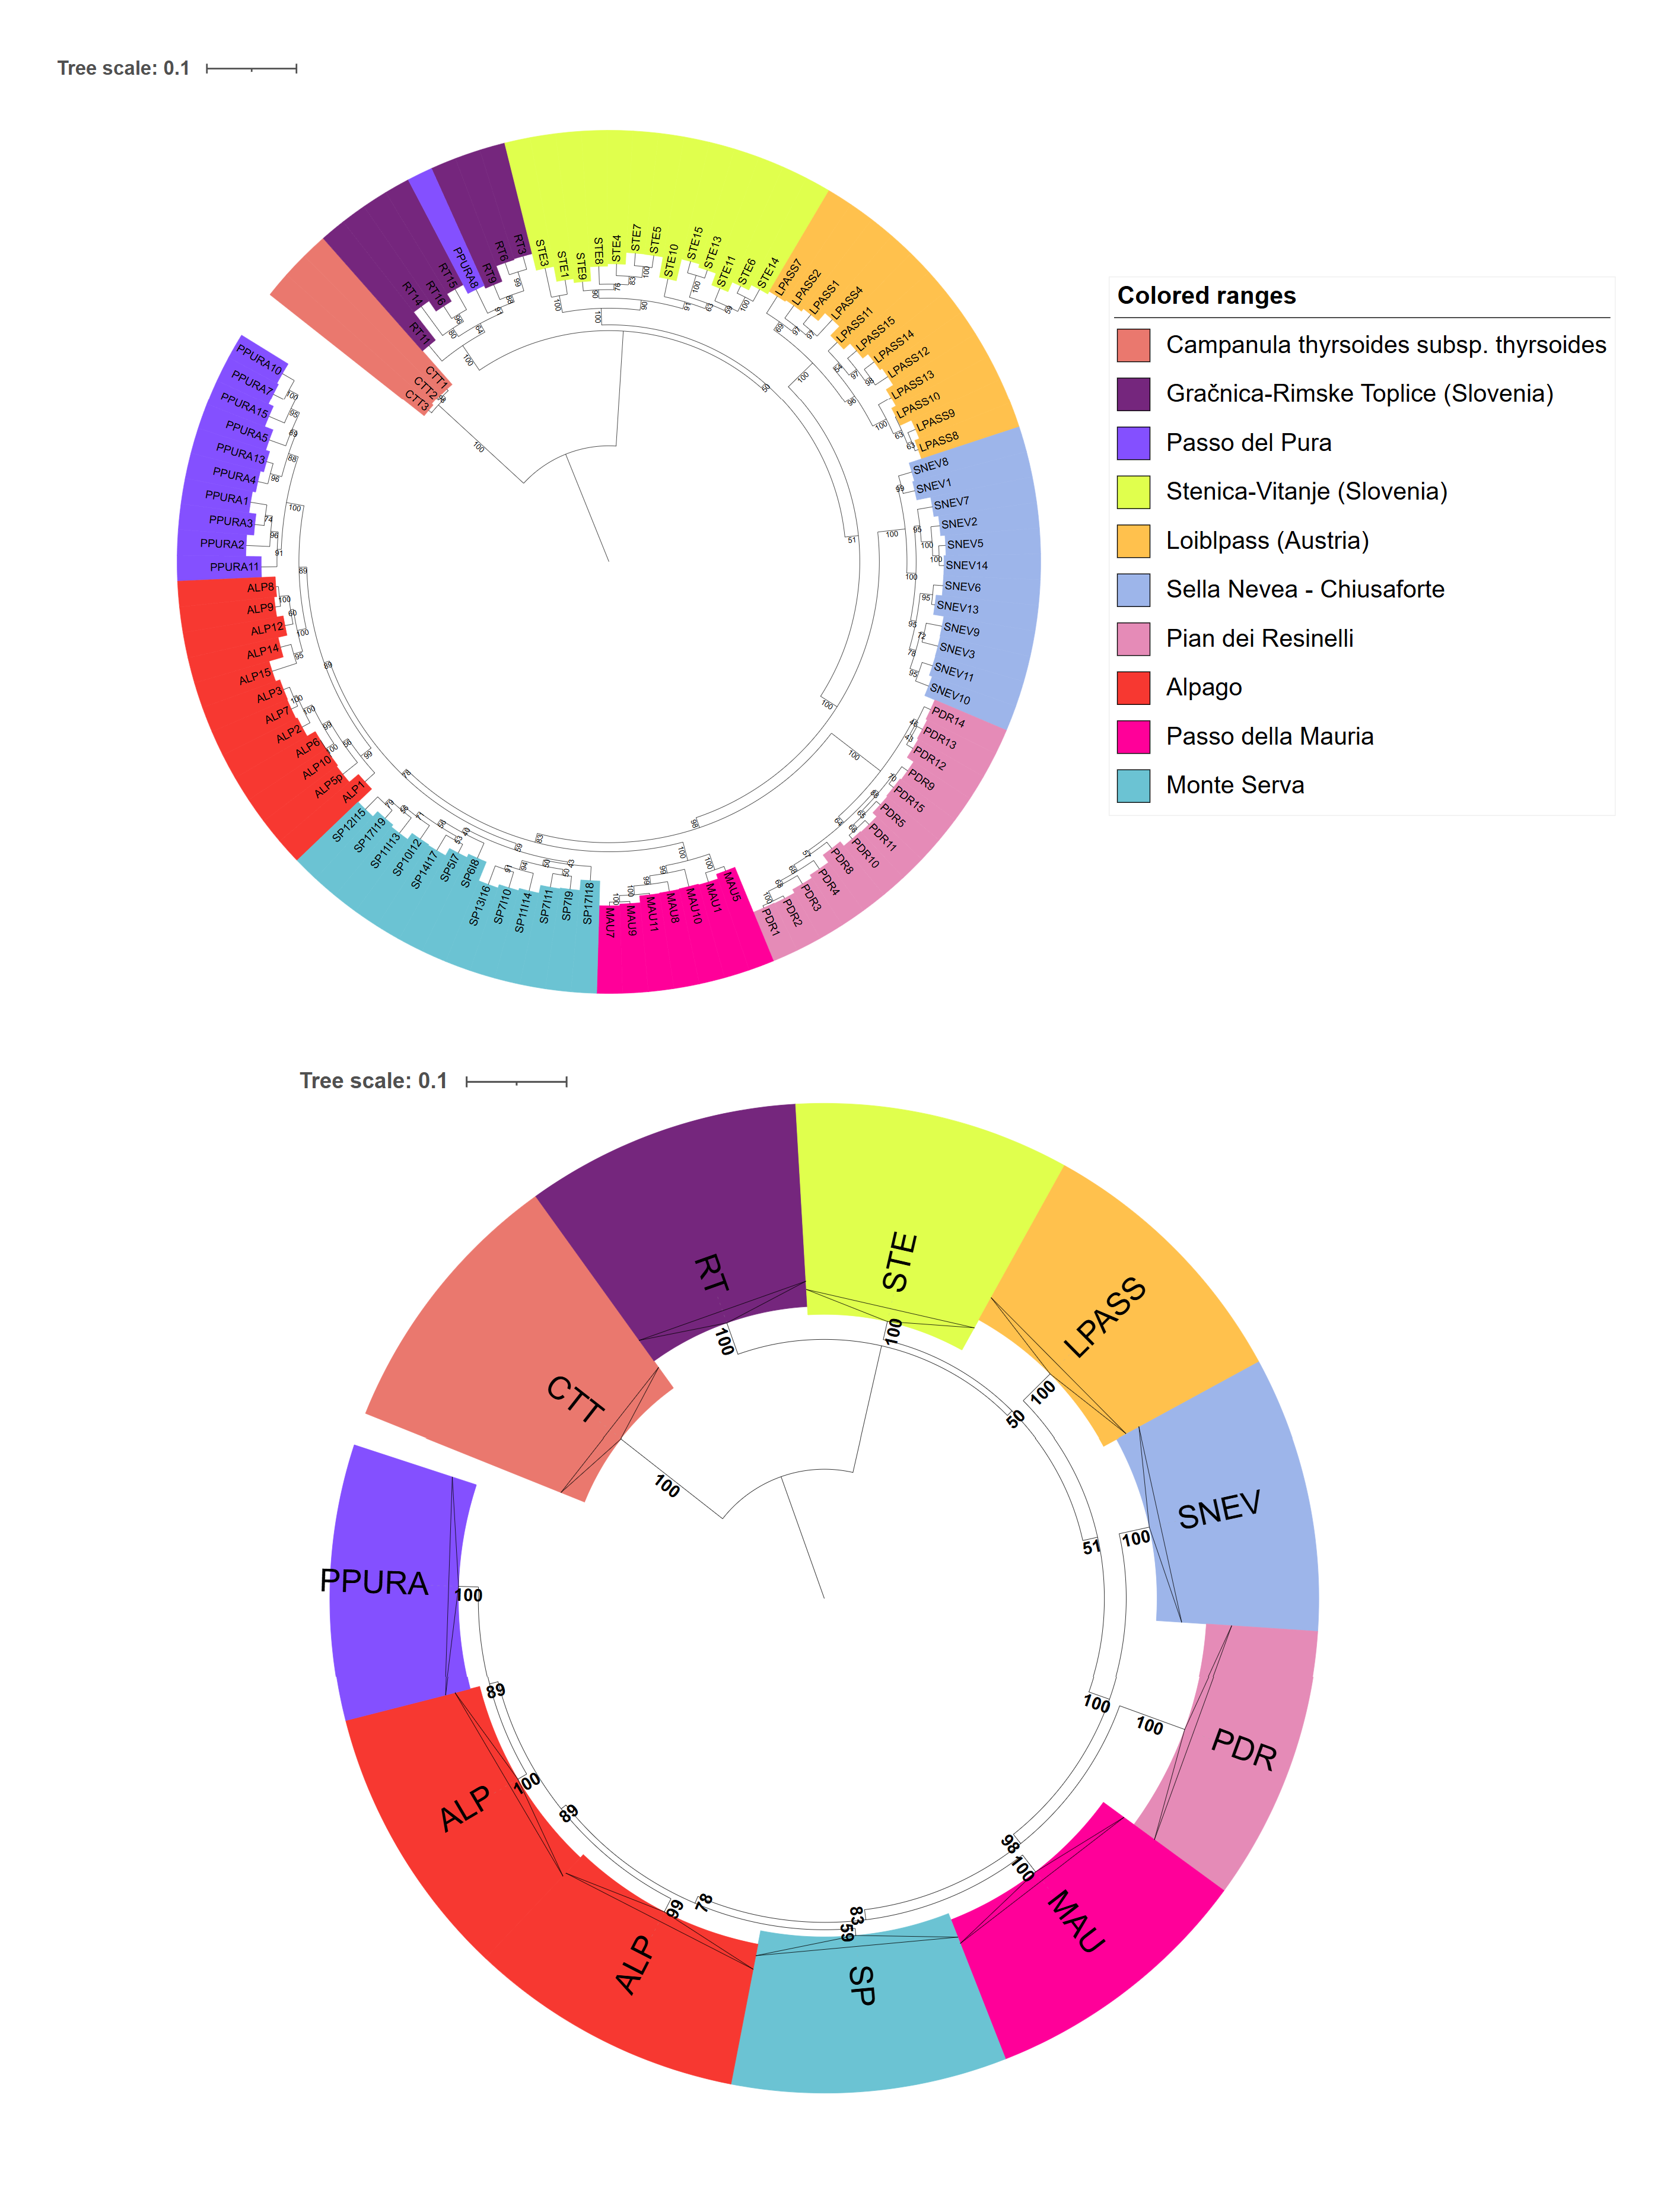
\includegraphics[width=0.80 \linewidth]{rooted_campanula_collapsed_and_not.png}
	\caption{\justifying{\footnotesize \textit{\textbf{ML rooted tree} \footnotesize{On the top, consensus maximum likelihood phylogenetic trees rooted on outgroup CTT clade, constructed with \texttt{iqtree} and visualized with \texttt{iTOL}. On the bottom, the same tree but with collapsed populations' clades for visualization purposes.}}}}
	\label{fig:rooted}
\end{figure}

%\begin{figure}[h!]
%	\centering
%	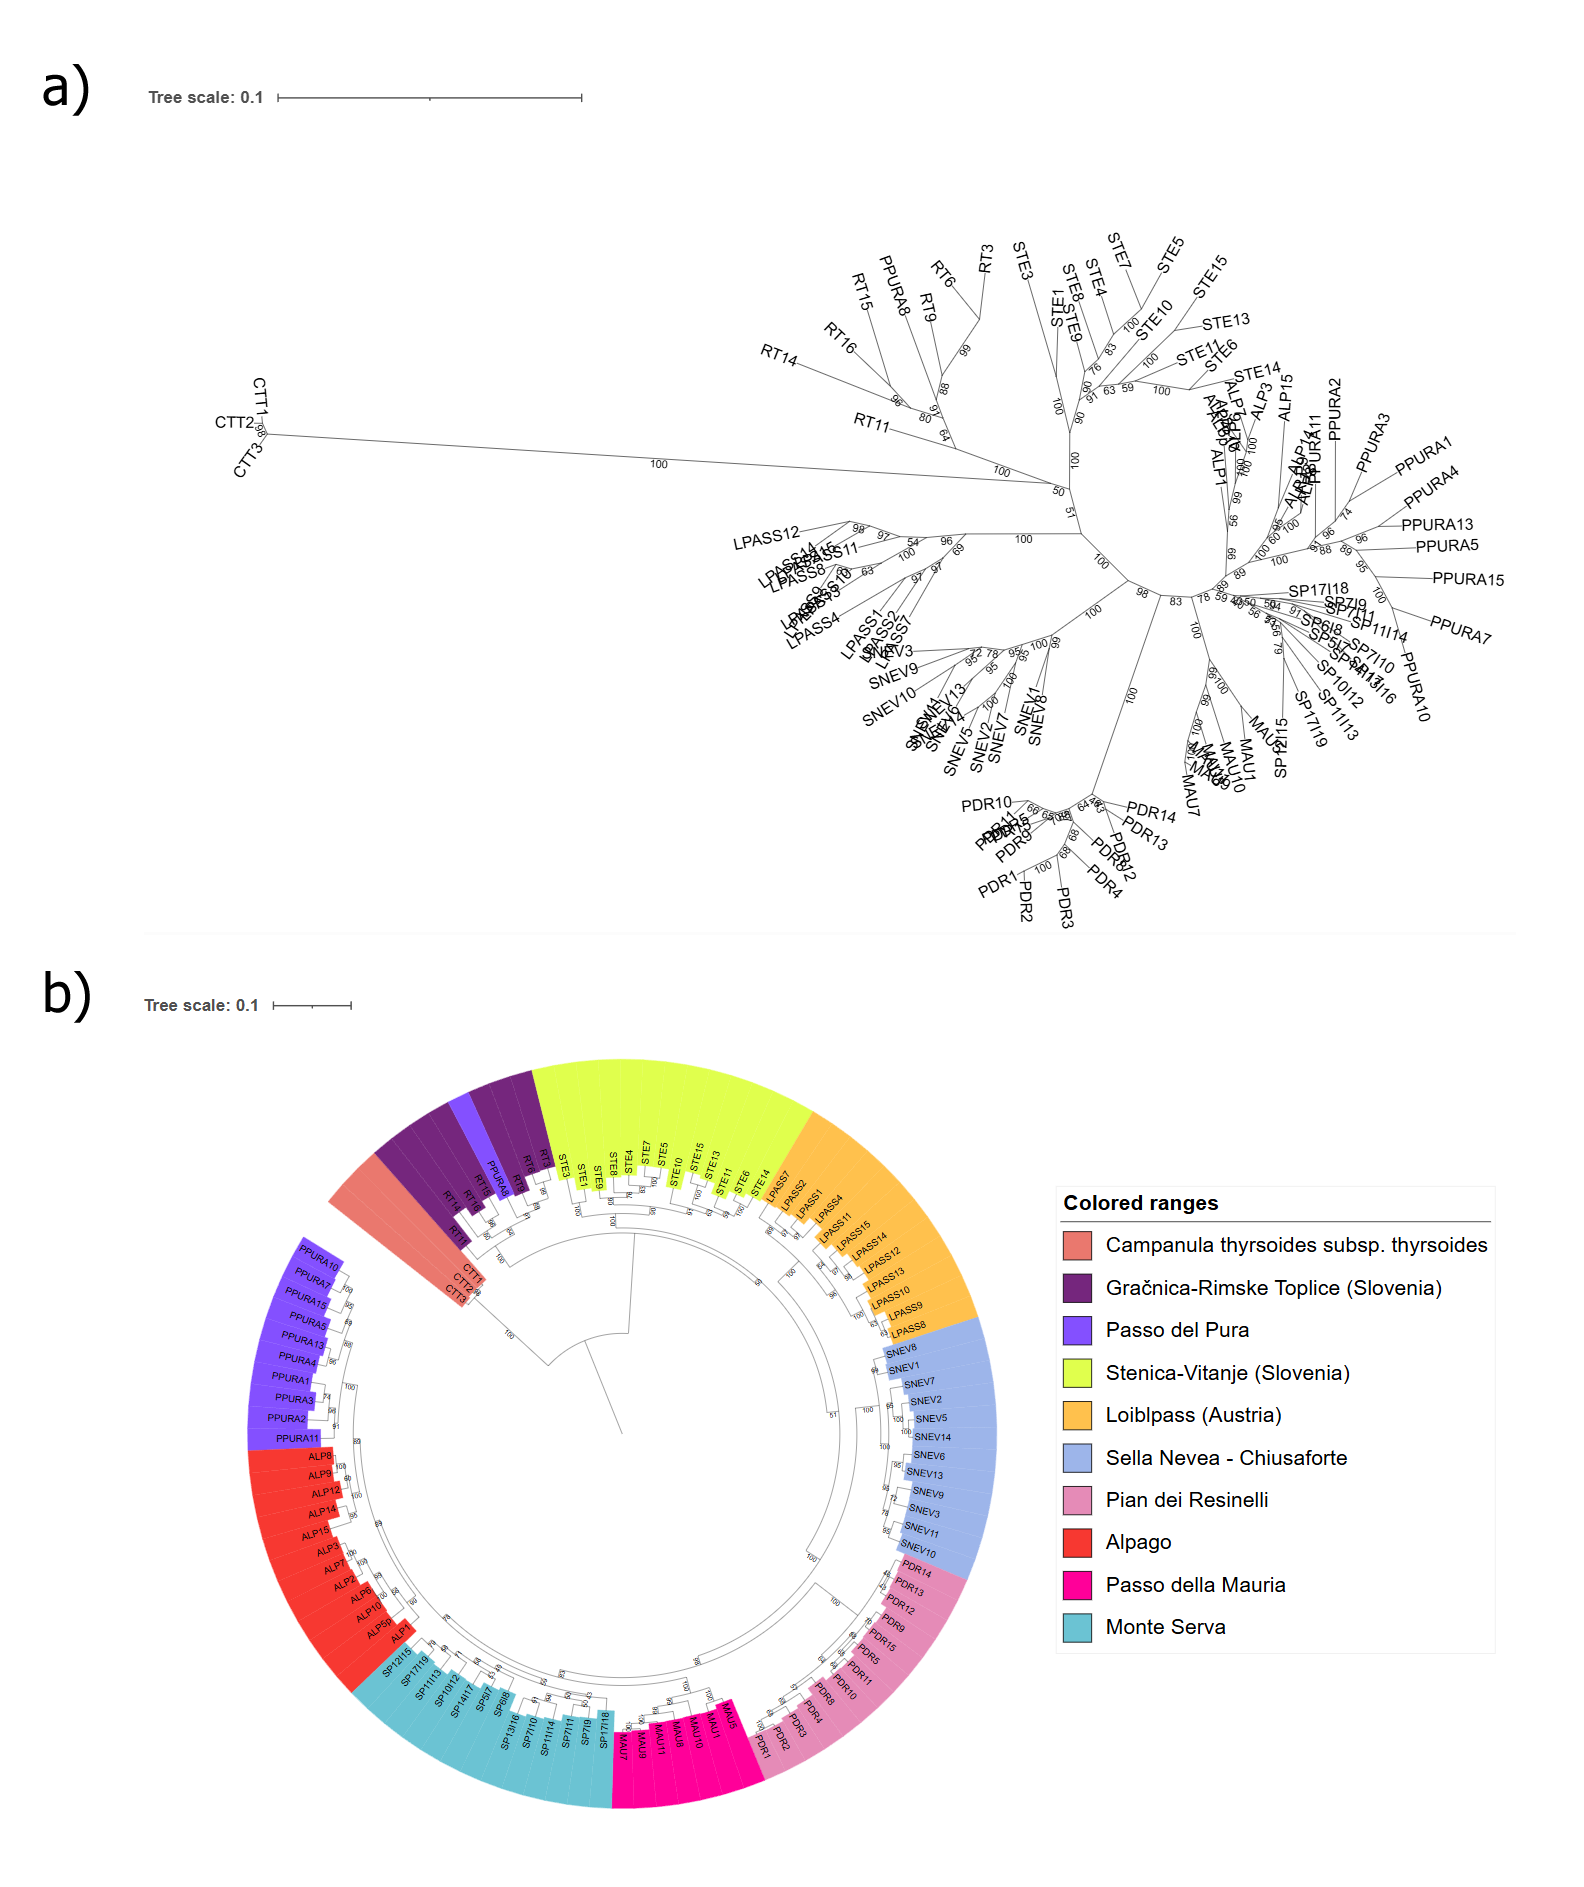
\includegraphics[width=1\linewidth]{alberi.png}
%	\caption{\justifying{\footnotesize \textit{\textbf{ML phylogenetic trees} \footnotesize{ (a) Consensus unrooted and (b) rooted on CTT population clade maximum likelihood phylogenetic trees constructed with \texttt{iqtree} and visualized with \texttt{iTOL}.}}}}
%	\label{fig:alberi}
%\end{figure}

With the use of  \texttt{STRUCTURE} it is possible to study in more detail the shared ancestry between samples, by separating them in artificial subpopulations. As already mentioned in the methods section, we first used program \texttt{Admixture} to quickly assess a large range of K values: by running the program with default parameters in a range of $K \in [2,30]$ we found that $K = 7$ had the minimum value of BIC error (Figure \ref{fig:BIC}). We then run program \texttt{STRUCTURE} in the neighbourhood of the optimal value $K = 7$ found by \texttt{Admixture},  so we tested for $K \in [1,20]$.

\begin{figure}[h!]
	\centering
	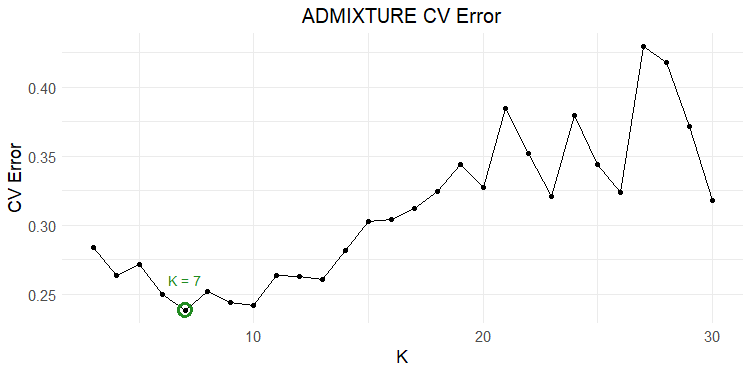
\includegraphics[width=0.70\linewidth]{CV_vs_K.png}
	\caption{\justifying{\footnotesize \textit{\textbf{\texttt{Admixture} cross validation error against K values} \footnotesize{Cross validation BIC error computed by \texttt{Admixture} to find the optimal K number of clusters. The minimum is found at $K = 7$.}}}}
	\label{fig:BIC}
\end{figure}

We employed both Evanno and Puechmaille methods to assess the best value of K: when including or excluding outgroup CTT, without exception, Evanno method found smaller optimal Ks (Figure \ref{fig:evanno}) both because of the goal of this method (find the highest hierarchical level) and because uneven sampling leads to a downward-biased estimate of K \parencite{puechmailleProgramStructureDoes2016}. This method is able to catch the differentiation between the two subspecies (when $K = 2$) and, when CTT is excluded, the subdivision of samples in Italian and not Italian, highlighting also the introgression of population ALP ($K = 3$). 

\begin{figure}[h!]
	\centering
	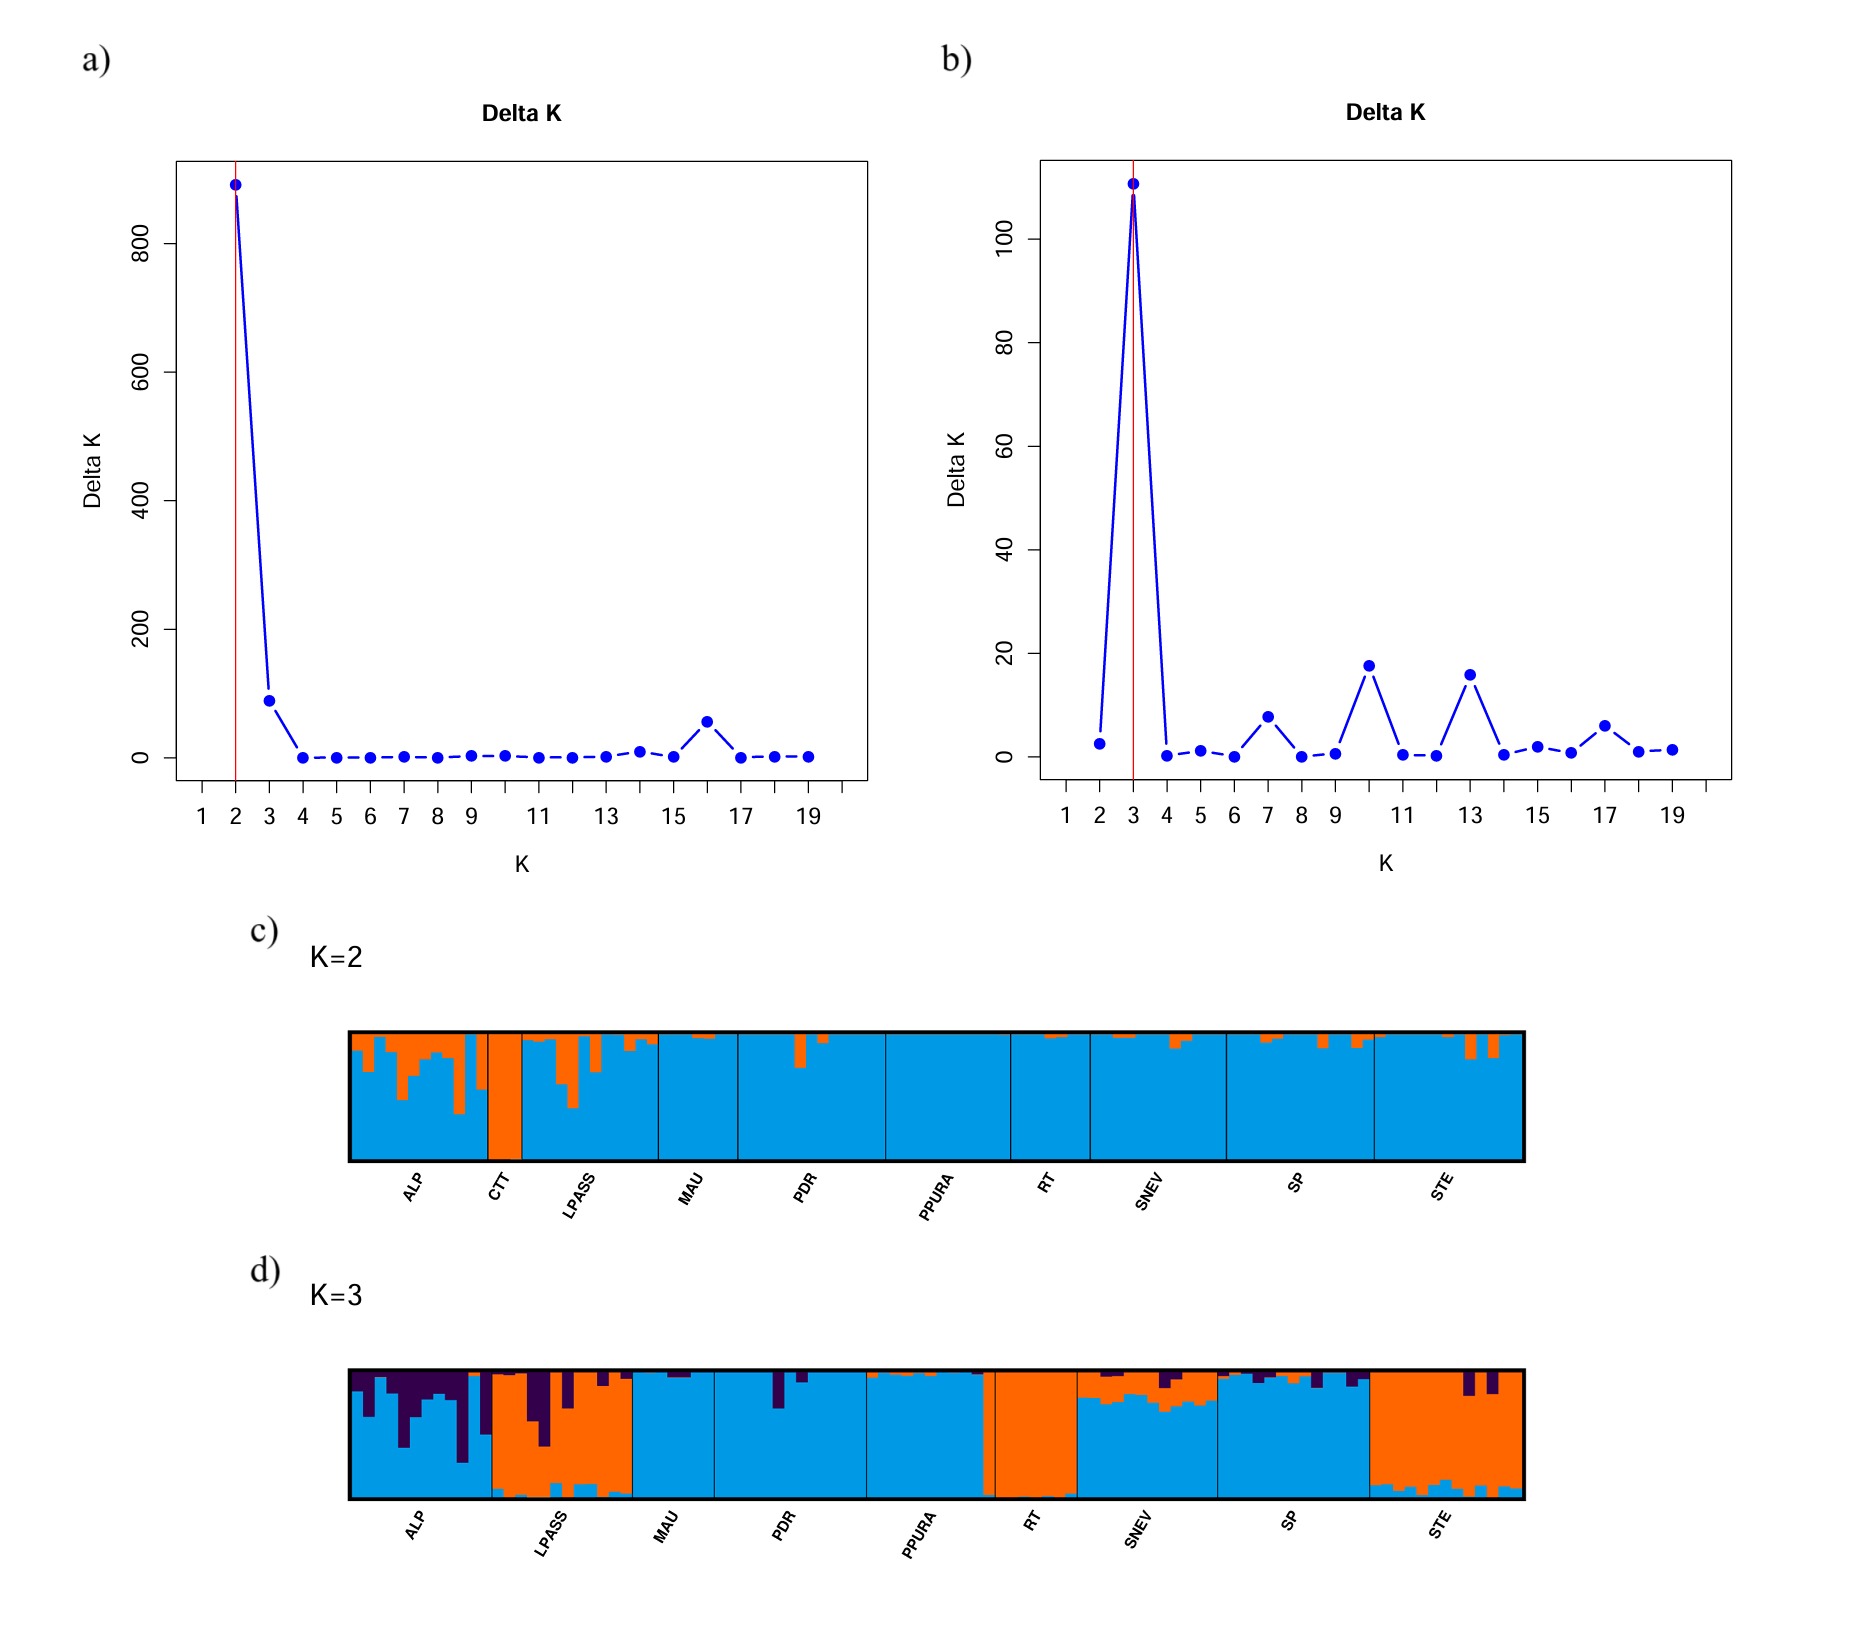
\includegraphics[width=0.70\linewidth]{Evanno_with_vs_without_CTT.png}
	\caption{\justifying{\footnotesize \textit{\textbf{Structure results (Evanno method).} \footnotesize{Results for \texttt{STRUCTURE} with (a) and without (b) outgroup CTT, using Evanno method to select the best number of K (maximum point) $\in [1,20]$ clusters. Visual representation offered by StructureSelector \parencite{liStructureSelectorWebbasedSoftware2018} and CLUMPAK \parencite{kopelmanClumpakProgramIdentifying2015}.}}}}
	\label{fig:evanno}
\end{figure}

Even if Puechmaille method performs better with uneven samples sizes \parencite{puechmailleProgramStructureDoes2016}, the comparison between the two methods can show interesting dataset characteristics. As shown in Fig.\ref{fig:structure}, when CTT is included the best K is always $K = 7$ while $K \in [6,7]$ otherwise.

\begin{figure}[h!]
	\centering
	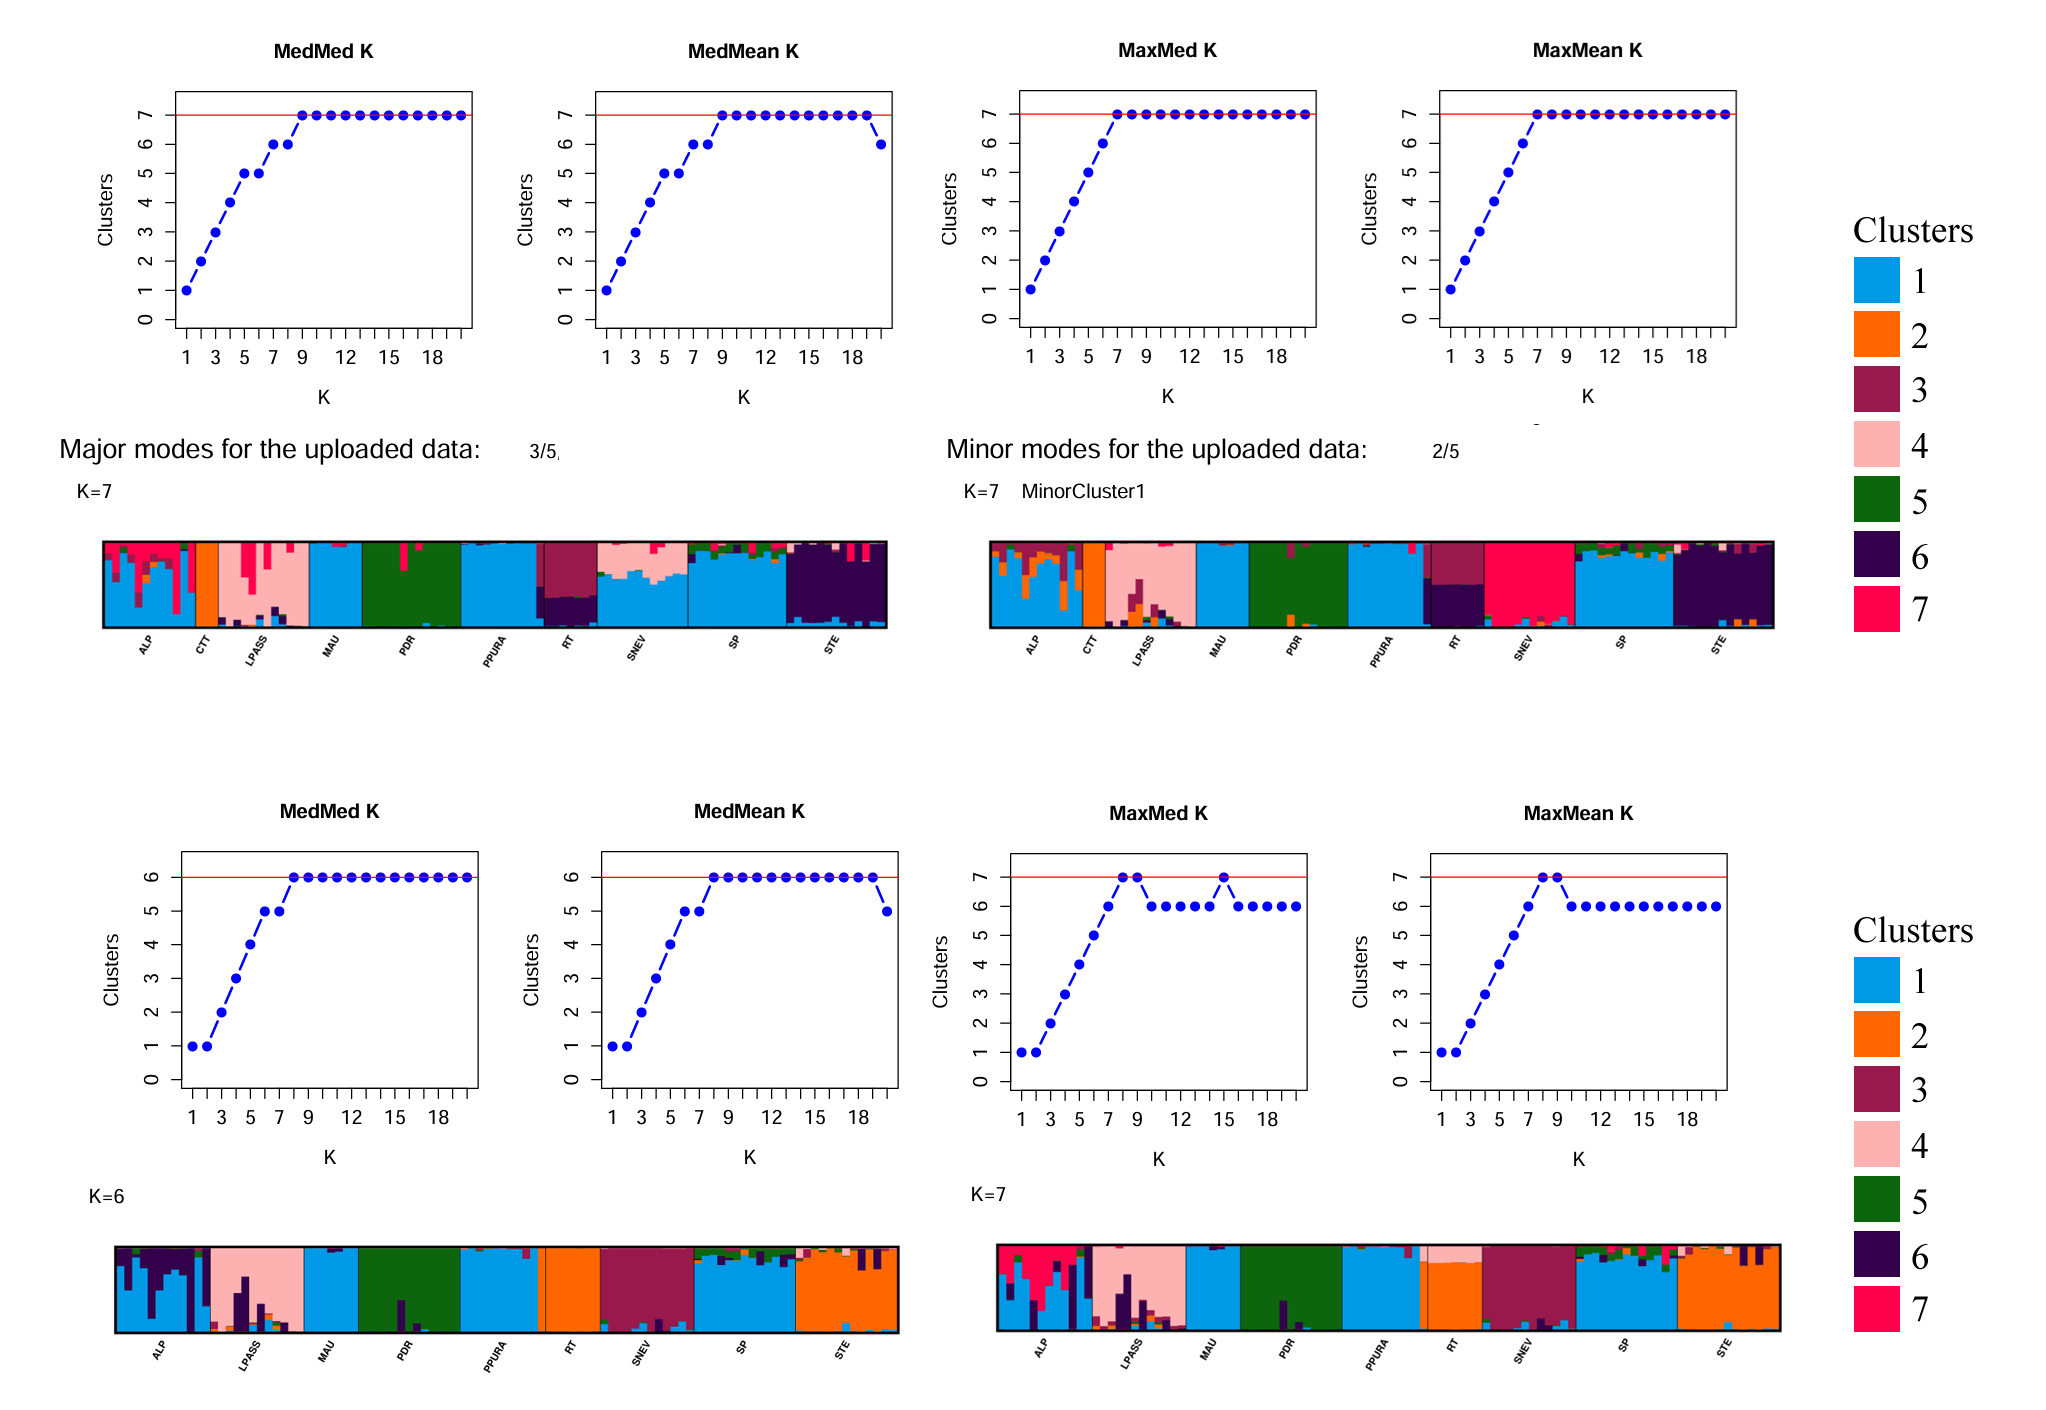
\includegraphics[width=1\linewidth]{Puechmaille_with_vs_without_CTT.png}
	\caption{\justifying{\footnotesize \textit{\textbf{Structure results (Puechmaille method).} \footnotesize{Results for \texttt{STRUCTURE} with (top) and without (bottom) outgroup CTT, using Puechmaille method to select the best number of K clusters. When CTT was involved, two main modes of clustering were equally represented (they're labelled as major and minor modes) so they are both shown in the figure. The maximum point in the plots corresponds to the optimal value of K. Visual representation offered by StructureSelector and CLUMPAK.}}}}
	\label{fig:structure}
\end{figure}

Differently from the findings in the PCA, when including CTT (top), the Slovenian populations do not easily cluster together (STE is part of cluster 6, and RT has admixed ancestry between cluster 3 and 6) while the exclusion of the outgroup makes RT and STE group under the same cluster 2 (bottom plots). This uncertainty in the two results is caught by the low bootstrap support in the consensus tree (Fig. \ref{fig:rooted}), which was discussed previously. In both cases, the populations SP, MAU and PPURA share the majority of their ancestry (cluster 1), while ALP shows a more fragmented ancestry while still being mainly part of cluster 1: this confirms the clustering of the Veneto and Friuli-Venezia-Giulia group. This group still excludes SNEV that shows some shared ancestry with the other four (cluster 1). Interestingly, when CTT is included (Fig. \ref{fig:structure}, top plots) in 3 runs out of 5 SNEV shares ancestry with both the Veneto-Friuli samples (cluster 1) and the Austrian ones (cluster 4). In the remaining 2 runs, this population shows no admixture (cluster 7) like it does when CTT is excluded (Fig. \ref{fig:structure}, bottom plots, where it belongs solely to cluster 3). This reflects the bootstrap value of 51 observed in the phylogenetic tree (Fig. \ref{fig:rooted}) on the branch separating LPASS from the Italian populations. Finally, because of PCA (Fig. \ref{fig:PCA}), phylogenetic trees (Fig. \ref{fig:rooted}) and \texttt{STRUCTURE} (Fig. \ref{fig:structure}) results we concluded the sample PPURA8 was actually a sample of population RT (Gračnica-Rimske Toplice, Slovenia) that got mis-labelled during DNA extraction. Since we could not confirm this theory we still kept it labeled as being part of PPURA population.


\subsubsection{Inbreeding metrics}
To assess within population diversity, we computed the inbreeding factor ($F_{IS}$) using R package \texttt{hierfstat}: this metric ranges from -1 (no inbreeding) to 1 (strong inbreeding). In Table \ref{tab:fis} we reported the 99.5\% confidence intervals we obtained from 9999 bootstrap iterations: none of the ranges contain 0, so we can confidently state no population suffers from inbreeding. In fact, all values are strongly negative, going from a minimum lower bound of $-0.76$ for population CTT to a maximum higher bound of $-0.31$ for PPURA. This confirms good genetic flow and no risk, at least currently, of inbreeding depression for any of the populations.

\begin{table}[h!]
	\centering
	\caption{\textbf{$F_{IS}$ 99.5\% confidence intervals for each population.}}
	\label{tab:fis}
	\begin{tabular}{lclc}
		\toprule
		\textbf{Pop} & \textbf{$C.I._{95\%}$} & \textbf{Pop} & \textbf{$C.I._{95\%}$} \\
		\midrule
		\textbf{ALP}   & $[-0.3784, -0.3419]$ & \textbf{PPURA} & $[-0.3501, -0.3152]$ \\
		\textbf{CTT}   & $[-0.7673, -0.7221]$ & \textbf{RT}    & $[-0.3823, -0.3497]$ \\
		\textbf{LPASS} & $[-0.4128, -0.3799]$ & \textbf{SNEV}  & $[-0.4266, -0.3903]$ \\
		\textbf{MAU}   & $[-0.4663, -0.4236]$ & \textbf{SP}    & $[-0.3645, -0.3286]$ \\
		\textbf{PDR}   & $[-0.5390, -0.4919]$ & \textbf{STE}   & $[-0.3651, -0.3337]$ \\
		\bottomrule
	\end{tabular}
	\caption*{\footnotesize{\textit{$F_{IS}$ 95\% confidence intervals estimated per population.}}}
\end{table}

To quantify between population diversity we computed pairwise $F_{ST}$ metric using R package \texttt{StAMPP}, which uses the formula by Weir and Cockerman \cite{weirEstimatingFStatisticsAnalysis1984} and corrected by Weir and Hill \cite{weirEstimatingFStatistics2002} for few, uneven and small populations sizes: the results are reported in Table \ref{tab:fst}. As seen before, MAU, ALP, SP and PPURA are close together, since they show low to moderate differentiation ($F_{ST} < 0.20$) with Monte Serva's population (SP) being the closest to ALP ($F_{ST} = 0.08$) and PPURA ($F_{ST} = 0.09$), which confirms what was already observed in the consensus tree (Fig. \ref{fig:rooted}). As expected, the population that is most genetically distant from the others is CTT ($0.50 < F_{ST} < 0.68$). We used these values for Isolation by Distance (IBD) testing, from which we excluded the outgroup samples CTT to better capture the pattern of geographical distribution of genetic diversity within subspecies \textit{carniolica}. 

\begin{table}[h!]
	\centering
	\caption{\textbf{Pairwise $F_{ST}$ (all p-values $< 10^{-16}$).}}
	\label{tab:fst}
	\begin{tabular}{lccccccccc}
		\toprule
		\textbf{Pop} & \textbf{ALP} & \textbf{CTT} & \textbf{LPASS} & \textbf{MAU} & \textbf{PDR} & \textbf{PPURA} & \textbf{RT} & \textbf{SNEV} & \textbf{SP} \\
		\midrule
		\textbf{CTT}   & 0.56 &       &       &       &       &       &       &       &       \\
		\textbf{LPASS} & 0.26 & 0.55  &       &       &       &       &       &       &       \\
		\textbf{MAU}   & 0.16 & 0.61  & 0.30  &       &       &       &       &       &       \\
		\textbf{PDR}   & 0.28 & 0.68  & 0.39  & 0.35  &       &       &       &       &       \\
		\textbf{PPURA} & 0.10 & 0.52  & 0.24  & 0.13  & 0.28  &       &       &       &       \\
		\textbf{RT}    & 0.27 & 0.50  & 0.25  & 0.30  & 0.40  & 0.22  &       &       &       \\
		\textbf{SNEV}  & 0.20 & 0.57  & 0.26  & 0.24  & 0.35  & 0.19  & 0.28  &       &       \\
		\textbf{SP}    & 0.08 & 0.54  & 0.24  & 0.14  & 0.26  & 0.09  & 0.24  & 0.19  &       \\
		\textbf{STE}   & 0.22 & 0.50  & 0.20  & 0.24  & 0.34  & 0.20  & 0.19  & 0.22  & 0.20  \\
		\bottomrule
	\end{tabular}
	\caption*{\footnotesize{\textit{Pairwise $F_{ST}$ values among populations. 
				The matrix is symmetrical; only the lower half is reported.}}}
\end{table}

IBD can be assessed employing the Mantel test which, as previously stated, can use Pearson, Spearman and Kendall correlation metrics. Following Table \ref{tab:correlation_metrics} we tested for Pearson's $r$ assumptions: no outliers, linearity and normality of data (Fig. \ref{fig:mantel}). We checked for the presence of outliers with means of a boxplot (Fig. \ref{fig:mantel}, a) and found none. To test for linearity we first visually inspected the residuals for homoscedasticity (Fig. \ref{fig:mantel}, b) and then used a Studentized Breusch-Pagan test with 1 degree of freedom, which null hypothesis ($H_0$) is that residuals are distributed with equal variance. Since we obtained p-value $= 0.3047$, we could not reject the null hypothesis, thus we confirmed presence of homoscedasticity. Lastly, we show QQ-plot of residuals (Fig. \ref{fig:mantel}, c) to check for normality, which is confirmed by Shapiro-Wilk normality test (p-value $= 0.6462$). Since all assumptions were met, we used Pearson metric and we found a strong correlation ($r = 0.817$, $\text{p-value} = 8\text{e-}04 $) between geographic and genetic distance. This also reflects the longitude gradient we observed qualitatively in the PCA.

\begin{figure}[h!]
	\centering
	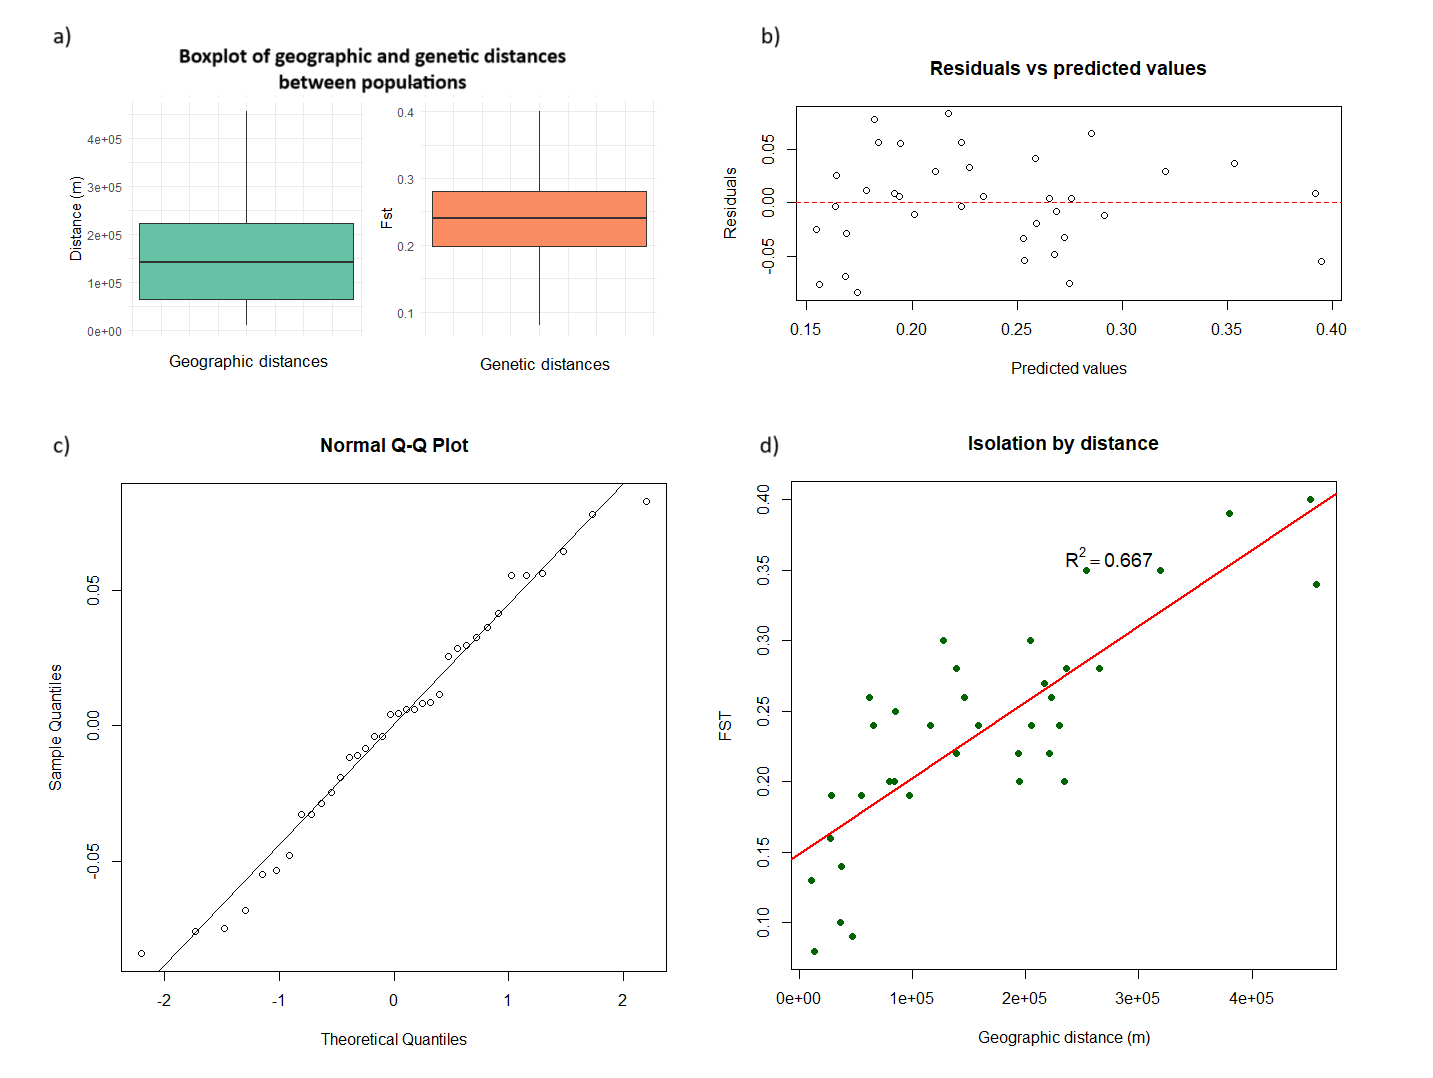
\includegraphics[width=1\linewidth]{mantel_test_assumptions.png}
	\caption{\justifying{\footnotesize \textit{\textbf{Mantel test assumptions and results} \footnotesize{To employ Pearson's correlation in the Mantel test, we checked the presence of outliers (a) and tested for linearity (b) and normality (c) of residuals. In (d) the scatterplot of data (in green) with the regression line (red) corresponding to model $F_{ST} = 1.488\text{e-01} + 5.384\text{e-07} \cdot \text{distance}$ ($R^2 = 0.6576$, $\text{p-value} = 1.222\text{e-09}$).}}}}
	\label{fig:mantel}
\end{figure}

\subsubsection{Comparison of software for $F_{ST}$ estimation}
Although we ultimately used the $F_{ST}$ values as computed by package \texttt{StAMPP}, we tested 2 software and 2 R packages as well, in order: \texttt{stacks}: \texttt{populations}, \texttt{vcftools}, \texttt{BEDASSLE} and \texttt{hierfstat}. They can be roughly separated depending if they estimate an unweighted (Group 1: \texttt{populations}, \texttt{hierfstat} and unweighted \texttt{vcftools}) or weighted $F_{ST}$ value (Group 2: weighted \texttt{vcftools}, \texttt{BEDASSLE}, \texttt{StAMPP}): within their group, all software perform similarly, but the difference between the two formulas is noticeable when observing the color scale of the heatmaps of their results (Figure \ref{fig:heatmapfst}). We grouped together the software in the aforementioned groups and computed the average $\bar{F}_{ST}^{\text{Group}}$ for each pair of populations. Then we performed a Wilcoxon paired test, with 
$H_0: \bar{F}_{ST}^{\text{Group 1}} = \bar{F}_{ST}^{\text{Group 2}}$ 
and 
$H_A: \bar{F}_{ST}^{\text{Group 1}} < \bar{F}_{ST}^{\text{Group 2}}$. 
There is statistical significance showing that the software using unweighted estimates of $F_{ST}$ obtain lower values than those that use the weighted formula (p-value $= 2.842\cdot 10^{-14}$). 

\begin{figure}[h!]
	\centering
	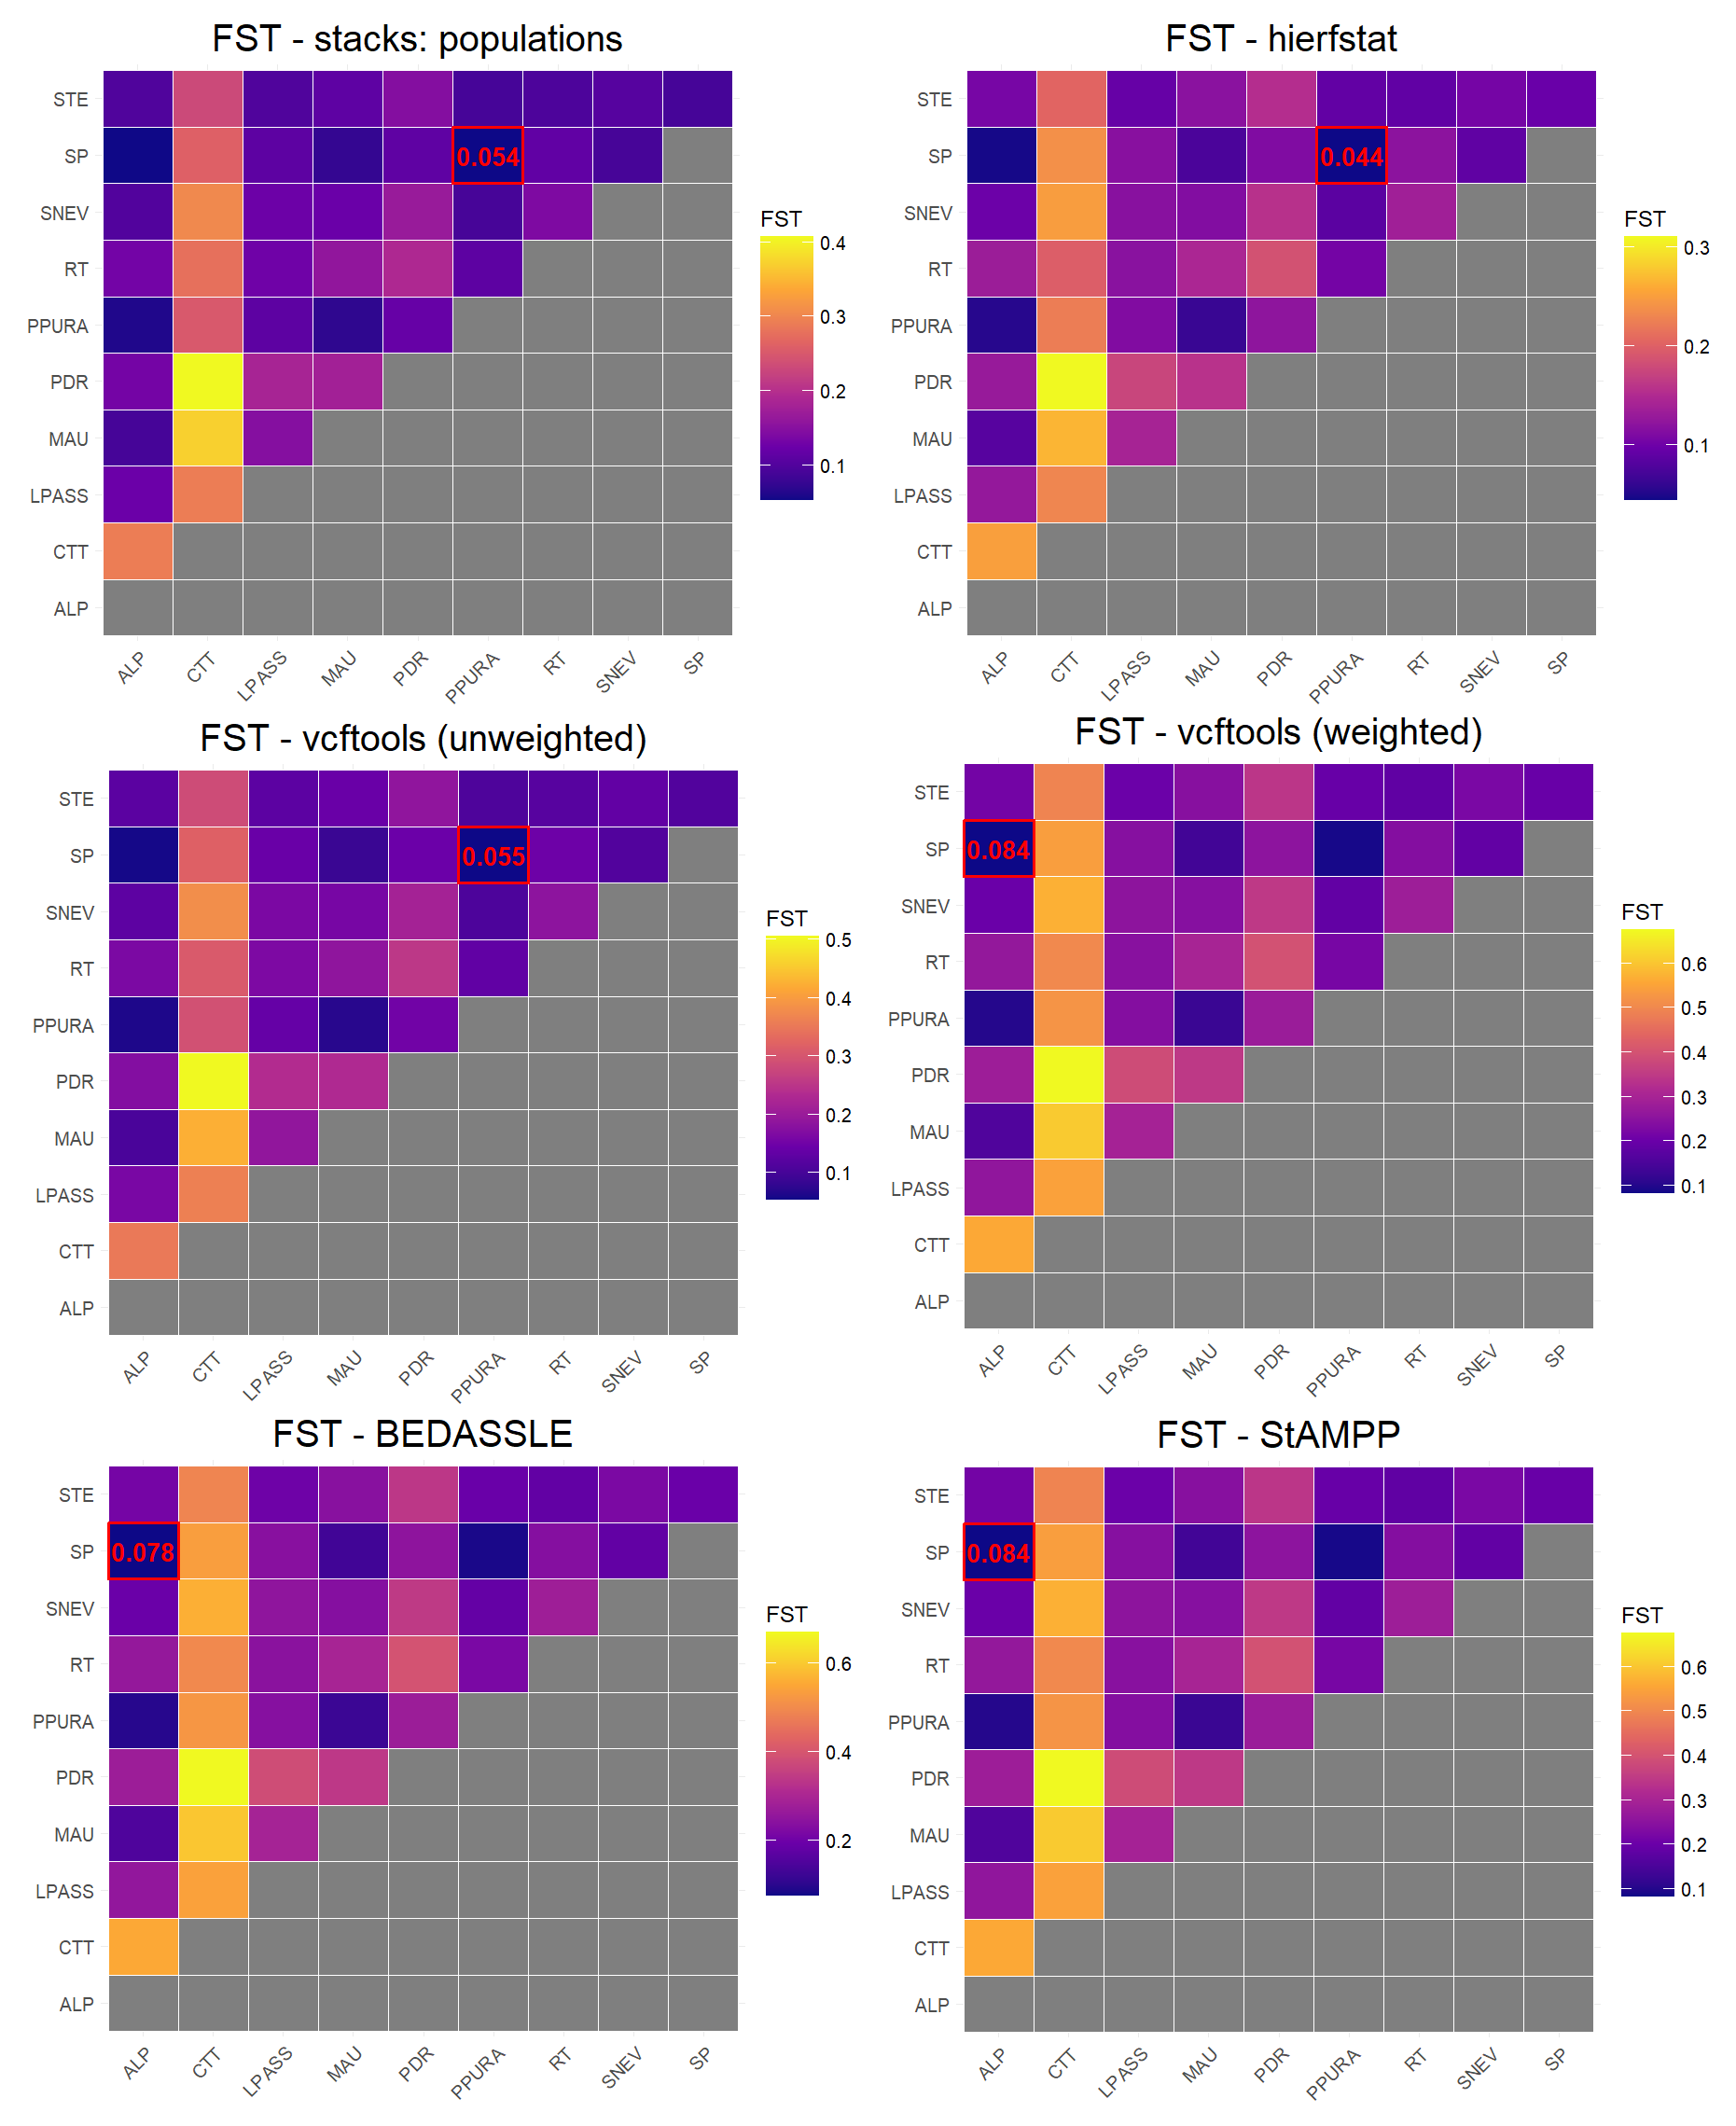
\includegraphics[width=1\linewidth]{heatmap_fst2.png}
	\caption{\justifying{\footnotesize \textit{\textbf{Heatmaps of software estimates of $F_{ST}$} \footnotesize{We compare software performance by plotting heatmaps of $F_{ST}$ estimates for each software tested. In red, the lowest value for Monte Serva population (SP), target of the study.}}}}
	\label{fig:heatmapfst}
\end{figure}

Group 1 always underestimated the results in comparison to Group 2: despite the difference in absolute values, this shows that the relationships between populations (computed as the genetic distance between each other) behaved consistently. Populations that are closer in comparison to others, remain the same even if another software is employed to estimate this quantity. It is the absolute value of this distance that changes, but in the case of close populations the difference is minimal: for example, the population closest to the target population SP (Monte Serva) changes when using unweighted (PPURA) or weighted estimates (ALP) but this divergence is not alarming, since PPURA is the second-lowest result for weighted estimates, and ALP for the unweighted ones. 

The situation is slight different when considering distant populations: for example, the outgroup CTT, when using unweighted estimates, is the furthest from PDR with $F_{ST} = 0.51$ in (unweighted) \texttt{vcftools}. As shown by all the software in Group 2, it is still the most distant from PDR, but the value is as large as $F_{ST} = 0.68$ in \texttt{StAMPP}: a difference of $0.17$ in other analysis could easily lead to two very distinct conclusions. Nevertheless, we believe that \texttt{StAMPP} was the best choice for our analysis, both considering the assumptions already discussed in the Material and Methods Chapter, and its ability to compute the associated p-values. The two other weighted estimates software also have their advantages: R package \texttt{BEDASSLE}, similarly to \texttt{StAMPP}, is able to compute confidence intervals, which can give insight on the strength of its results. And \texttt{vcftools}, which is a software that many researchers are already familiar with, is able to operate on the terminal and with faster computations, so \texttt{.vcf} files do not need to be exported and converted to the appropriate input format which R packages expect.

\clearpage
\section{\textit{Solanum tuberosum} landraces}
We performed variant calling for the genus \textit{Solanum}, with broadly the same pipeline used for Campanula but accounting for the presence of a reference genome. The final \texttt{.vcf} file contained 14,940 SNPs, and only one sample had more than 20\% missing data (the sample OL\_PIET, Oltrepò di Pietragavina, with 23.2\% missing data), while the rest had less than 10\% (Fig. \ref{fig:missing_potatoes}).

 \begin{figure}[h!]
	\centering
	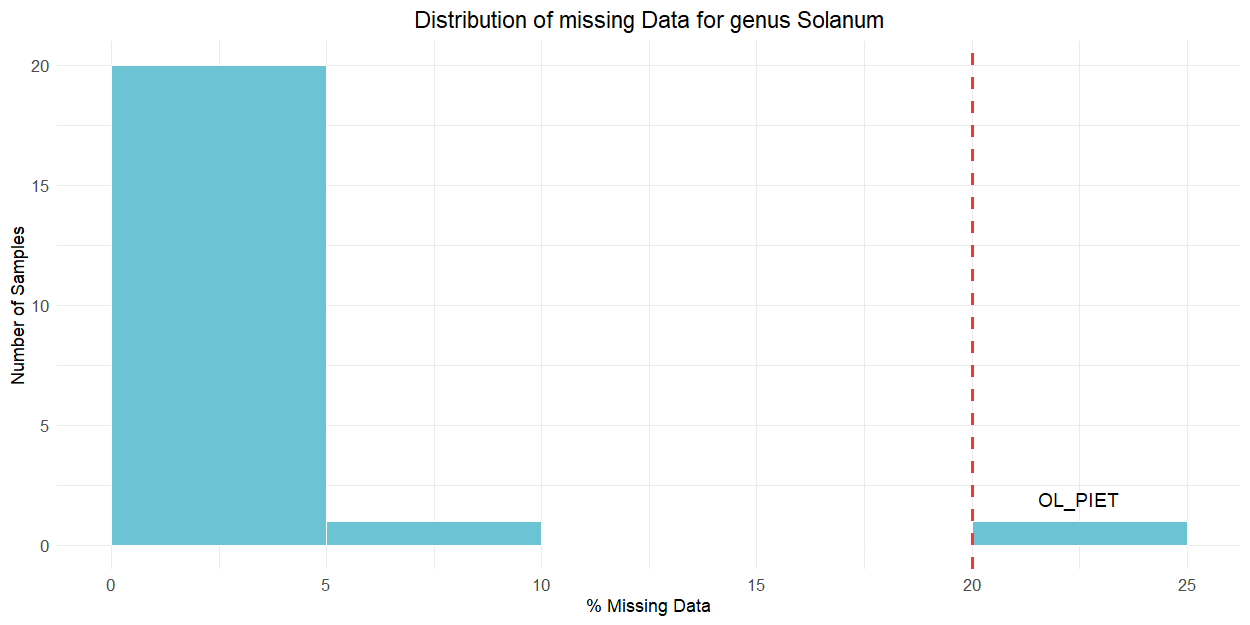
\includegraphics[width=0.80\textwidth]{percent_missing_potatoes.png}
	\caption{\justifying{\footnotesize \textit{\textbf{Missing data distribution of \textit{Solanum} genus' samples.} \footnotesize{This barplot shows the distribution of the missing data (in percentage) over 14,940 SNPs: a threshold of 20\% is highlighted by a vertical red line.}}}}
	\label{fig:missing_potatoes}
\end{figure}

When we included all the ancient and wild species, the PCA plots were built on 14,940 SNPs (Fig. \ref{fig:pca_patate}, a). Instead, when we excluded all the ancient/wild species and we used only \textit{S. tuberosum} subsp. \textit{andigenum} as the outgroup, the final matrix contained 10,496 SNPs  (Fig. \ref{fig:pca_patate}, b, c and d). When including all the species (Fig. \ref{fig:pca_patate}, a), the first principal component, explaining 27.6\% of the variance, is able to catch the division between cultivated and wild species, distinction reported in Table \ref{tab:solanum}. In fact, cultivated species are all distributed towards negative values of the x axis, with the cultivated Andean species grouping together in the Cluster A and all commercial cultivars and landraces in Cluster C, and \textit{S. tuberosum} subsp. \textit{andigenum} located between clusters A and C. All the wild species group together in cluster B towards positive values of the x axis, distant from cultivated species. When, out of all the control species, only \textit{S. tuberosum} subspecies \textit{andigenum} is plotted, the first PC (20.25\% of variance explained) catches the division between white and red peel potatoes. Furthermore, Cluster C separates in Cluster D (white peel potatoes close to commercial cultivar Kennebec) and Cluster E (red peel potatoes close to commercial cultivar Desiree). One landrace, Bianca (in yellow) is placed towards the middle point between white and red peel landraces. Obsolete cultivars (Bossico and Shilpario) and Starleggia Bianca do not cluster with all the other landraces, placing themselves between \textit{S. tuberosum} subsp \textit{andigenum} and cluster D (along PC2, Fig. \ref{fig:pca_patate}, b).

 \begin{figure}[h!]
	\centering
	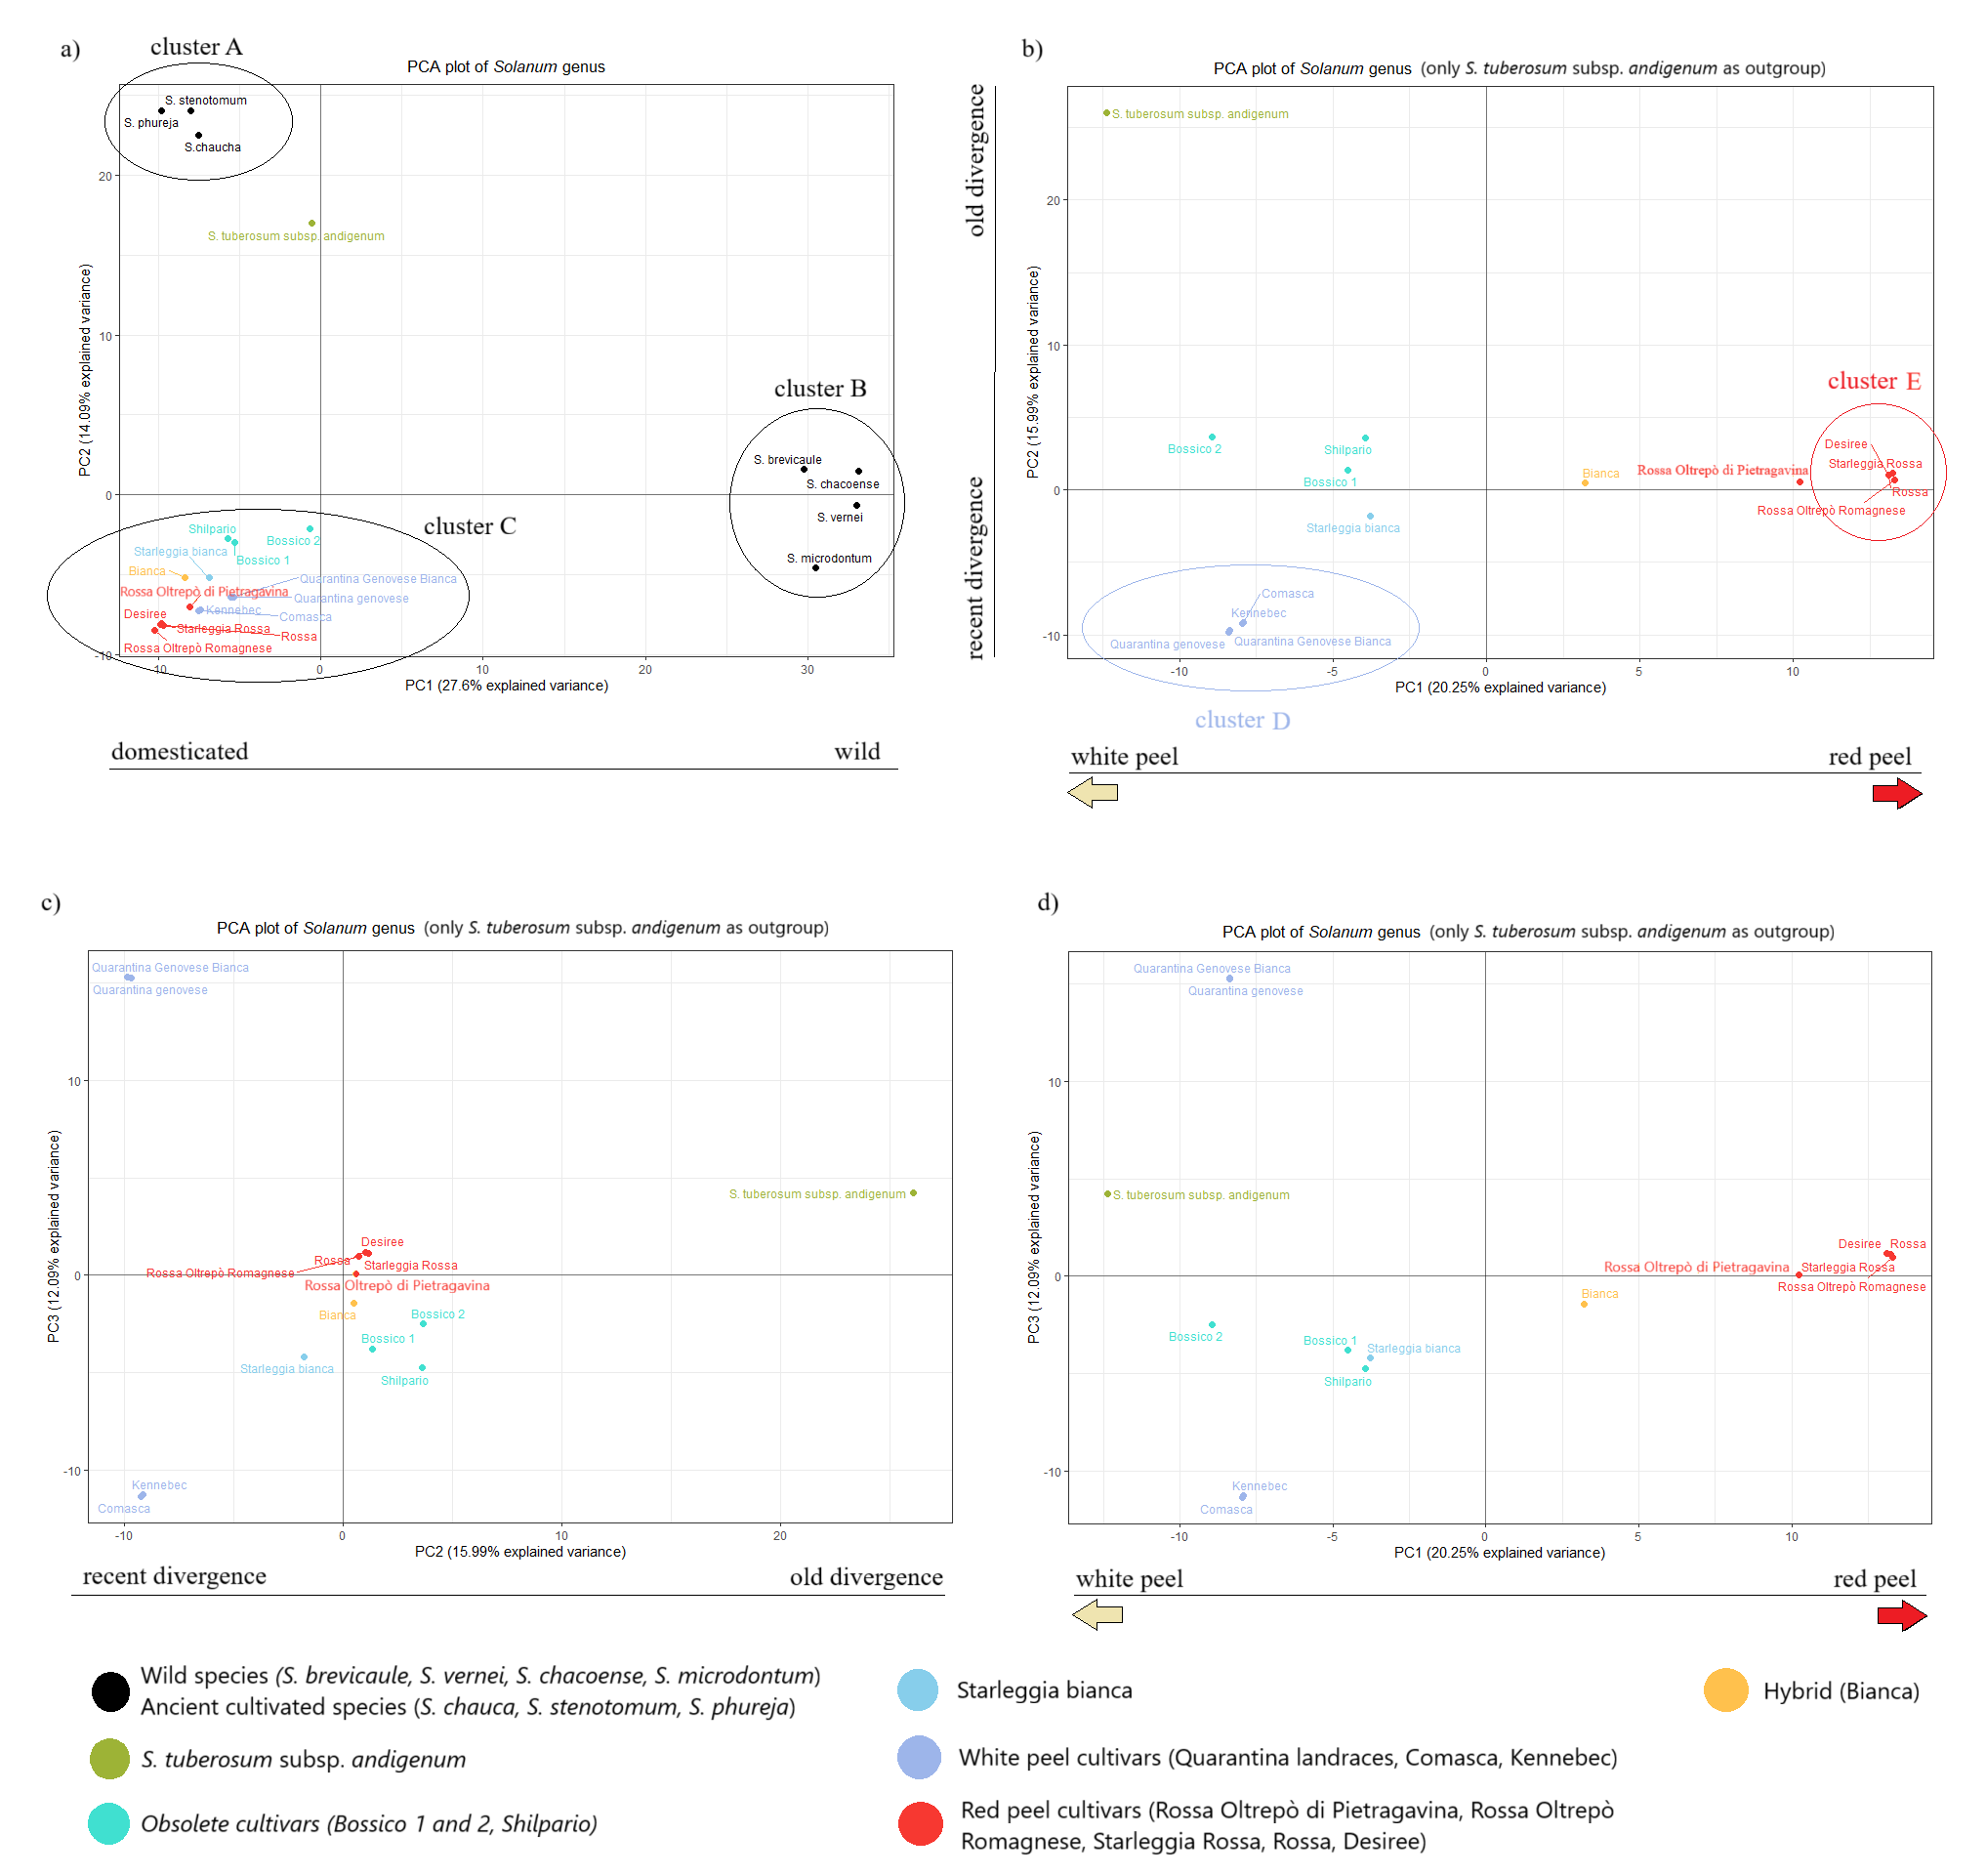
\includegraphics[width=1\textwidth]{PCA_patate.png}
	\caption{\justifying{\footnotesize \textit{\textbf{\textit{Solanum} genus samples' PCA plots.} \footnotesize{PCA plots of either (a) all \textit{Solanum} genus samples in the study or (b, c, d) only landraces and \textit{S. tuberosum} subsp. \textit{andigenum} as outgroup. Please refer to the legend to distinguish the samples: (i) black: wild/ancient species, (ii) green: \textit{S. tuberosum} subsp. \textit{andigenum}, (iii) cyan: obsolete landraces (Bossico and Shilpario), (iv) light blue: Starleggia Bianca, (v) blue: white peel landraces close to commercial Kennebec, (vi) red: red peel landraces close to commercial Desiree, (vii) yellow: hybrid landrace Bianca.}}}}
	\label{fig:pca_patate}
\end{figure}

To better appreciate the variance (15.99\%) caught by PC2 (Fig. \ref{fig:pca_patate}), we can integrate the information coming from the maximum likelihood phylogenetic tree, built as illustrated in the Methods section. In the unrooted tree (Figure \ref{fig:unroteed_patate}), it is again possible to see an evident division between wild species and cultivated species/landraces, found at opposite ends of the tree: the former are located on the left branches, while the latter on the right\footnote{Left and right are relative to this specific tree which was plotted using the web tool iTOL, with custom rotation for visualization purposes.}. It also shows that wild species, in green, grouped with high support ($bootstrap = 100$) and a big genetic distance, reflected by the length of the branch, from the rest of the samples. This guided our choice of rooting the tree on this clade (Fig. \ref{fig:albero_patate}), considering them as outgroup.

 \begin{figure}[h!]
	\centering
	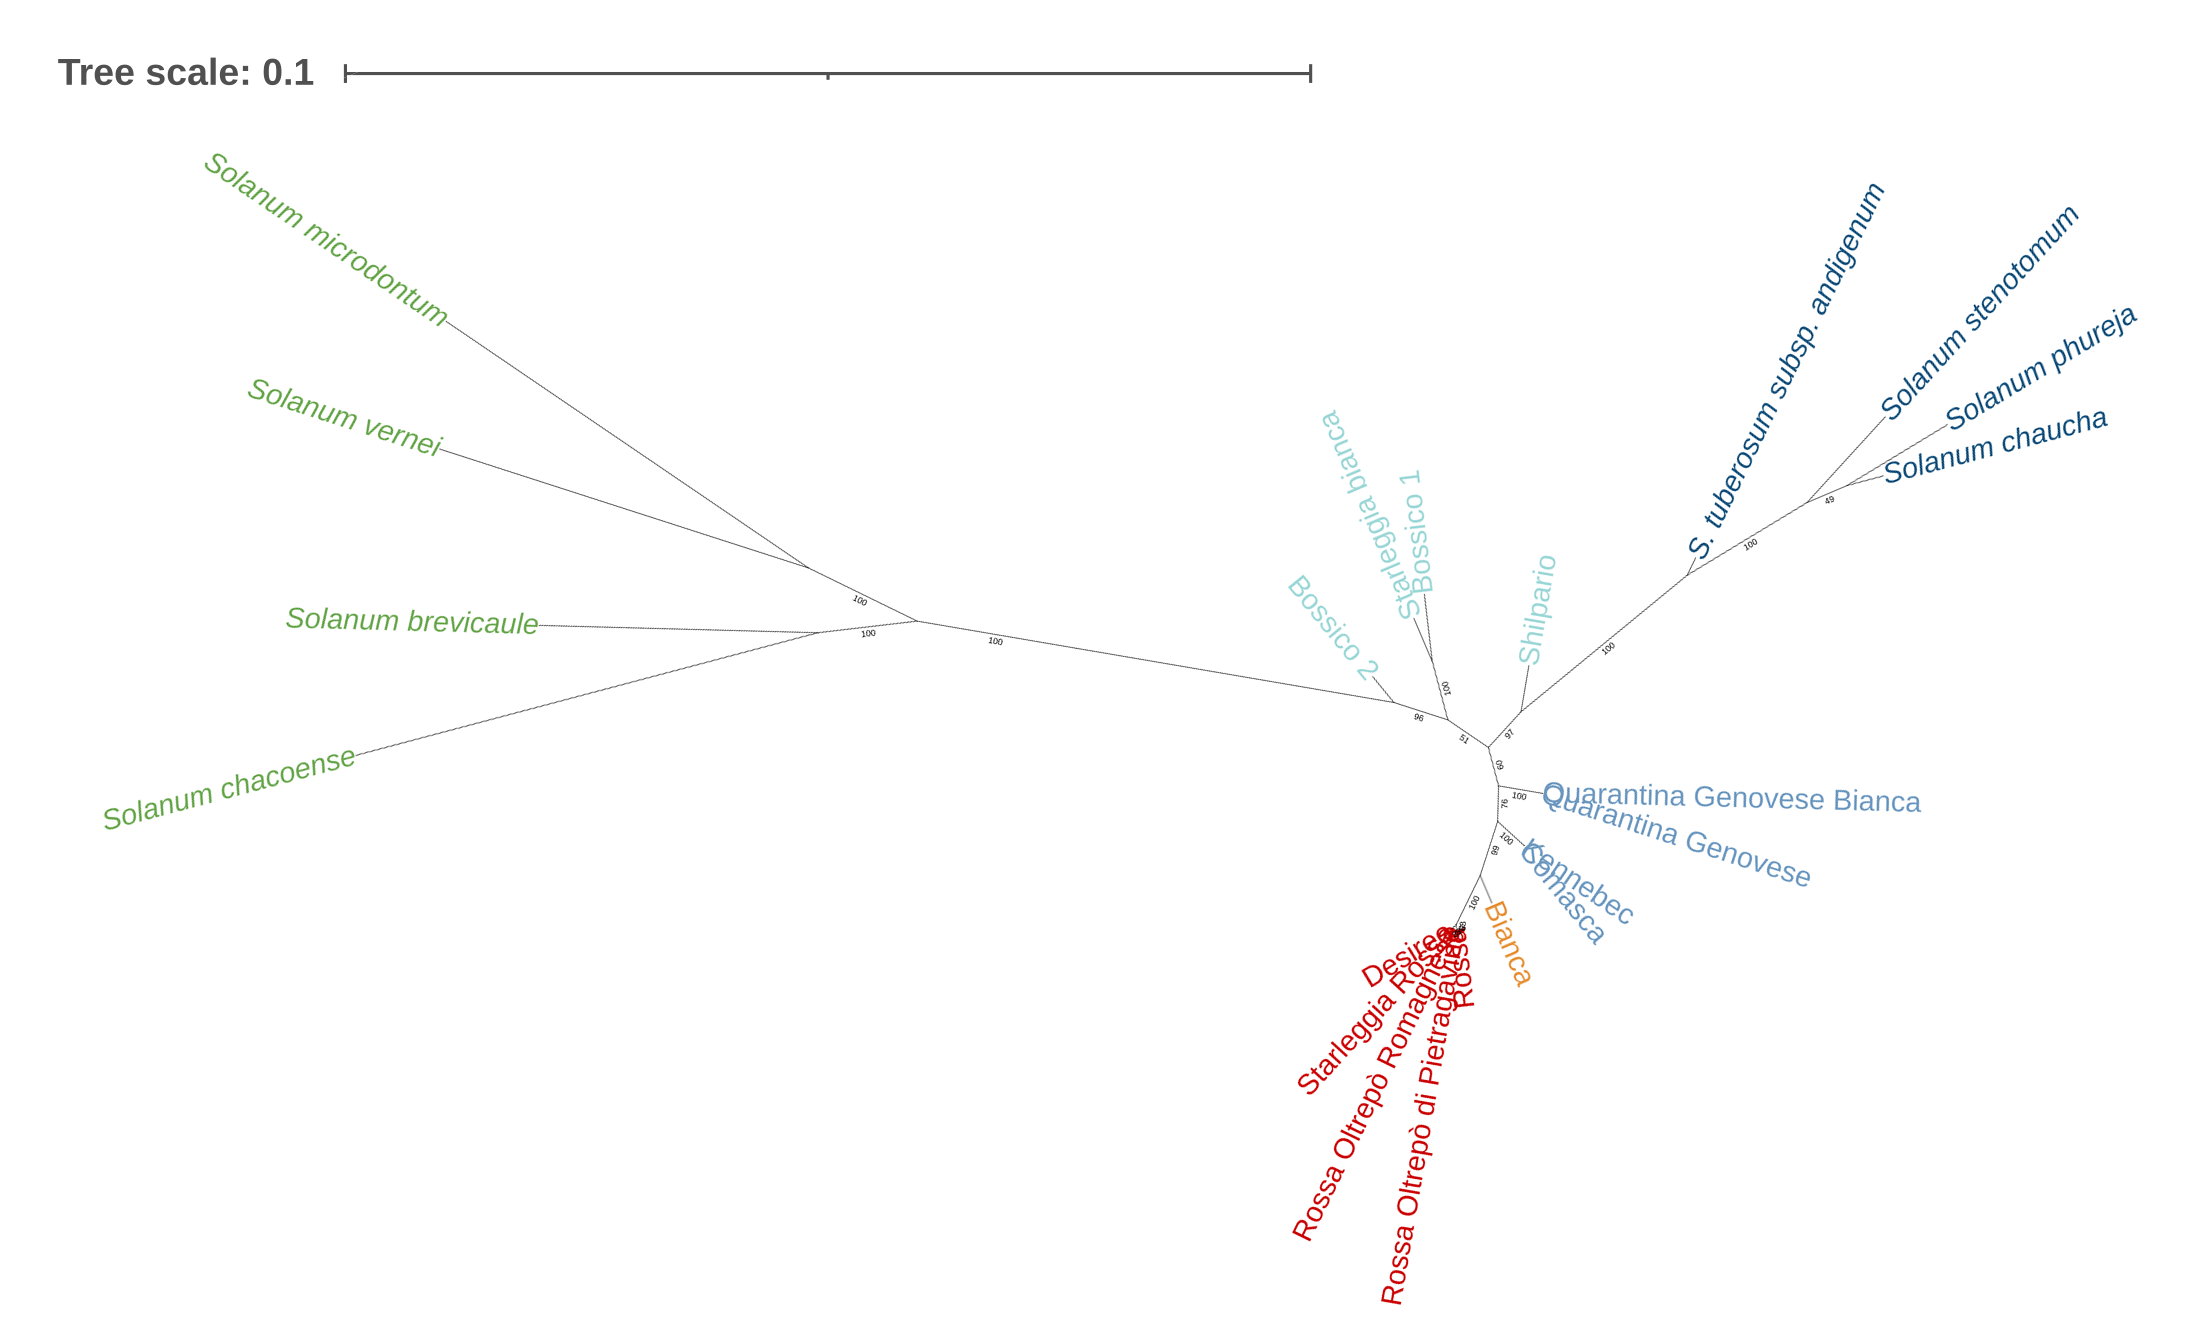
\includegraphics[width=1\textwidth]{unrooted_ML_tree_potatoes2.png}
	\caption{\justifying{\footnotesize \textit{\textbf{Unrooted maximum likelihood tree of \textit{Solanum} genus and landraces.} \footnotesize{Phylogenetic maximum likelihood (consensus) tree.}}}}
	\label{fig:unroteed_patate}
\end{figure}

Although, from now on, we are going to comment the rooted tree in Figure \ref{fig:albero_patate} because of its clearer visualization, the results are the same as in the unrooted tree (Fig. \ref{fig:unroteed_patate}), with the addition of a putative root of the tree set on the wild species clade. On the topic of evolutionary history between the samples, the tree shows, with high bootstrap support, that Bossico 2 ($bootstrap = 96$), Bossico 1 and the cultivar Starleggia Bianca (together $bootstrap = 100$), are the ones closer to the wild species (i.e. \textit{S. vernei}, etc...), and not, as we would expect, the Andean cultivated ones (i.e. \textit{S. stenotomum}, etc...). Bossico 1, Bossico 2 and Starleggia Bianca are still phylogenetically closer to the Andean cultivated species. With an equally high support ($bootstrap = 97$), the obsolete landrace Shilpario from the Botanical Garden of Bergamo, is shown to have separated from the cultivated Andean species even before the commercial variants Kennebec and Desiree. These evolutionary relationships between cultivated Andean species and the landraces is what was caught by PC2 in the PCA plots (Fig. \ref{fig:pca_patate}, b and c), and which we highlighted as old/recent divergence. All the red-peel cultivars cluster very closely together with $bootstrap = 100$ and very short branches length. Furthermore, the internal branches of this clade have low boostrap support; for example, Rossa Oltrepò Romagnese, Starleggia Rossa and Desiree separate from the other two red peel variants with a weak bootstrap support of 59, and the situation is similar for the other landraces in this group. This information let us to believe that red peel landraces are, in fact, not old Italian landraces but clones or cultivars closely related to the commercial variant Desiree.

 \begin{figure}[h!]
	\centering
	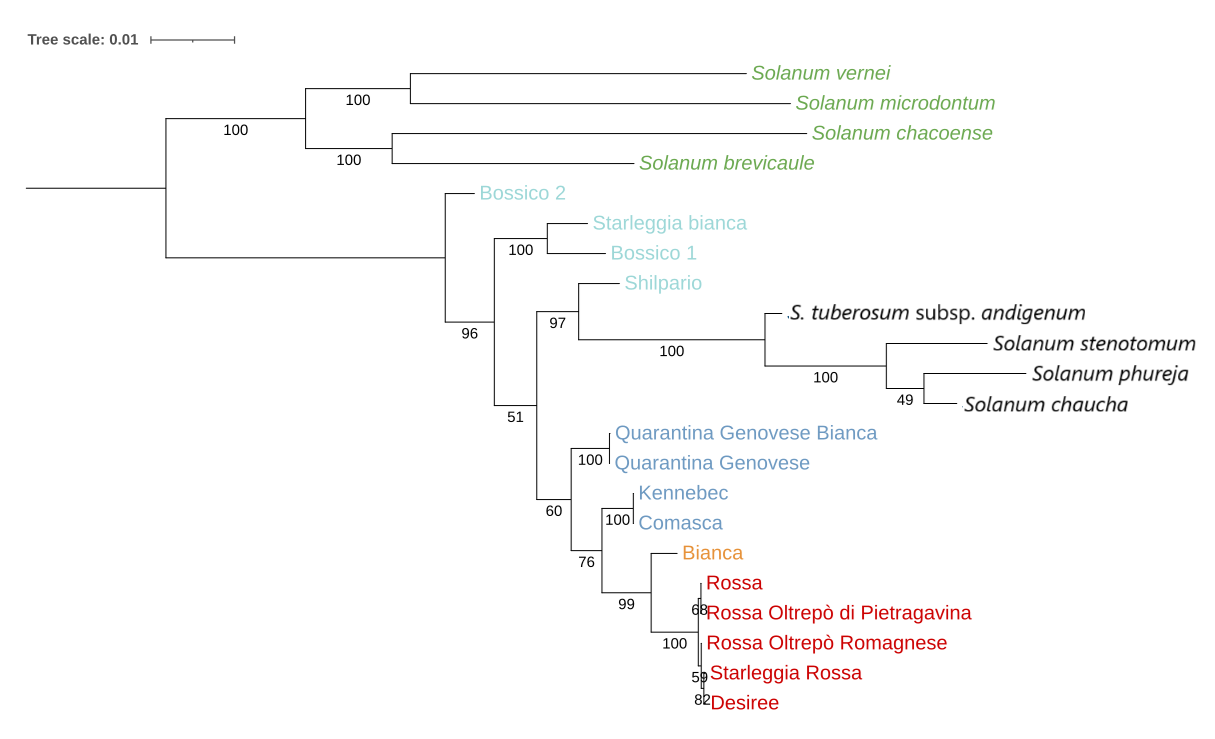
\includegraphics[width=1\textwidth]{rooted_ML_tree_potatoes.png}
	\caption{\justifying{\footnotesize \textit{\textbf{Rooted maximum likelihood tree of \textit{Solanum} genus and landraces.} \footnotesize{Phylogenetic maximum likelihood (consensus) tree rooted on the most distant clade comprised of wild species. Tips colors reflect those in the PCA plot (Fig. \ref{fig:pca_patate}).}}}}
	\label{fig:albero_patate}
\end{figure}

The situation is more complicated when observing white peel variants: they do not cluster as close together as the red peel potatoes did in both PCA plots (Fig. \ref{fig:pca_patate}) and in the phylogenetic trees (Fig. \ref{fig:unroteed_patate} and \ref{fig:albero_patate}). Landrace Bianca is located halfway through white and red peel variants with a high support ($bootstrap = 99$) , suggesting being the result of hybridization between red and and white peel cultivars. All the remaining landraces, even if all belonging to the same white peel category, do not cluster in the same clade: we can confirm that Kennebec is more similar to Comasca and the two Quarantina group together (both $bootstrap = 100$), but we concluded that these two are close relatives of the commercial cultivar Kennebec since their division in two different groups is not well supported ($bootstrap = 60$). As mentioned before, the remaining 4 landraces (Bossico 1 and 2, Starleggia Bianca and Shilpario) can not be as easily included in this cluster. Bossico 1, Bossico 2 and Starleggia Bianca were described before, and we can confidently say they are well separated from all the other cultivated species, both Andean and Italian white and red peel variants. When, instead, we consider Shilpario and the group of cultivated Andean species, the division of them from the commercial cultivars is not well supported ($bootstrap = 51$), which is in line with them being all (minus Shilpario) currently cultivated. When the branches diverge, though, the landrace Shilpario groups with the Andean species with high support ($boostrap = 97$), and this is the reason why we did not include it with the other commercial cultivars/landraces, and we suspected that it is the result of an older divergence from \textit{S. tuberosum}.

\clearpage
\section{\textit{Anacamptis} spp.}
After we tested all of the software for $F_{ST}$ estimation on \textit{Campanula} dataset, we used \textit{Anacamptis} to compare the first software used (\texttt{populations}) against the one we chose as optimal (\texttt{StAMPP}). 


\clearpage
\chapter{Discussion}

\section{\textit{Campanula thyrsoides}}
Choosing the appropriate restriction enzyme in GBS is important because of the absence of a size selection step \parencite{sonahImprovedGenotypingSequencing2013}: our samples still showed satisfactory quality after PCR amplification, but the fact that we improved the proportion of reads of the correct length using a size selection kit (refer to the Materials and Methods section) shows that a proper \textit{C. thyrsoides} GBS protocol needs to be further investigated. In soybeans ApeKI has proven to be the most appropriate choice in comparison to enzymes like PstI, MseI and MspI \parencite{sonahImprovedGenotypingSequencing2013}, but the two species differ in number of chromosomes (12 for \textit{C. thyrsoides} and 20 for soybean) and genome size (putative 4.83Gb for \textit{C. thyroides} and 978.4 Mb for soybean\footnote{Following v2 of the assembly, NCBI RefSeq assembly GCF\_000004515.4.}), which can influence the restriction enzyme efficacy. Furthermore, the choice of enzyme can largely benefit from the use of a reference genome \parencite{sonahImprovedGenotypingSequencing2013},  not availablewhich is a limitation in our study and should be addressed in the 


The definition of specialist species is debated, but following \citeauthor{kirschDefiningPlantEcological2022} (\citeyear{kirschDefiningPlantEcological2022}), we could define \textit{C. thyrsoides} subspecies \textit{carniolica} as ambiguously specialized: it has a restricted range in habitat diversity \parencite{aegisdottirIsolatedPopulationsRare2009} like a specialized species but doesn't present highly modified anatomy \parencite{scheepensDifferentiationMorphologyFlowering2011} or high reliance on interspecies interactions, aside from its pollination through bumblebees \parencite{kussBiologicalFloraCentral2007}. Specialist species with lower dispersal (as in the case of \textit{C. thyrsoides}; \cite{aegisdottirIsolatedPopulationsRare2009}) usually have isolated population that can lead to a strong genetic differentiation among populations but also less genetic diversity within them due to small population sizes \parencite{hughesStrongGeneticStructuring1999}. Populations of subspecies \textit{carniolica}, small and isolated at medium-high altitudes, have low nucleotide diversity ($\pi$\footnote{Defined as the average sequence divergence between any two individuals for a given locus \parencite{bucklerPlantMolecularDiversity2002}.}) and moderate differentiation ($F_{ST}$), as expected from a species with limited dispersal \parencite{hughesStrongGeneticStructuring1999}, but they also show extremely low inbreeding factors ($F_{IS}$). This confirms the presence of a good genetic flow that was already found in the subspecies \textit{thyrsoides} despite its limited seed dispersal capacity \parencite{aegisdottirIsolatedPopulationsRare2009}. Subspecies \textit{carniolica} might even have an advantage in this sense, since a taller inflorescence may cause a farther seed dispersal \parencite{scheepensDifferentiationMorphologyFlowering2011}. Small populations size can be caused by both recent loss of habitat \parencite{yinPlantConservationAge2024} and its monocarpic characteristic, but the latetr might be also the reason why \textit{C. thyrsoides} subspecies \textit{carniolica} populations show no inbreeding depression: genetic erosion is usually more pronounced after several generation \parencite{aguilarGeneticConsequencesHabitat2008}, so by reproducing once in their life, the risk for individuals of this species is mitigated. This adaptation to an habitat that forces fragmentation due to its geography \parencite{aegisdottirNoInbreedingDepression2007} can be an additional sign of \textit{C. thyrsoides} subspecies \textit{carniolica} specialist nature. Common gardens experiments are frequently used to test for habitat adaptation ((TROVARE CITAZIONE)): 



No population is in need of immediate intervention: the low nucleotide diversity ($\pi$) with a high within ($F_{IS}$) and between ($F_{ST}$) populations diversity is expected from a specialized species \parencite{habelBurdenGeneticDiversity2012}, so we would conclude that \textit{C. thyrsoides} subspecies \textit{carniolica} is moderately specialized. It could be caused by the combined effect of two \textit{C. thyrsoides} characteristic. Its ability to mate with its half-siblings \parencite{aegisdottirNoInbreedingDepression2007} raises its high differentiation among populations like a selfing species but being an outcrossing species \parencite{aegisdottirIsolatedPopulationsRare2009}, it also possesses large within-population diversity \parencite{aguilarGeneticConsequencesHabitat2008}. As an open-pollinated, outcrossing and self-incompatible species, \textit{C. thyrsoides} could've suffered from outbreeding depression\footnote{Defined as reduction of fitness after hybridization events \parencite{volisQuasiSituBridge2010}.} \parencite{volisQuasiSituBridge2010}, but hybrids of subspecies \textit{carniolica} and \textit{thyrsoides} are currently not documented. Due to the limited number of samples in the outgroup CTT we cannot say if the same conclusion applied to the whole subspecies \textit{thyrsoides} too, but it appears to apply to the population in our study.

\subsubsection{Pian dei Resinelli}
Historically speaking, the region of Lombardia (Italy) had only shown sights of the subspecies \textit{thyrsoides} but the top PCA plots clearly cluster the population of PDR (Pian dei Resinelli, Lombardia) with the other populations of subspecies \textit{carniolica}, with PC3 (Fig. \ref{fig:PCA}, b) clearly catching this separation. When the outgroup CTT of subspecies \textit{thyrsoides} is included in the analysis, PDR clearly separates from it, but when CTT is excluded (Fig. \ref{fig:PCA}, d, e and f), PDR separates from the other populations of subsp. \textit{carniolica}, showing its own distinct pool of genetic information. This shows an expansion in its historical habitat: this highlights the need of a new census to update the last one, done in 2005 \parencite{fabiocontiAnnotatedChecklistItalian2005}.  

\subsubsection{Slovenian populations}
Slovenian populations (RT and STE) group together very well: it was previously observed that in the lower mountains of Slovenia, subspecies \textit{carniolica} showed a later (in comparison to \textit{thyrsoides}) end of flowering \parencite{scheepensDifferentiationMorphologyFlowering2011}. A longer flowering period of those populations fits well with the phenology of alpine species in warmer climate, which already demonstrated, in other species, the same behavior when subject to shift in snowmelt dates \parencite{vorkaufFloweringPhenologyAlpine2021}. Following the hypothesis that Slovenian populations might be more adapted to the climate and drought \parencite{scheepensDifferentiationMorphologyFlowering2011}, we integrated their low sampling altitude (245m - 420m) with their clear clustering in the PCA and concluded that our analysis might have caught some of the genetic information linked to the adjustment to their habitat.  The reduced sequencing approach, though, can not confirm if these populations are generally more adapted to their habitat: higher adaptation is usually accompanied by lower genetic variety \parencite{habelBurdenGeneticDiversity2012}, but RT and STE $\pi$ levels are not lower than the rest of \textit{carniolica} populations, nor their $F_{IS}$ values largely higher. Confirmation of this adaptation hypothesis requires a more detailed study, combining drafting of a reference genome and annotation of genes, to connect genomic regions to traits, which can lead to conservation plans for populations carrying them \parencite{suppleConservationBiodiversityGenomics2018}.

\subsubsection{Alpago (ALP)}

It is good practice to choose a genetically close population when planning a translocation intervention in order to minimize outbreeding depression risk \parencite{yinPlantConservationAge2024}. ALP is the closest population to SP using weighted $F_{ST}$ estimates and its individuals could be translocated to Monte Serva, but they show admixture (Fig. \ref{fig:structure}), which is usually caused by breeding of individuals belonging to two distinct groups \parencite{suppleConservationBiodiversityGenomics2018}. Alpago (ALP) shows shared ancestry with the populations from the Veneto-Friuli group (Fig. \ref{fig:structure}, cluster 1), but its admixing probably comes from another population too, potentially not included in our samples. With its admixed structure, ALP has the potential of acting as a source of new genetic variation \parencite{suppleConservationBiodiversityGenomics2018},which could be either positive or negative. Potentially deleterious alleles should be identified before trans-locating its individuals to another population and, since the target population of Monte Serva does not currently show breeding depression (its $F_{IS} < 0$), the risks outweigh the benefits.

\subsubsection{Outgroup \textit{thyrsoides} (CTT)}
$F_{IS}$ value seems to be slightly lower for population CTT (subspecies \textit{thyrsoides}, Table \ref{tab:fis}). We could hypothesize that subspecies \textit{thyrsoides}, which is more common, is less specialized than subspecies \textit{carniolica}: the lower level of specialization can explain an higher level of gene flow \parencite{habelBurdenGeneticDiversity2012}, thus lower $F_{IS}$. But, because of the low number of samples in the outgroup CTT, we can not statistically test whether it depends on its belonging to subspecies \textit{thyrsoides} or if it is a limited case in this specific population. We also suspect that the two subspecies might be actually on the early stages of a speciation event as they're relatively isolated from one another \parencite{hughesStrongGeneticStructuring1999}, following their post-glacial allopatric subspeciation event with no secondary contact \parencite{kussSpatialGeneticStructure2011}. To be able to confirm this theory, a new study with a different research question than ours, should be planned: up until now, comparative studies between subspecies \textit{thyrsoides} and \textit{carniolica} have only focused on morphological differences \parencite{scheepensDifferentiationMorphologyFlowering2011} and flowering behavior \parencite{kussSpatialGeneticStructure2011}, while a genetic study on population structure has been carried only on subspecies \textit{thyrsoides} \parencite{aegisdottirIsolatedPopulationsRare2009}. A comparative analysis between the two subspecies structure, increasing the number of populations and individuals sampled for both, could shed more light on their evolutionary relationship and whether or not they are currently affected by early stages of divergence. This diverging pressure can be intense due to the small populations size \parencite{hughesStrongGeneticStructuring1999}, but to encourage this process it is important to keep the two subpopulations separated from one another as they have been until now.

\clearpage
\section{{\textit{Solanum tuberosum} landraces}}
In our study GBS was able to capture many interesting evolutionary relationships in the set of potatoes of genus \textit{Solanum} we selected: we contextualize now our findings to give more insights on the necessity of local landraces conservation. 

\subsection{Wild and ancient species}
Wild species were correctly assessed as the most genetically distant samples, both in the PCA and phylogenetic trees: they cluster together as they are all wild, but in the tree (Fig. \ref{fig:albero_patate}) they present very long branches, highlighting the large genetic difference even between them. This was expected since they are not currently used as a food source, so they are rarely cross-bred. On the other hand, all the Andean cultivated species easily cluster together with branches of shorter length, probably because when using different taxonomies \textit{S. chaucha}, \textit{S. phureja} and \textit{S. stenotomum} are actually considered cultivars of \textit{S. tuberosum} \parencite{machida-hiranoDiversityPotatoGenetic2015}. In some studies they are considered even hybrids: in \citeauthor{huamanReclassificationLandracePopulations2002} (\citeyear{huamanReclassificationLandracePopulations2002}), \textit{S. chaucha} is reported to probably be an hybrid of \textit{S. tuberosum} subsp. \textit{andigenum} with either \textit{S. stenotomum} or \textit{S. phureja}, with the latter being a divergence of the former. This is probably why these three species are separated from \textit{S. tuberosum} subsp. \textit{andigenum} with high bootstrap support (100), but the relationships between them are not well captured by a tree ($boostrap = 49$) between them. Nevertheless, this further proves how interesting is that Bossico 1, Bossico 2 and Starleggia bianca separate so clearly from this group, raising their importance in conservation plans as landraces largely different from modern cultivars of \textit{S. tuberosum}.

\subsection{Italian landraces}
Quarantina genovese is one of the landraces that is currently conserved \textit{ex-situ}, specifically by the "Consortium for the protection of the Genoese white Quarantina and the traditional potatoes of the Genoese mountain" (http://
www.quarantina.it/category/il-consorzio/), recognised by the International Treaty on Plant Genetic Resources for Food and Agricolture (ITPGRFA). Our findings, though, collocated this type of potato genetically close to the commercial variant Kennebec. The clustering of the two landraces with each other is evident in both the PCA plots (Fig. \ref{fig:pca_patate}) and in the phylogenetic tree (Fig. \ref{fig:albero_patate}) where their clade showed a perfect bootstrap support (100): from these results, we could suspect a strong genetic identity of this landrace. Recent studies on Italian local landraces of \textit{S. tuberosum} have, though, shown significant similarity of Quarantina Genovese Bianca with commercial variant Kennebec both morphologically \parencite{giupponiMorphometricPhytochemicalCharacterization2020} and genetically \parencite{martinaConservationValorizationItalian2025}. In the study by \citeauthor{martinaConservationValorizationItalian2025} (\citeyear{martinaConservationValorizationItalian2025}), Quarantina also belonged to a sub-cluster containing a French white peel commercial cultivar (Institute de Beauvais). Although this commercial cultivar was shown to be genetically identical to Quarantina Genovese Bianca using microsatellites markers \parencite{mandolinoMOLECULARFINGERPRINTINGTRADITIONAL2015}, GBS analysis on the same species, with its enhanced resolution, caught a certain degree of differentiation \parencite{martinaConservationValorizationItalian2025}. We concluded that, although our two Quarantina landraces show good clustering within themselves, they are too similar to commercial variants in our studies as well in others, so we could not consider them a genetically distinct variety. This might be different for other Quarantina landraces not object of our study (i.e. Quarantina Prugnona and Ruba Spes, a red peel mutation of Quarantina Bianca), that already showed differences from Kennebec in morphology \parencite{giupponiMorphometricPhytochemicalCharacterization2020}, so we would not exclude from conservation efforts the Quarantina landrace in its entirety.

The case of Comasca (CO) overlapping with Kennebec instead, seems to be a simple mix-up. In the area of Como, many old cultivars have been replaced by the dutch commercial variety Kennebec: for example, the name "Patata di Martinengo" is currently applied to local production of Kennebec \parencite{rossiVarietaAgronomicheLombarde2019}. The same thing was happening until a couple of years ago to other cultivars: both names "Patata bianca di Oreno" and "Patata bianca di Rovetto", were used to actually refer to the aforementioned commercial variant. Years ago, the name "Patata bianca di Rovetto" was also used to refer to "Bianca di Como" \parencite{rossiVarietaAgronomicheLombarde2019}, Italian for "White peel variety of Como", which is nowadays used as a synonym of  "Comasca". It is therefore likely that the seeds we were given as "Comasca" were mistakenly believed to be the local landrace "Bianca di Como" that in 2007 has been promoted as local potato cultivation in the Brianza, by the municipality of Vimercate. And, instead, they were probably the old "Bianca di Como", that was in fact a "Patata bianca di Rovetto", which was simply another name for a Kennebec cultivar in Como.

Both Starleggia Bianca and Rossa were reported as local landaraces of Campodolcino (SO) \parencite{rossiVarietaAgronomicheLombarde2019} and currently cultivated as such \parencite{veginiPatateTradizionaliLocali2022}. Our study, instead, highlighted the genetic differentiation of only Starleggia Bianca, the white peel variant, while Starleggia Rossa (red peel) vastly overlaps with all the other red peel varieties. These varieties are genetically indistinguishable from each other in our tree (Fig. \ref{fig:albero_patate}) and it probably is caused by potatoes being bred by cloning. This technique allows to artificially select desiderable traits and since \textit{S. tuberosum} is, originally, a white peel potato, the red peel phenotype had to be artificially selected and bred. The uniformity of these samples should raise concerns due to the inevitable genetic erosion and vulnerability that these cultivars might suffer from \parencite{salgotraGeneticDiversityConservation2023}. The genetic difference between Starleggia Rossa and Starleggia Bianca was already suspected due to the already observed morphological differences \parencite{rossiVarietaAgronomicheLombarde2019}: while we categorized Starleggia Rossa as a clone of a commercial variant, our study is limited due to small sampling. Repeating this type of genetic study on a larger set of samples could refute this conclusion, and thus either promote or discourage conservation of this variety in seed banks.

Our analysis confirmed that "Rossa Oltrepò di Pietragavina" is a clone of the Dutch commercial cultivar Desiree, already suspected due to many similarities in their morphological characteristics \parencite{rossiVarietaAgronomicheLombarde2019}.

Lastly, the intermediate position of landrace Bianca between white and red peel variants in both the PCA and phylogenetic tree, shows that it might be an hybrid, probably the result of cross-breeding between white and red commercial cultivars. This highlights the power of GBS in catching even the smallest nuances of genetic diversity and phylogenetic relationships.


\clearpage
\section{\textit{Anacamptis} spp.}
\vspace{-1.5em}
Separation of species, not of populations
Cannot differentiate between natural and urban, while instead species are very divided: this shows that the pipeline is robust in also underline similarities and do not force subdivisions if they aren't supported.


\clearpage
\chapter{Conclusion and future perspectives}
Monitoring of genetic erosion and biodiversity vulnerability should be a top priority in the protection of plant species \parencite{salgotraGeneticDiversityConservation2023}: the GBS approach used in this study shows robustness to different non-model organisms, performing exceptionally well both in the presence or not of a reference genome and with the use of different types of restriction enzymes. These are good news for laboratories looking to contain costs but of course interested in delivering high quality results and studies. The same steps could be applied with different kingdoms, namely Animal and Fungi. Archea and Bacteria could benefit from this approach but its not strictly necessary, due to the incredibly smaller genome they possess. 

\section{\textit{C. thyrsoides} subspecies}
Populations of subspecies \textit{carniolica} are not endangered, but the small number of individuals (probably caused by it being monocarpic; \cite{aegisdottirIsolatedPopulationsRare2009}) requires conservation actions of their habitat. Although highly specialized species can thrive in isolated population networks, the loss of habitat because of industrial agriculture needs to be limited since these networks need to be intact to ensure survival \parencite{habelBurdenGeneticDiversity2012}. It is also unknown if the two subspecies of \textit{C. thyrsoides} are interfertile and produce viable offsprings \parencite{scheepensDifferentiationMorphologyFlowering2011}: now that subspecies \textit{carniolica} seems to be moving towards the habitat of subspecies \textit{thyrsoides}, it is crucial that their differences are highlighted and preserved. Since habitat preservation is the top priority in the case of a moderately specialist species \parencite{habelBurdenGeneticDiversity2012}, the National Park of Dolomiti Bellunesi is already correctly applying the \textit{in situ} technique of the genetic reserve conservation area \parencite{salgotraGeneticDiversityConservation2023}, by protecting in its territory Monte Serva population (SP). \textit{C. thyrsoides} habitat needs to be preserved, in particular, from further fragmentation due to the usage of alpine regions as summer pasture for cattle \parencite{freiHighGeneticDifferentiation2012}. The park also committed to increase Monte Serva population's size by either breeding \textit{ex-situ} individuals of its population and reintegrating them in the habitat, or by genetic rescue, meaning translocating individuals from the closest populations \parencite{suppleConservationBiodiversityGenomics2018} Alpago (ALP) and Passo del Pura (PPURA). We would prioritize PPURA as one of the closest populations to SP currently not experiencing high level of admixing, like ALP, that could introduce deleterious genetic variance. In fact, since the intervention is going to be carried on after a genetic study, also ensures that the park's intervention won't disrupt Monte Serva's ancestry, so we recommend other parks and institutions to follow a similar approach. An analogous analysis should be repeated in a couple of years after the park's intervention to correctly quantify the efficacy and future potential of both these analysis and the conservation efforts. Furthermore, despite parks and other associations' best efforts, because of climate change the potential of \textit{in situ} preservation for the persistence of species in the wild is declining \parencite{iucn/sscGuidelinesUseEx2014}, raising our concerns about subspecies \textit{thyrsoides} too. Subsp. \textit{carniolica}, being slightly more specialized on lower altitudes and so higher temperatures, could be invading \textit{thyrsoides} habitat due to the increase of temperature. Even if the latest genome-editing technologies might allow researches to improve species traits to adapt to the changing climate (\cite{suppleConservationBiodiversityGenomics2018}; \cite{yinPlantConservationAge2024}), we instead need to intervene on preservation of the habitat on a larger scale, which includes taking action on mitigating our impact on the Earth.

\section{\textit{S. tuberosum} local landraces}
Since the lack of genetic screening before any kind of intervention in a breeding program is discouraged for crop plants too because it can lead to unexpected epidemic of diseases \parencite{salgotraGeneticDiversityConservation2023}, Project Rava la Fava for \textit{S. tuberosum} landraces conservation correctly asked for a genetic study when choosing which landraces focus their effort on. In our analysis on genus \textit{Solanum}, we combined Italian and South American accessions, managing to highlight a distinct phylogenetic identity for some of the local landraces in this study. To limit the loss of genetic diversity for \textit{S. tuberosum} in our national territory, it might be useful to include currently obsolete cultivars (Bossico and Shilpario; \cite{veginiPatateTradizionaliLocali2022}) to plant genetic resources (PGRs) collections, an \textit{ex-situ} conservation method started in the mid-20th century, that aims at gathering all cultivated, wild relatives, traditional cultivars, landraces, and advanced breeding lines of plants \parencite{salgotraGeneticDiversityConservation2023}. Other studies highlighted the need to prioritize local germplasm, underutilized crop species and traditionally local landraces \parencite{salgotraGeneticDiversityConservation2023}: considering the benefits that can result from conserving locally adapted landraces, we stress the importance of centering the efforts on Bossico and Shilpario. PGRs collections could benefit also from the addition of Starleggia Bianca, although it is already currently cultivated for conservation purposes by different societies like Mato Grosso Association and Legambiente Valchiavenna \parencite{veginiPatateTradizionaliLocali2022} so a conservation intervention is less urgent. In 2004, the Italian Ministry of Agriculture, Food Sovereignty and Forests (MiPAAF), following the International Treaty on Plant Genetic Resources for Food and Agriculture (ITPGRFA), financed the project RGV/FAO for the realization of the objectives in the Treaty: to do this, in 2013 it included around 17,000 accessions across 22 genus of plant genetic resources in the Multilateral System of Access and Benefit-sharing \parencite{ammassariNotificationRegardingContribution2013}. Its germplasm databanks are available at PlantaRes database (Network Nazionale delle Risorse Genetiche Vegetali per l'Alimentazione e l'Agricoltura) and at the Mediterranean Germplasm Database (MGD). Currently (September 2025), the MGD doesn't include any accession to \textit{S. tuberosum}, and even so, it only provides germplasm exclusively as a support to research and education projects and not for crop improvement\footnote{Information MGD Policy can be found at web address: https://www.ibbr.cnr.it/mgd/?action=page\&id=policy.}. PlantaRes database, instead, contains information about two landraces of \textit{S. tuberosum} (Accession names Montecopiolo and Patata Blu), whose germplasm is currently stored at the Horticulture and Floriculture Center of Monsampolo del Tronto (AP). There is another center associated with CREA, at Bergamo (Cereal and Industrial Crop Research Center - Bergamo branch), so storing Bossico 1, Bossico 2, Starleggia Bianca and Shilpario seeds there can be a proper additional \textit{ex situ} approach for the conservation of these local landraces, in line with both RAVA la FAVA and ITPGRFA projects.

\clearpage
\chapter{Bibliography}
\printbibliography

\clearpage
\chapter{Additional material}\label{chap:additionalmaterial}
Here are listed and reported all the materials named and used for the preparation and analysis of data for \textit{Campanula thyrsoides}: for the sake of being concise, we avoided going in detail in chapter \ref{Materials and Methods}. Materials and Methods. All information is reported here and, in the case of pipelines and additional files, is freely downloadable from the Github repository \texttt{flavialeotta /Master-thesis}.
\vspace{-1em}
\section{Protocols}
\vspace{-1em}
In this section are reported, in detail, the protocols used in the wet lab before receiving the data: they can give some insight on how the samples were prepared and treated, which can influence the quality of data, as previously discussed.
\vspace{-1em}
\subsection{SILEX: CTAB-Silica extraction protocol}
\vspace{-1em}
SILEX is a highly-throughput DNA extraction protocol, based on the standard CTAB method with a DNA silica matrix recovery. Here we report the steps taken to extract the DNA samples needed to produce the NGS data used in the previous analyses. \parencite{vilanovaSILEXFastInexpensive2020}
\vspace{-1em}
\begin{enumerate}\setlength\itemsep{-0.2em}
\item Grind the tissue with Qiagen TissueLyser;
\item Add 1 mL of CTAB extraction buffer and 14 mL of $\beta$-mercaptoethanol for each sample and vortex, until complete homogenization;
\item Incubate in a thermoblock at 65°C for 45 minutes;
\item Let the samples rest on ice for 5 minutes;
\item Add 700 $\mu$L of the protein precipitation buffer, which is a solution of Chloroform:Isoamyl Alcohol (24:1), and turn the tubes upside down to mix the solution;
\item Centrifuge at 11000 rpm for 5 minutes;
\item Transfer 800 $\mu$L of supernatant phase in a new 2 mL tube;
\item Add 2,5 $\mu$L of RNAse and incubate at 35°C for 20 minutes;
\item Add 480 $\mu$L of binding buffer (25M NaCl + 20\% PEG 8000) and gently invert the tube by hand to mix the solution;
\item Add 700 $\mu$L of EtOH 100\% and turn the tubes upside down;
\item Add 20 $\mu$L of silica matrix buffer\footnote{The Silica matrix buffer must be prepared beforehand following the protocol by Vilanova \textit{et al.} \parencite{vilanovaSILEXFastInexpensive2020}.} and shake for 5 minutes;
\item Centrifuge for a few seconds and discard the supernatant;
\item Add 700 $\mu$L of EtOH 70\%;
\item Suspend silica by turning the tubes upside down and spin again for a few seconds;
\item Discard the supernatant and turn the tubes upside down on paper for 10 minutes to let ethanol fully evaporate;
\item Add 100 $\mu$L elution buffer (10 mM Tris HCl pH 8.0 and 1 mM EDTA pH 8.0) and shake gently by hand until the pellet is re-suspended;
\item Incubate at 65°C for 3-5 minutes;
\item Centrifuge at 14000 rpm for 10 minutes;
\item Pipette 70 $\mu$L of supernatant and store it in a 1.5 mL Eppendorf.
\end{enumerate}

\subsection{DNA digestion}
\vspace{-1em}
DNA digestion protocol was used to digest the same quantity of DNA for each sample. Since the goal was to digest 50 ng of DNA and each sample had a different concentration, we calculated the volume of DNA to digest for each sample \textit{i} as:
\begin{equation}\label{volDNA} 
	V_{DNA_i} = \frac{m \ (ng)}{[DNA]_{i} \ (ng / \mu L)}= \frac{50 \ ng}{[DNA]_{i} \ (ng/\mu L)}
\end{equation}
by using the concentration of DNA as obtained using Qubit. The samples to digest ($50 \mu L$ each), to be prepared on ice, had to contain:
\vspace{-1.5em}
\begin{enumerate}\setlength\itemsep{-0.2em}
	\item first distilled and de-ionized water ($ddH_2O$) calculated as $44 \mu L - V_{DNA}$ and reported in Table \ref{tab:digestion};
    \item then $4\mu L$ of NEBuffer\textsuperscript{TM} r3.1 10x; \footnote{1X NEBuffer\textsuperscript{TM} r3.1 contains: 100 mM NaCl, 50 mM Tris-HCl, 10 mM MgCl2, 100 µg/ml Recombinant Albumin (pH 7.9 @ 25°C).}
    \item extracted DNA as calculated with formula \ref{volDNA} and reported in Table \ref{tab:digestion};
    \item $2 \mu L$ of ApeKI $(\frac{5U}{\mu L})$. \footnote{U stands for enzyme unit, and is related to the katal by the following: $1 \ U = 16.67 \ nkat$. \parencite{nomenclaturecommitteeoftheinternationalunionofbiochemistrync-iubUnitsEnzymeActivity1979}. We know that the catalytic activity of an enzyme is the increase in the rate of chemical reaction that the enzyme produces. The katal (symbol: kat) is that catalytic activity, that will raise the rate of reaction’ by one mole per second.}
\end{enumerate}
\vspace{-1.5em}
The samples went through four different protocols for digestion (Table \ref{tab:digestion}): the difference between them are minimal. Those that got digested for 4 hours and then incubated in a thermocycler (80°C lid, hold 20°C) for an additional 8 hours with more ApeKI and buffer, show better smears in digestion but only slightly better bands in amplification.

\begin{table}[h!]
	\centering
	\caption{\textit{Digestion information}}
	\label{tab:digestion}
	\resizebox{\textwidth}{!}{
		\begin{tabular}{|>{\centering\arraybackslash}p{2.2cm} |
				>{\centering\arraybackslash}p{1.5cm} |
				>{\centering\arraybackslash}p{1.5cm} |
				>{\centering\arraybackslash}p{1.5cm} ||
				>{\centering\arraybackslash}p{2.2cm} |
				>{\centering\arraybackslash}p{1.5cm} |
				>{\centering\arraybackslash}p{1.5cm} |
				>{\centering\arraybackslash}p{1.5cm} ||
				>{\centering\arraybackslash}p{2.2cm} |
				>{\centering\arraybackslash}p{1.5cm}|
				>{\centering\arraybackslash}p{1.5cm}|
				>{\centering\arraybackslash}p{1.5cm}|}
			\toprule
			\textbf{Sample ID} &\textbf{$ng/\mu L$ qubit} & \textbf{$\mu L$ sample} &$\mu L$ $H_2O$ &\textbf{Sample ID} & \textbf{$ng/\mu L$ qubit} & \textbf{$\mu L$ sample} & $\mu L$ $H_2O$&\textbf{Sample ID} & \textbf{$ng/\mu L$  qubit} & \textbf{$\mu L$ sample} & $\mu L$ $H_2O$\\
			\midrule
			\midrule
			ALP1 & 22.8 & 21.93 & 22.07 & MAU8* & 30.6 & 16.34 & 27.66 & SP1I1$\dagger$&
			\multicolumn{3}{p{5.5cm}|}{\rule{\linewidth}{\lightrulewidth}} %
			  \\
			ALP2 & 23.0 & 21.74 & 22.26 & MAU9* & 15.5 & 32.26 & 11.74 & SP2I2$\dagger$&
			\multicolumn{3}{p{5.5cm}|}{\rule{\linewidth}{\lightrulewidth}} %
			  \\
			ALP3 & 41.4 & 12.08 & 31.92 & MAU10* & 15.5 & 31.85 & 12.15 & SP4I4$\dagger$&
			\multicolumn{3}{p{5.5cm}|}{\rule{\linewidth}{\lightrulewidth}} %
			  \\
			ALP5 & 56.0 & 8.93 & 35.07 & MAU11* & 107 & 4.67 & 39.33 & SP4AI5$\dagger$&
			\multicolumn{3}{p{5.5cm}|}{\rule{\linewidth}{\lightrulewidth}} %
			\\
			ALP6 & 21.2 & 23.58 & 20.42 & PDR1* & 37.4 & 13.37 & 30.63 & SP4BI6$\dagger$&
			\multicolumn{3}{p{5.5cm}|}{\rule{\linewidth}{\lightrulewidth}} %
			 \\
			ALP7 & 36.8 & 13.59 & 30.41 & PDR2* & 54.0 & 9.26 & 34.74 & SP5I7**& 15.4 & 32.47 & 11.53 \\
			ALP8 & 26.2 & 19.08 & 24.92 & PDR3* & 30.2 & 16.56 & 27.44 & SP6I8**& 24.8 & 20.16 & 23.84 \\
			ALP9 & 31.6 & 15.82 & 28.18 & PDR4* & 34.2 & 14.62 & 29.38 & SP7I9**& 76.8 & 6.51 & 37.49 \\
			ALP10 & 44.6 & 11.21 & 32.79 & PDR5* & 60.4 & 8.28 & 35.72 & SP7I10**& 47.8 & 10.46 & 33.54 \\
			ALP11 & 13.6 & 36.76 & 7.24 & PDR6$\dagger$ &
			\multicolumn{3}{p{5.5cm}||}{\rule{\linewidth}{\lightrulewidth}} %
			& SP7I11**& 83.0 & 6.02 & 37.98 \\
			ALP12* & 24.0 & 20.83 & 23.17 & PDR7$\dagger$ &
			\multicolumn{3}{p{5.5cm}||}{\rule{\linewidth}{\lightrulewidth}} %
			& SP10I12**& 60.6 & 8.25 & 35.75 \\
			ALP13$\dagger$ &
			\multicolumn{3}{p{5.5cm}||}{\rule{\linewidth}{\lightrulewidth}} %
			& PDR8* & 31.2 & 16.03 & 27.97 & SP11I13**& 49.0 & 10.20 & 33.80 \\
			ALP14* & 22.8 & 21.93 & 22.07 & PDR9* & 32.2 & 15.53 & 28.47 & SP3I3$\dagger$&
			\multicolumn{3}{p{5.5cm}|}{\rule{\linewidth}{\lightrulewidth}} %
			 \\
			ALP15* & 22.2 & 22.52 & 21.48 & PDR10* & 36.2 & 13.81 & 30.19 & SP11I14*& 50.4 & 9.92 & 34.08 \\
			CAN1$\dagger$ &
			\multicolumn{3}{p{5.5cm}||}{\rule{\linewidth}{\lightrulewidth}} %
			& PDR11* & 53.2 & 9.40 & 34.60 & SP12I15**& 74.4 & 6.72 & 37.28 \\
			CAN3$\dagger$ &
			\multicolumn{3}{p{5.5cm}||}{\rule{\linewidth}{\lightrulewidth}} %
			&PDR12* & 30.2 & 16.56 & 27.44 & SP13I16**& 73.0 & 6.85 & 37.15 \\
			CAN4$\dagger$ &
			\multicolumn{3}{p{5.5cm}||}{\rule{\linewidth}{\lightrulewidth}} %
			& PDR13* & 70.4 & 7.10 & 36.90 & SP14I17**& 23.2 & 21.55 & 22.45 \\
			CAN5$\dagger$ &
			\multicolumn{3}{p{5.5cm}||}{\rule{\linewidth}{\lightrulewidth}} %
			& PDR14* & 35.4 & 14.12 & 29.88 & SP17I18**& 61.1 & 8.18 & 35.82 \\
			CAN6$\dagger$ &
			\multicolumn{3}{p{5.5cm}||}{\rule{\linewidth}{\lightrulewidth}} %
			& PDR15* & 27.6 & 18.12 & 25.88 & SP17I19*& 57.8 & 8.65 & 35.35 \\
			CAN7$\dagger$ &
			\multicolumn{3}{p{5.5cm}||}{\rule{\linewidth}{\lightrulewidth}} %
			& PPURA1* & 45.4 & 11.01 & 32.99 & SNEV1**& 191.0 & 2.62 & 41.38 \\
			CAN9$\dagger$ &
			\multicolumn{3}{p{5.5cm}||}{\rule{\linewidth}{\lightrulewidth}} %
			& PPURA2* & 49.6 & 10.08 & 33.92 & SNEV2*& 45.8 & 10.92 & 33.08 \\
			CAN10$\dagger$ &
			\multicolumn{3}{p{5.5cm}||}{\rule{\linewidth}{\lightrulewidth}} %
			& PPURA3* & 52.0 & 9.62 & 34.38 & SNEV3*& 25.2 & 19.84 & 24.16 \\
			CAN11$\dagger$ &
			\multicolumn{3}{p{5.5cm}||}{\rule{\linewidth}{\lightrulewidth}} %
			& PPURA4** & 50.0 & 10.00 & 34.00 & SNEV4$\dagger$&
			\multicolumn{3}{p{5.5cm}|}{\rule{\linewidth}{\lightrulewidth}} %
			  \\
			CAN12$\dagger$ &
			\multicolumn{3}{p{5.5cm}||}{\rule{\linewidth}{\lightrulewidth}} %
			& PPURA5** & 47.2 & 10.59 & 33.41 & SNEV5**& 72.4 & 6.91 & 37.09 \\
			CAN13$\dagger$ &
			\multicolumn{3}{p{5.5cm}||}{\rule{\linewidth}{\lightrulewidth}} %
			& PPURA6$\dagger$ &
			\multicolumn{3}{p{5.5cm}||}{\rule{\linewidth}{\lightrulewidth}} %
			& SNEV6**& 55.8 & 8.96 & 35.04 \\
			CTT1*& 71.4 & 7.00 & 37.00 & PPURA7** & 31.8 & 15.72 & 28.28 & SNEV7& 92.7 & 5.39 & 38.61 \\
			CTT2*& 57.4 & 8.71 & 35.29 & PPURA8** & 25.2 & 19.84 & 24.16 & SNEV8& 51.6 & 9.69 & 34.31 \\
			CTT3*& 49.4 & 10.12 & 33.88 & PPURA9$\dagger$ &
			\multicolumn{3}{p{5.5cm}||}{\rule{\linewidth}{\lightrulewidth}} %
			&SNEV9**& 28.8 & 17.36 & 26.64 \\
			LPASS1*& 25.4 & 19.69 & 24.31 & PPURA10** & 36.4 & 13.74 & 30.26 & SNEV10**& 39.0 & 12.82 & 31.18 \\
			LPASS2*& 50.8 & 9.84 & 34.16 & PPURA11** & 83.8 & 5.97 & 38.03 & SNEV11**& 71.4 & 7.00 & 37.00 \\
			LPASS3$\dagger$&
			\multicolumn{3}{p{5.5cm}||}{\rule{\linewidth}{\lightrulewidth}} %
			& PPURA12$\dagger$ &
			\multicolumn{3}{p{5.5cm}||}{\rule{\linewidth}{\lightrulewidth}} %
			& SNEV12$\dagger$&
			\multicolumn{3}{p{5.5cm}|}{\rule{\linewidth}{\lightrulewidth}} %
			  \\
			LPASS4*& 29.2 & 17.12 & 26.88 & PPURA13** & 24.2 & 20.66 & 23.34 & SNEV13**& 53.2 & 9.40 & 34.60 \\
			LPASS5*& 192 & 2.60 & 41.40 & PPURA14$\dagger$&
			\multicolumn{3}{p{5.5cm}||}{\rule{\linewidth}{\lightrulewidth}} %
			&SNEV14**& 28.8 & 17.36 & 26.64 \\
			LPASS6*& 58.4 & 8.56 & 35.44 & PPURA15**& 16.0 & 31.25 & 12.75 & SNEV15$\dagger$&
			\multicolumn{3}{p{5.5cm}|}{\rule{\linewidth}{\lightrulewidth}} %
			 \\
			LPASS7*& 40.0 & 12.50 & 31.50 & RT1$\dagger$&
			\multicolumn{3}{p{5.5cm}||}{\rule{\linewidth}{\lightrulewidth}} %
			& STE1**& 76.8 & 6.51 & 37.49 \\
			LPASS8*& 29.2 & 17.12 & 26.88 & RT2$\dagger$ &
			\multicolumn{3}{p{5.5cm}||}{\rule{\linewidth}{\lightrulewidth}} %
			&STE3**& 73.2 & 6.83 & 37.17 \\
			LPASS9*& 35.2 & 14.20 & 29.80 & RT3** & 18.5 & 27.03 & 16.97 & STE4**& 110.0 & 4.55 & 39.45 \\
			LPASS10*& 41.8 & 11.96 & 32.04 & RT4$\dagger$ &
			\multicolumn{3}{p{5.5cm}||}{\rule{\linewidth}{\lightrulewidth}} %
			&STE5*& 80.0 & 6.25 & 37.75 \\
			LPASS11*& 25.6 & 19.53 & 24.47 & RT5$\dagger$ &
			\multicolumn{3}{p{5.5cm}||}{\rule{\linewidth}{\lightrulewidth}} %
			&STE6**& 38.4 & 13.02 & 30.98 \\
			LPASS12*& 32.6 & 15.34 & 28.66 & RT6** & 16.8 & 29.76 & 14.24 & STE7**& 126.0 & 3.97 & 40.03 \\
			LPASS13*& 23.4 & 21.37 & 22.63 & RT7 $\dagger$&
			\multicolumn{3}{p{5.5cm}||}{\rule{\linewidth}{\lightrulewidth}} %
			& STE8$\star$&  &  &  \\
			LPASS14*& 30.0 & 16.67 & 27.33 & RT8$\dagger$ &
			\multicolumn{3}{p{5.5cm}||}{\rule{\linewidth}{\lightrulewidth}} %
			& STE9$\star$& 31.1 & 16.08 & 27.92 \\
			LPASS15*& 22.4 & 22.32 & 21.68 & RT9**& 74.0 & 6.76 & 37.24 & STE10$\star$& 36.6 & 13.66 & 30.34 \\
			MAU1*& 34.0 & 14.71 & 29.29 & RT10$\dagger$ &
			\multicolumn{3}{p{5.5cm}||}{\rule{\linewidth}{\lightrulewidth}} %
			&STE11$\star$& 30.8 & 16.23 & 27.77 \\
			MAU2$\dagger$&
			\multicolumn{3}{p{5.5cm}||}{\rule{\linewidth}{\lightrulewidth}} %
			& RT11** & 31.4 & 15.92 & 28.08 & STE13$\star$& 25.8 & 19.38 & 24.62 \\\
			MAU3$\dagger$ &
			\multicolumn{3}{p{5.5cm}||}{\rule{\linewidth}{\lightrulewidth}} %
			&  RT12$\dagger$ &
			\multicolumn{3}{p{5.5cm}||}{\rule{\linewidth}{\lightrulewidth}} %
			& STE14$\star$ & 49.4 & 10.12 & 33.88 \\
			MAU4$\dagger$&
			\multicolumn{3}{p{5.5cm}||}{\rule{\linewidth}{\lightrulewidth}} %
			& RT13$\dagger$ &
			\multicolumn{3}{p{5.5cm}||}{\rule{\linewidth}{\lightrulewidth}} %
			&STE15**& 51.6 & 9.69 & 34.31 \\
			MAU5*& 25.0 & 20.00 & 24.00 & RT14** & 44.6 & 11.21 & 32.79 & &  &  &  \\
			MAU6$\dagger$&
			\multicolumn{3}{p{5.5cm}||}{\rule{\linewidth}{\lightrulewidth}} %
			& RT15** & 112.0 & 4.46 & 39.54 & &  &  &  \\
			MAU7*& 50.8 & 9.84 & 34.16 & RT16** & 50.8 &  9.84  & 34.16 & &  &  &  \\
			\bottomrule
		\end{tabular}
	}
	\caption*{\footnotesize{\textit{The samples went through different digestion protocols. Legend: () = standard protocol of 2 hours digestion, (*) = overnight digestion (8 hours), (**)  = 4 hours digestion and additionally overnight (8 hours) after adding again the solution of ApeKI and NEBuffer r3.1 10x, ($\star$) = 4 hours digestion, ($\dagger$) = they were not digested for absence of DNA on gel, so their row is crossed out.}}}
\end{table}


\subsection{Adapters preparation}
\vspace{-1em}
Adapters are divided in top and bottom strands as shown in Figure \ref{fig:library} in the Materials and Methods section: an adapter stock needs to be prepared as follows.
\vspace{-1.5em}
\begin{enumerate}\setlength\itemsep{-0.2em}
	\item Resuspend lyphilized oligos in TE\footnote{Eurofins' TE buffer contains: 10 mM Tris, 1 mM EDTA (pH 8 @ 25°C).} buffer up to $200 \mu M$;
	\item In a PCR tube mix add $25 \mu L$ of top strand DNA oligo, $25 \mu L$ of bottom strand DNA oligo and $50 \mu L$ of TE;
	\item Perform annealing reaction in a thermocycler with following program:
	\begin{itemize}\setlength\itemsep{-0.2em}
		\item 2' at 95°C;
		\item Ramp from 95°C to 25 °C lowering the temperature by 0.1°C per second;
		\item 30' at 25°C;
		\item hold at 20°C.
	\end{itemize}
	\item Perform a first dilution. For barcoded adapters (top strand):
	\begin{itemize}\setlength\itemsep{-0.2em}
		\item Bring together in a 1.5 mL tube $5.6 \mu L$ of annealed barcoded adapter and $995 \mu L$ of TE nuffer;
		\item Vortex and spin down.
	\end{itemize}
	\vspace{-0.5em}
	For the common adapters:
	\vspace{-1em}
	\begin{itemize}\setlength\itemsep{-0.2em}
		\item Bring together in a 1.5 mL tube $100 \mu L$ of annealed common adapter and $900 \mu L$ of TE buffer;
		\item Vortex and spin down.
	\end{itemize}
	\item Quantify adapters using Qubit;
	\item Mix each barcoded adapter ($300 \ ng$) with common adapter ($300 \ ng$) in a $1,5 mL$ tube with $200 \ \mu L$ of TE buffer at $3 \ ng/\mu L$ concentration;
	\item Dilute the stock with water to obtain a concentration of $0.6 \ ng/ \mu L$ and store at -20 °C.
\end{enumerate}

\subsection{Adapters ligation}
\vspace{-1em}
After the previous step, we have, for each sample, its digested DNA and working adapter stock containing its own barcode (complete list in Table \ref{tab:barcodes}). The ligation protocol is comprised of the following steps to be performed on ice:
\vspace{-1.5em}
\begin{enumerate}\setlength\itemsep{-0.2em}
	\item Transfer $20 \ \mu L$ of each digested DNA into PCR tubes, along with $6 \ \mu L$ of adapter work solution (different for each sample) and $24 \ \mu L$ of MasterMix solution\footnote{The MasterMix solution for 1 reaction contains: $17 \ \mu L$ of water, $5 \ \mu L$ of T4 DNA Ligase Buffer 10x and $1.6 \ \mu L$ of T4 DNA ligase.} (common for all samples);
	\item Incubate in thermocycler with the following program:
	\vspace{-1em}
	\begin{itemize}\setlength\itemsep{-0.2em}
		\item 2h at 22°C (non heated lid);
		\item 30' at 65°C:
		\item hold at 4°C.
	\end{itemize}
\end{enumerate}

\subsection{Pooling and cleanup}
\vspace{-1em}
We used Monarch PCR and DNA cleanup kit.
\vspace{-1.5em}
\begin{enumerate}\setlength\itemsep{-0.2em}
	\item Combine $5 \ \mu L$ of each sample into a single 1.5 mL tube. Since the protocol states that it is better to not purify together more than 48 sample, we mixed all of them together and then split them in half in two 1.5 mL tubes;
	\item Add 5 volumes of binding buffer to each pool sample and mix by pipetting;
	\item Wash column following kit is instructions;
	\item Elute each column with NEB's elution buffer (EB), $1 \ \mu L$ every 2 samples present in the pool. Since we used the maximum amount of samples (48), we used $24 \ \mu L$ of EB;
	\item Combine all colums in a single tube.
\end{enumerate}
\vspace{-1.4em}

\subsection{PCR amplification and final cleanup}
\vspace{-1em}
We used Monarch PCR and DNA cleanup kit:
\vspace{-1em}
\begin{enumerate}\setlength\itemsep{-0.2em}
	\item Add PCR MasterMix\footnote{The PCR MasterMix for 1 reaction contains: $34 \ \mu L$ of $H_2O$, $10 \ \mu L$ of NEB 5x Taq Master Mix, $1 \ \mu L$ Forward primer (12.5 uM), $1 \ \mu L$ Reverse primer (12.5 uM) and $2 \ \mu L$ of clean pooled ligated DNA.} for 8 amplifications and incubate in the thermocycler with the following program:
	\vspace{-0.7em}
	\begin{itemize}\setlength\itemsep{-0.2em}
		\item 2' at 95°C;
		\item 18 cycles of:
		\vspace{-0.7em}
		\begin{itemize}\setlength\itemsep{-0.2em}
			\item 30'' at 95°C;
			\item 1' at 62°C;
			\item 20'' at 68°C;
		\end{itemize}
		\item 5' at 68°C;
		\item hold at 8°C.
	\end{itemize}
	\item For the cleanup combine the 8 PCR into two $2 \ mL$ tubes;
	\item Add 5 volumes of binding buffer to each pool sample and mix by pipetting (using 1 column per each 2 mL tube);
	\item Wash column following kit is instructions;
	\item Elute each column with $20 \ \mu L$ of NEB's elution buffer (EB);
	\item Combine the two elutions in one single 1.5 mL tube (final volume $= 40 \ \mu L$).
\end{enumerate}

\subsection{Size selection}
\vspace{-1em}
We used Sera-Mag Select kit from cytiva, with Dual-side size selection protocol with size distribution of 150-500 bp and average size 250bp.
\vspace{-1.5em}
\begin{description}\setlength\itemsep{-0.2em}
	\item[Round 1]
	\begin{enumerate}\setlength\itemsep{-0.2em}
		\item Add Sera-Mag Select reagent at an appropriate sample volume (V1) to capture DNA above a defined threshold. Following the kit instruction, a  150 to 500 bp size distribution requires a right side size limit of 0.65x. Thereby the reagent volume is calculated as:
		\begin{equation}
			V1 = sample \  input \cdot  right \ side \ limit = 200 \ \mu L \cdot 0.65x  = 130 \ \mu L
		\end{equation}
		\item Vortex the sample for 30 to 60s, briefly spin and incubate at room temperature for 5-10 minutes;
		\item Place the tube on a magnet rack for 5 minutes or until the beads have fully settled;
		\item Aspirate and retain the supernatant, discard the beads.
	\end{enumerate}
	\item[Round 2]\begin{enumerate}\setlength\itemsep{-0.2em}
		\item Add an additional volume (V2) of Sera-Mag Select reagent to the supernatant from round 1 to allow for binding of DNA fragments above the left threshold. The volume is calculated as: 
		\begin{equation}
			V2 = VL - V1 = 200 \ \mu L - 130 \ \mu L = 70 \ \mu L
		\end{equation}
		\item Vortex the sample for 30 to 60 seconds, briefly spin and insubate at room temperature for 5-10 minutes;
		\item Place the tube on a magnet rack for 5 minutes or until the beads have fully settled to the magnet;
		\item Aspirate and discard the supernatant.
	\end{enumerate}
	\item[Washing beads]\begin{enumerate}\setlength\itemsep{-0.2em}
		\item With the tubes on the magnet, wash twice with 180-200 $\mu L$ 85\% ethanol;
		\item Take care to aspirate as much wash solution as possible after the second wash;
		\item Dry the beads for 5-10 minutes at room temperature to remove any residual ethanol.
	\end{enumerate}
	\item[Elution of bound DNA]\begin{enumerate}\setlength\itemsep{-0.2em}
		\item Add $50 \ \mu L$ of TE buffer, vortex for 30 to 60 seconda to resuspend the beads and briefly spin;
		\item Incubate for 5-10 minutes at room temperature to elute DNA;
		\item Return to the magnet for 5 minutes or until the beads have fully settled;
		\item Carefully aspirate the supernatant and transfer to a fresh tube.
	\end{enumerate}
\end{description}
\vspace{-1.5em}

\newpage
\section{Pipeline}\label{sec:pipelines}
\vspace{-1em}
Both main bash scripts files and supporting ones mentioned in the Material and Methods chapter, are available at Github repository \texttt{flavialeotta/Master-thesis}.
\vspace{-2em}
\subsubsection{Additional file: Barcodes}\label{subsec:barcodes}
\vspace{-1em}
The files \textit{barcodes1.tsv} and  \textit{barcodes2.tsv} contain the individual-specific barcodes, respectively for the two sequencing batches, as reported in Table \ref{tab:barcodes}.

\begin{table}[h!]
    \centering
    \caption{\textit{Individual-specific barcodes}}
    \label{tab:barcodes}
    \resizebox{\textwidth}{!}{
    \begin{tabular}{|>{\centering\arraybackslash}p{3cm} |
                    >{\centering\arraybackslash}p{3cm} ||
                    >{\centering\arraybackslash}p{3cm} |
                    >{\centering\arraybackslash}p{3cm} ||
                    >{\centering\arraybackslash}p{3cm} |
                    >{\centering\arraybackslash}p{3cm}|}
        \toprule
        \textbf{Individual} & \textbf{Barcode} & \textbf{Invidual} & \textbf{Barcode} & \textbf{Invidual} & \textbf{Barcode}\\
        \midrule
        ALP1 & CTCC & MAU10 & CATCT & SP7I9  & GAACTTC\\
        ALP2 & TGCA & MAU11 & CCTAC & SP7I10 & GGACCTA\\
        ALP3 & ACTA & PDR1 & GAGGA & SP7I11 & GTCGATT\\
        ALP5 & CAGA & PDR2 & GGAAC & SP10I12 & AACGCCT\\
        ALP6 & AACT & PDR3 & GTCAA & SP11I13 & AATATGC\\
        ALP7 & GCGT & PDR4 & TAATA & SP11I14 & ACGTGTT\\
        ALP8 & CGAT & PDR5 & TACAT & SP12I15 & ATTAATT\\
        ALP9 & GTAA & PDR8 & TCGTT & SP13I16 & ATTGGAT\\
        ALP10 & AGGC & PDR9 & GGTTGT & SP14I17 & CATAAGT\\
        ALP11* & GATC & PDR10 & CCAGCT & SP17I18 & CGCTGAT\\
        \cline{1-2}
        ALP12 & CTCC & PDR11 & TTCAGA & SP17I19 & CGGTAGA\\
        ALP14 & TGCA & PDR12 & TAGGAA & SNEV1 & CTACGGA\\
        ALP15 & ACTA & PDR13 & GCTCTA & SNEV2 & GCGGAAT\\
        CTT1 & CAGA & PDR14 & CCACAA & SNEV3 & TAGCGGA\\
        CTT2 & AACT & PDR15 & CTTCCA & SNEV5 & TCGAAGA\\
        CTT3 & GCGT & PPURA1 & GAGATA & SNEV6 & TCTGTGA\\
        LPASS1 & CGAT & PPURA2 & ATGCCT & SNEV7 & TGCTGGA\\
        LPASS2 & GTAA & PPURA3 & AGTGGA & SNEV8 & ACGACTAC\\
        LPASS4 & AGGC & PPURA4 & ACCTAA & SNEV9 & TAGCATGC\\
        LPASS5* & GATC & PPURA5 & ATATGT & SNEV10 & TAGGCCAT\\
        LPASS6* & TCAC & PPURA7 & ATCGTA & SNEV11 & TGCAAGGA\\
        LPASS7 & TGCGA & PPURA8 & CATCGT & SNEV13 & TGGTACGT\\
        LPASS8 & CGCTT & PPURA10 & CGCGGT & SNEV14 & TCTCAGTC\\
        LPASS9 & TCACC & PPURA11 & CTATTA & STE1 & CCGGATAT\\
        LPASS10 & CTAGC & PPURA13 & GCCAGT & STE3 & CGCCTTAT\\
        LPASS11 & ACAAA & PPURA15 & GGAAGA & STE4 & AACCGAGA\\
        LPASS12 & TTCTC & RT3 & GTACTT & STE5 & ACAGGGAA\\
        LPASS13 & AGCCC & RT6 & GTTGAA & STE6 & ACGTGGTA\\
        LPASS14 & GTATT & RT9 & TAACGA & STE7 &CCATGGGT \\
        LPASS15 & CTGTA & RT11 & TGGCTA & STE8 & CGCGGAGA\\
        MAU1 & ACCGT & RT14 & TATTTTT & STE9 & CGTGTGGT\\
        MAU5 & GCTTA & RT15 & CTTGCTT & STE10 & GCTGTGGA\\
        MAU7 & GGTGT & RT16 & ATGAAAC & STE11 & GGATTGGT\\
        MAU8 & AGGAT & SP5I7 & AAAAGTT & STE13 & GTGAGGGT\\
        MAU9 & ATTGA & SP6I8 & GAATTCA & STE14 & TATCGGGA\\
         &  &  &  & STE15 & TTCCTGGA\\
        \bottomrule
    \end{tabular}
    }
    \caption*{\footnotesize{\textit{Samples with an asterisk (*) are not part of the final results because of intermediate quality checks. An horizontal line after ALP11 separates the two sequencing batches.}}}
\end{table}

They are divided in two different files because the multiplexing steps were performed separately at the reception of the sequenced data, as to not assign the wrong ID to the individuals sharing the same barcode (for example, ALP1 and ALP12).
 \vspace{-1em}
 
\subsubsection{Additional step: Renaming}
\vspace{-1em}
The pipeline \texttt{stacks}: \texttt{denovo\_map.pl} expects read files to be named in a specific way, namely $\texttt{[Sample name].1.fq.gz}$ and $\texttt{[Sample name].2.fq.gz}$ for each pair of forward and reverse reads. We noticed that in the previous filtering step, the function \texttt{stacks}: \texttt{process\_radtags} automatic output naming did not comply to this expectation. We implemented a script that recursively renames the files in the correct way: this is not a step in the analysis, but it is necessary to prepare the files for \texttt{stacks}: \texttt{denovo\_map.pl}.
\vspace{-1em}

\subsubsection{Hyperparameters tuning for function \texttt{denovo\_map.pl}}
\vspace{-1em}
Here are reported the results from the tested combinations of parameters $m, M$ and $n$ for function \texttt{Stacks:} \texttt{denovo\_map.pl}
. The final metric is computed using equation \ref{eq:score}, and it depends on the combinations explored: this means that even if the combinations explored give the same results, if any combination performance is added or removed from this dataset, the final metric score would change.

\begin{table}[h!]
	\centering
	\caption{\textbf{Results of different denovo\_map.pl parameters combinations tested on a subset.}}
	\label{tab:denovo_parameters}
	\resizebox{\textwidth}{!}{
	\begin{tabular}{cccccccc|cccccccc}
		\toprule
		\textbf{m} & \textbf{M} & \textbf{n} & \textbf{$\mu$} & \textbf{$\sigma$} & \textbf{SNPs} & \textbf{unique} & \textbf{Score} &
		\textbf{m} & \textbf{M} & \textbf{n} & \textbf{$\mu$} & \textbf{$\sigma$} & \textbf{SNPs} & \textbf{unique} & \textbf{Score} \\
		\midrule
		3 & 4 & 1 & 8.16467 & 1.09779 & 8027 & 4907 & 5.9801 & 4 & 0 & 1 & 10.6793 & 1.34164 & 3058 & 2636 & 0.9258 \\
		3 & 2 & 2 & 8.24544 & 1.09503 & 7184 & 5037 & 5.8236 & 5 & 0 & 0 & 12.9834 & 1.41215 & 643 & 566 & 6.3205 \\
		4 & 1 & 2 & 11.0961 & 1.36403 & 4710 & 3462 & 0.7983 & \cellcolor{lightgray} 4 & \cellcolor{lightgray}1 & \cellcolor{lightgray}1 & \cellcolor{lightgray}11.0128 & \cellcolor{lightgray}1.33904 & \cellcolor{lightgray}3838 & \cellcolor{lightgray}3140 & \cellcolor{lightgray}0.7953 \\
		5 & 3 & 0 & 13.8098 & 1.47637 & 3629 & 2329 & 6.2209 & 4 & 4 & 1 & 11.0606 & 1.28325 & 5877 & 3498 & 0.9170 \\
		3 & 3 & 2 & 8.19333 & 1.09503 & 7786 & 5022 & 5.9038 & 4 & 4 & 2 & 11.0797 & 1.27756 & 6115 & 3599 & 0.8954 \\
		4 & 3 & 2 & 11.1314 & 1.27684 & 5585 & 3566 & 0.8240 & 4 & 0 & 2 & 10.7920 & 1.37755 & 4119 & 3049 & 0.9396 \\
		3 & 2 & 0 & 8.17156 & 1.06492 & 5690 & 4200 & 5.9211 & 3 & 1 & 0 & 8.03122 & 1.05295 & 4043 & 3574 & 5.9150 \\
		4 & 4 & 4 & 11.0598 & 1.29820 & 6319 & 3653 & 0.9144 & 4 & 3 & 1 & 11.0991 & 1.27240 & 5357 & 3477 & 0.8327 \\
		5 & 1 & 3 & 13.8772 & 1.63090 & 3759 & 2589 & 1.0417 & 5 & 4 & 1 & 13.8071 & 1.44523 & 4346 & 2525 & 1.1127 \\
		5 & 4 & 0 & 13.7800 & 1.46564 & 4054 & 2349 & 6.3097 & 4 & 3 & 4 & 11.1448 & 1.29970 & 6124 & 3680 & 0.8640 \\
		4 & 1 & 4 & 11.1814 & 1.38593 & 5785 & 3712 & 0.8520 & 3 & 3 & 1 & 8.17867 & 1.09000 & 7313 & 4844 & 5.9110 \\
		\bottomrule
	\end{tabular}
	}
	\caption*{\footnotesize{\textit{Results after applying function \texttt{denovo\_map.pl} with combinations of parameters (m, M and n) on a subset of 9 samples (ALP1 to ALP3, and ALP5 to ALP10) including mean coverage ($\mu$), standard deviation ($\sigma$) across samples' coverage, total SNP counts (SNPs), number of unique loci (unique) and the final score (score) across different parameter settings. The best combination is highlighted in grey.}}}
\end{table}



\newpage
\section{Software and libraries}
For the analysis to be reproducible, in this section we specify all the software and libraries used, as well as their versions. 
\vspace{-1.5em}
\begin{description}
	\item[\textbf{Server asimina:}] Computations for the pre-processing and analysis of reads were performed on a Supermicro server with 160 threads, 3 Tb of RAM and 11 Tb of disk space configured in RAID 6, with Ubuntu server OS 4.15.0-213-generic. Server \texttt{asimina} is available at IP address 159.149.160.43 but not freely accessible. \\ Software used (in alphabetical order): Admixture 1.3.0, bamaddrg 9baba65f88228e55639689a3cea38dd150e6284f, bedtools 2.29.0, bwa mem 0.7.19, conda 25.1.1, fastq-mcf 1.05, fastp 0.24.0, FastQC 0.11.5, freebayes 1.3.8, iqtree 2.4.0, MultiThreadFreeBayes 0.1, multiqc 1.27.1, samtools 1.21, stacks 2.68, STRUCTURE 2.3.4, vcf2phylip 2.0, vcftools 0.1.16.
	\item[\textbf{Python:}] The optimization algorithm was implemented on Python version: 3.12.9. \\ Libraries used: Numpy 1.26.4, Pandas 2.2.2, Scikit-learn 1.5.0, Scikit-optimize 0.10.2.
	\item[\textbf{R:}] Graphs generation and populations' genetic analysis were performed using R version 4.4.2, on RStudio version 2025.05.0+496. \\ Packages used:, adegenet 2.1.11, ape 5.8.1, BEDASSLE 1.6.1, caret 7.0.1, dplyr 1.1.4, geosphere 1.5.20, ggpubr 0.6.1, ggmap 4.0.1, ggplot2 3.5.1, ggrepel 0.9.6, gridExtra 2.3, hierfstat 0.5.11, lmtest 0.9.40, plotly 4.10.4, RColorBrewer 1.1.3, rnaturalearth 1.0.1, rnaturalearthdata 1.0.0, patchwork 1.3.1, plotly 4.11.0, poppr 2.9.7, readxl 1.4.5, reshape2 1.4.4, sf 1.0.19, StAMPP 1.6.3, tidyr 1.3.1, tidyverse 2.0.0, vcfR 1.15.0, vegan 2.7.1.
\end{description}

% Acknowledgement
\clearpage
\chapter{Acknowledgment}
\noindent  To my relator, professor Carla Lambertini. You placed your trust on me, gave me support, patience and a serene environment where I could voice my opinions and I knew they were being listened to. To my co-relator Chiara: I look up to you everyday and at the same time I know you never look down on me, thank you for always teaching me kindly.

Thanks to my family: my parents for all their assistance in these years when I would have not been able to dedicate this much time and effort in studying otherwise. Thanks to my aunt for convincing me to take the exams during my Erasmus semester, despite my self doubt. Thanks to my not-so-baby brother Antonio for being an headache every day, although a cute one. I hope you are never going to be too grown up to be fooled with scientifically inaccurate facts. To my sister Clara, and our endless sis-therapy sessions: I'm still going to continue my formation abroad, but I hope you can agree to continue those long talks anywhere we'll end up.

To my lab-pal Maria: without you this thesis would not exist. Not only because you were so patient to put up with \textit{Campanula} samples, but because our fun ups and even funnier downs in the laboratory, made me realize I want to do this over and over again.

Dla mojej ukochanej, Oliwia. You taught me to put my self-fulfillment as the main goal of my work, and yet I always find myself striving to make you proud. You proved that love and support is the biggest fuel to success, never putting any pressure on me. We still have many milestones to reach together, dreams we're building up and hopes we share, and I have no doubts you're going to be there at each step, but for now just know I'm fully enjoying our present. Kocham ci\c{e}, moja najdro\.{z}sza.

And, to explain the quote from the first page, all the pride I'm feeling on this day goes to the child version of myself. You've always looked forward, waiting, hoping for better times; now that I'm living the moment, I finally allowed myself to look back at you and acknowledge what you've carried within yourself. May this be the first step towards a life where you stop trying to forget your past, you do not ache for the present and you get to welcome your future.
\thispagestyle{empty}
\clearpage


\end{document}
